% !TEX root = ../macro.tex
\clearpage
\part{Fluctuations}\label{part:fluctuations}

How do disturbances change production, spending, employment, and prices?
We first build intuition about the description, sources, propagation, horizons,
and consequences of fluctuations. We then develop a real benchmark, introduce
nominal rigidities, examine labor-market adjustment, and compare the mechanisms
in a concluding synthesis.
Part~\ref{part:policy} adds financial and distributional mechanisms and develops
the policy comparison.

% !TEX root = ../macro.tex
\section{Understanding Economic Fluctuations}\label{sec:fluctuations-intuition}

A factory receives fewer orders. At first it reduces overtime and lets
inventories rise. If weak sales continue, it postpones equipment purchases
and stops recruiting. Its suppliers lose business; some workers reduce
spending. The factory's machines and its workers' skills have not suddenly
vanished, yet production, income, and employment can change together.

This is a useful starting puzzle. What changed first? Why did other people
respond? Why did adjustment take time? And when orders recover, will the
economy simply return to its former path? The factory is a teaching example,
not an explanation of every recession. It lets us construct the questions
before choosing between competing models of the answers.

\subsection{Why study growth before fluctuations?}

The order in these notes is an analytical convenience, not a rule that
all courses follow or that economies obey. Growth theory first gives us
an account of productive resources, accumulation, consumption choices,
and intertemporal consistency. We can then ask how those choices respond
when conditions change unexpectedly or adjustment is incomplete.

A household facing a temporary income loss still compares consumption
today with future opportunities. A firm revising investment still inherits
its existing capital. A government trying to stabilize activity still
uses resources or reallocates claims on resources. The growth models
establish these relationships before uncertainty, labor adjustment, nominal
contracts, and financial constraints complicate their interaction.

This sequence also provides benchmarks. To say that output is unusually
weak, we need to specify weak relative to what: its previous level, an
estimated trend, a forecast made before the disturbance, or a model's
feasible or efficient allocation. Growth theory helps us think about the
benchmark; it does not make that benchmark observable or immune to shocks.

Historically and conceptually, growth and fluctuations also pose joint
questions. A period of weak activity can change investment, skills, entry,
and innovation. A change in expected future productivity can change spending
today. Studying a deterministic growth model first isolates some mechanisms;
it does not imply that growth happens first in calendar time or independently
of the disturbances that arrive along the way.

\Needspace{11\baselineskip}
\begin{greenblock}
\textbf{Growth gives us a path and a structure; fluctuations ask how they move.}
Carry forward the inherited stocks, budgets, and choices. Then ask what
changed, what can adjust now, and what must adjust later. A useful benchmark
need not be a fixed trend, and a fluctuation need not leave that benchmark
unchanged.
\end{greenblock}

\subsection{What exactly are we describing as a fluctuation?}

We use economic fluctuations to describe uneven movements in aggregate
production, spending, employment, and related variables over time. The
object is a joint economic episode, not necessarily a deviation from one
fixed smooth line. Begin with the observed movements before assigning them
to a trend, a cycle, or a particular cause.

\subsubsection{Levels, growth rates, and deviations answer different questions}

Let $Y_t>0$ denote real output measured consistently across dates. The
log growth rate is $\Delta\log Y_t=\log Y_t-\log Y_{t-1}$. If output
rises from 100 to 105 and then to 107, growth slows but output does not fall.
If output instead falls from 100 to 95 and then rises to 98, the final
period has positive growth but output remains below its initial level.
Returning from 95 to 100 requires an increase of about 5.26\%, not 5\%.
These are arithmetic examples, not recession-dating rules.

For a chosen reference path $\bar Y_t>0$, define a log deviation
\[
d_t=\log Y_t-\log\bar Y_t.
\]
It is approximately the proportional deviation for small gaps. It can be
negative while actual output is growing: a growing economy can lag behind
an even faster-growing reference path. Conversely, output can fall and
still lie above a chosen reference. The sign of growth and the sign of
the deviation are different descriptions.

There are several possible references, with different interpretations.
\Needspace{20\baselineskip}
\begin{center}
\small
\begin{tabular}{p{0.25\linewidth}p{0.30\linewidth}p{0.31\linewidth}}
\hline
\tableheading{Reference} & \tableheading{What the comparison asks} & \tableheading{What it does not establish}\\
\hline
Previous peak & Has the previous level of activity been regained? &
Whether the economy has caught up with a growing counterfactual path\\[4pt]
Statistical trend & How far is output from a fitted smooth component? &
That the smooth component is productive capacity or an efficient allocation\\[4pt]
Earlier forecast & How far is activity from the path previously expected? &
That every forecast error is an inefficient output loss\\[4pt]
Model benchmark & How does output compare with the stated model allocation? &
That the model's technology, frictions, or welfare criterion fit the episode\\
\hline
\end{tabular}
\end{center}

Potential output is an estimate of sustainable production under specified
conditions. Natural output often denotes a model's flexible-price allocation
under the other stated frictions; efficient output uses a welfare criterion.
These need not coincide. A statistical filter cannot establish their equality.
The reference must be named before a deviation is interpreted as slack,
overheating, or a welfare loss.

Detrending is therefore part of the measurement problem. The estimated
trend can change when new data arrive, especially near the end of the
sample; an actual change in trend can also be assigned to the cycle by
an unsuitable method. Hamilton's critique of the HP filter illustrates
how detrending can introduce misleading dynamics.\footnote{James D.
Hamilton (2018), ``Why You Should Never Use the Hodrick--Prescott Filter,''
\textit{Review of Economics and Statistics}, 100(5), 831--843; working-paper
version: \url{https://www.nber.org/papers/w23429}. The methodological lesson
here is to examine the decomposition, not to presume that another filter
reveals the true economic benchmark.}
For a first description, report the actual path alongside the deviation
and explain how the reference was constructed.

\subsubsection{An aggregate episode has breadth, timing, and composition}

A decline at one firm is not automatically an aggregate recession. It
might reflect customers moving to a competitor, a seasonal lull, or a
sector shrinking while another expands. The business-cycle question is
why activity moves across many firms, sectors, or households, and how
those movements relate to one another.

Describe the amplitude of a movement, its duration, and its persistence.
Then examine comovement: do employment, hours, consumption, investment,
and output move together or in opposite directions? Timing matters too.
Orders, production, hiring, unemployment, and wages need not turn at the
same date. A variable is called procyclical or countercyclical relative
to a stated activity measure; leading and lagging describe timing, not
causation.

Stock and Watson's study of postwar US macroeconomic time series organizes
the evidence around these kinds of relationships.\footnote{James H. Stock
and Mark W. Watson (1999), ``Business Cycle Fluctuations in US Macroeconomic
Time Series,'' \textit{Handbook of Macroeconomics}, 1A, 3--64;
working-paper version: \url{https://www.nber.org/papers/w6528}. The data
coverage is historical US evidence, not a claim of identical regularities
in every country or period.}
Consumption categories should also be separated: a household may postpone
a car purchase while maintaining food consumption. Investment and durable
purchases can move sharply because their timing is adjustable. A story
about aggregate consumption that ignores this composition may miss the
margin on which households respond.

Before interpreting a series, specify whether it is real or nominal,
aggregate or per person, and seasonally adjusted where appropriate.
Predictable holiday spending is different from an unexpected demand change.
A rise in nominal sales can reflect higher prices rather than more goods.
A revision to GDP estimates can change our description without changing
what firms actually produced at the time.

\subsubsection{A business cycle is not a regular clock}

Expansion, peak, contraction, and trough describe phases of aggregate
activity. They do not require a repeating sine wave or a known period.
An economy can be hit again before it has adjusted to an earlier disturbance.
Different sectors and countries can also move at different times.

For US recession dating, the NBER considers the size, breadth, and duration
of declines across several indicators. Its chronology is not mechanically
the rule of two consecutive quarters of falling real GDP.\footnote{NBER,
``Business Cycle Dating Procedure: Frequently Asked Questions,'' explains
its US chronology, indicators, and treatment of depth, diffusion, and duration.
\href{https://www.nber.org/research/business-cycle-dating/business-cycle-dating-procedure-frequently-asked-questions}{NBER dating FAQ}.}
A trough marks a turning point into expansion; it does not certify that
employment, household incomes, or output relative to a previous forecast
have recovered. Other countries and institutions may use different dating
procedures. Keep the descriptive convention separate from the explanation.

\subsection{Where can fluctuations come from?}

\subsubsection{Begin with the first change in opportunities, spending, or financing}

Return to the factory. Fewer orders could begin with a buyer losing income,
a rise in financing costs, or a decision to postpone purchases. Output could
also fall because an essential input becomes unavailable, even when buyers
still want the product. Similar observed production declines can begin from
different changes in the economic environment.

\Needspace{28\baselineskip}
\begin{center}
\small
\begin{tabular}{p{0.22\linewidth}p{0.31\linewidth}p{0.33\linewidth}}
\hline
\tableheading{Starting disturbance} & \tableheading{Concrete situation} & \tableheading{First question for the mechanism}\\
\hline
Production or input availability & A component shortage prevents assembly;
energy becomes more costly & Which feasible production opportunities or marginal costs changed?\\[4pt]
Private spending & Households postpone durable purchases; firms revise expected sales &
Why did desired spending change at the existing prices and incomes?\\[4pt]
Financing and balance sheets & Lenders cut credit limits; collateral loses value &
Who cannot fund a planned transaction, and which losses or constraints caused it?\\[4pt]
Policy & The policy rate, taxes, purchases, or a regulatory rule changes &
Which part was anticipated or a response to economic conditions?\\[4pt]
News and uncertainty & A future technology improvement is announced;
income risk becomes harder to assess & Which expectations or risks changed before current production did?\\[4pt]
Reallocation & Demand shifts between sectors needing different skills or equipment &
How costly is moving people and resources to the new uses?\\
\hline
\end{tabular}
\end{center}

These categories overlap. An input shortage can reduce household income
and spending. Lower asset prices can reflect worse expected profits, then
reduce collateral and restrict credit. A rise in uncertainty can encourage
some households to build buffers or some firms to delay irreversible
projects, with the direction and size depending on preferences, constraints,
and available options. A label identifies a candidate channel, not a complete
causal account.

\subsubsection{A shock is defined relative to information and a model}

In a model, a shock commonly means a new realization or innovation that
was not predicted from the information available at the previous decision
date. The level of a tax, productivity, or an interest rate is not itself
necessarily a shock. A policy action can partly be a predictable response
to inflation or activity; interpreting the whole action as an independent
policy disturbance would confuse response with cause.

An anticipated future change can affect activity before its implementation.
If a buyer expects new equipment to be much better next year, today's orders
may change now. The new information arrives today, even though the physical
improvement occurs later. Rational expectations, where assumed, do not mean
that agents foresee every realization or agree that nothing can go wrong.

Exogeneity is also a modeling boundary. A foreign demand change can be
external to a small region while being the outcome of households and firms
in the rest of the world. A productivity residual may reflect utilization
or measurement, as well as technology. Calling a residual a technology shock
does not identify its economic source.

Some models generate fluctuations through feedback, delayed adjustment,
financial fragility, or changes in expectations without a sequence of large
external disturbances. Self-fulfilling expectations require conditions such
as strategic complementarities and an equilibrium-selection account; they
cannot be inferred merely because confidence and activity fall together.
A stable deterministic model without such mechanisms will not start cycling
simply because its agents make choices.

\Needspace{11\baselineskip}
\begin{blueblock}
\textbf{An observed surprise is not yet an identified cause.}
A forecast error says that the outcome differed from an expectation.
A structural explanation specifies the change in opportunities, preferences,
constraints, information, or policy that produced it. Identification asks
what evidence separates that explanation from competing changes occurring
at the same time.
\end{blueblock}

\subsection{How does a disturbance become an aggregate movement?}

\subsubsection{Separate the impulse from propagation and amplification}

The impulse is the initiating change. Propagation is how its effects move
across time, sectors, and people. Amplification means that interactions make
the response larger than a specified direct-effect comparison. Persistence
means that the response remains after the initiating innovation; it need
not imply periodic oscillation.

A missing component interrupts a producer. Its customers then face delays,
its suppliers lose orders, and its workers may lose income. Networks make
a local disturbance relevant elsewhere. A customer who postpones a purchase
reduces a seller's revenue; if that seller cuts wages or jobs and the affected
households cannot smooth consumption, another round of spending can fall.
The strength of this feedback depends on price adjustment, alternative
buyers, insurance, financial access, and policy responses.

Falling collateral can create another loop. A borrower loses funding,
reduces purchases or sells assets, and those sales can further reduce asset
prices under limited market absorption. Conversely, buffers, insurance,
flexible substitution, and stabilizing policy can damp a disturbance.
The initiating shock and the strength of these loops are separate objects.

A small disturbance can therefore produce a large movement in one setting
and a modest movement in another. But a large observed decline does not
prove a multiplier or a financial accelerator: the initiating disturbance
might itself have been large. The direct effect, the comparison economy,
and the feedback must be specified.

\subsubsection{A temporary innovation can have a persistent response}

A deliberately simple recursion makes the timing distinction visible:
\[
x_t=\rho x_{t-1}+\varepsilon_t,\qquad 0\leq\rho<1.
\]
Here $x_t$ is a dimensionless activity deviation, $\rho$ is an assumed
persistence coefficient, and $\varepsilon_t$ is an innovation. Start from
$x_{-1}=0$, set $\varepsilon_0=-1$, and set every later innovation to zero.
Substitution gives
\[
x_0=-1,\qquad x_1=-\rho,\qquad x_2=-\rho^2,
\qquad x_t=-\rho^t\quad(t\geq1).
\]
The innovation lasts one period. Unless $\rho=0$, its response lasts longer.
Higher $\rho$ slows its decay; these paths do not repeatedly change sign.
This is a timing illustration, not a household problem, an estimated response,
or proof of a particular source of persistence. In a structural model,
capital, job matching, contracts, or balance sheets would have to generate
the relevant dynamics.

\begin{figure}[!ht]
\centering
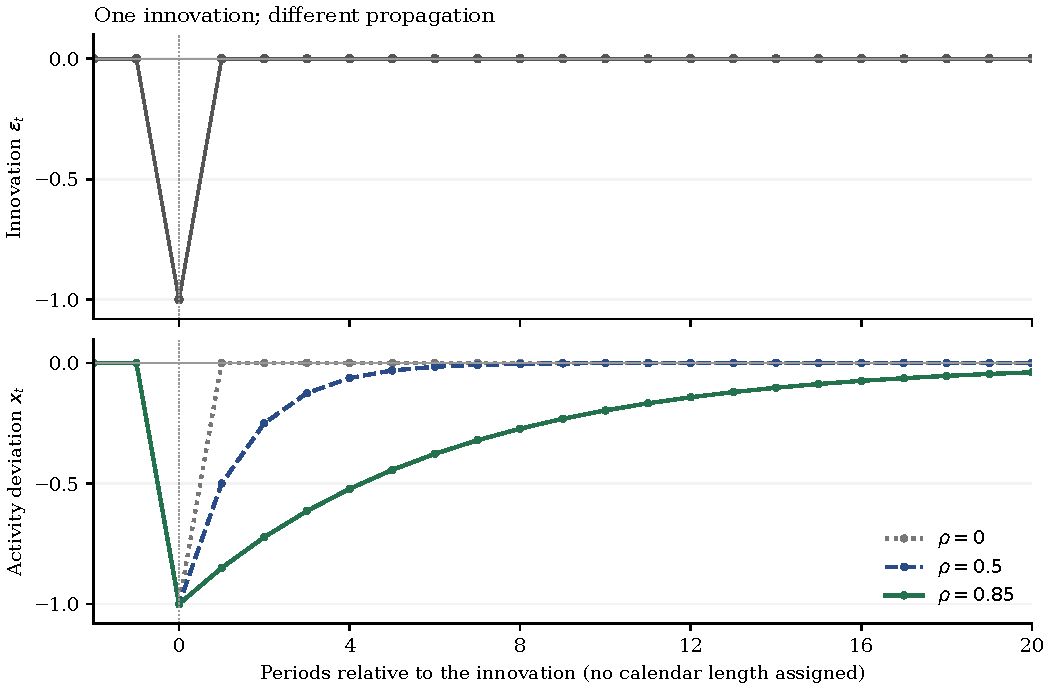
\includegraphics[width=\linewidth]{fluctuation_impulse_propagation.pdf}
\caption{The same one-period negative innovation with different assumed
persistence coefficients. All paths have the same impact. The lower panel
shows subsequent activity, not additional shocks. Periods have no assigned
calendar length, and the curves are not estimates.}
\label{fig:fluctuation-propagation}
\end{figure}

The accumulated deviation in this stable example is
$\sum_{t=0}^{\infty}x_t=-1/(1-\rho)$. That is an area in units of the
chosen deviation, not a welfare measure or an identified amount of GDP lost.
It shows why impact size alone is insufficient to describe a disturbance.
Figure~\ref{fig:fluctuation-propagation} holds the impact fixed to isolate
persistence; a full model can change impact and duration together.

\subsubsection{Individual plans meet through income, prices, and constraints}

A household can try to improve its finances by spending less. If many
households do so together, their suppliers' revenues change. It is then
necessary to explain how saving reaches investment, how prices and interest
rates respond, and whether output or employment adjusts. Planned saving
is not an extra stock of goods available independently of those responses.

In a flexible-price economy with effective intermediation, some adjustment
may occur through relative prices and intertemporal substitution. With
sticky prices, pessimistic expected sales, or binding financing constraints,
the same initial spending intention can produce a different output response.
The paradox of thrift is a conditional general-equilibrium mechanism, not
a statement that saving is always harmful. It is consistent with the growth
chapters' finding that accumulation can improve future opportunities.

The same principle applies to a firm cutting wages or costs: an individually
sensible response changes other people's income and choices. Individual
optimization does not by itself guarantee an efficient aggregate outcome
when externalities or other distortions are present. Conversely, adjustment
to a genuinely reduced production opportunity can lower output even in an
efficient equilibrium. Falling output alone does not choose between these
accounts.

\subsection{Do fluctuations belong to the short, medium, or long run?}

\subsubsection{The relevant clock is the adjustment mechanism}

Business-cycle analysis often focuses on changes over quarters and years.
That is a useful scale for production, spending, and employment decisions;
it is not a definition that all effects expire within a fixed number of years.
Short, medium, and long run describe which adjustments have had time to
occur. Those adjustments overlap rather than occupying sealed calendar boxes.

\Needspace{23\baselineskip}
\begin{center}
\small
\begin{tabular}{p{0.18\linewidth}p{0.34\linewidth}p{0.34\linewidth}}
\hline
\tableheading{Perspective} & \tableheading{Adjustments to examine} & \tableheading{Why an effect may remain}\\
\hline
Short run & Orders, inventories, hours, spending, prices, and contracts &
Existing commitments or constraints can prevent immediate reallocation\\[4pt]
Medium run & Hiring, matching, capital installation, sectoral movement, and debt repair &
Stocks, skills, and financial positions take time to rebuild or reorganize\\[4pt]
Long run & Productive capacity, institutions, research, and paths of technology and population &
Earlier decisions can alter the stocks or accumulation mechanisms that support later activity\\
\hline
\end{tabular}
\end{center}

A price can change quickly while a borrower remains heavily indebted.
Construction can stop immediately although an unfinished plant takes years
to repurpose. Employment can recover in aggregate while displaced workers
still need different skills. The appropriate horizon depends on the question
and the constraints that remain, not simply on how much time has passed.

Financial movements can also have a different timescale from measured
business-cycle movements. Drehmann, Borio, and Tsatsaronis (2012) document
longer movements in credit and property prices in their historical financial-
cycle analysis.\footnote{Mathias Drehmann, Claudio Borio, and Kostas
Tsatsaronis (2012), ``Characterising the Financial Cycle: Don't Lose Sight
of the Medium Term!'' \textit{BIS Working Papers}, no.~380.
\url{https://www.bis.org/publ/work380.htm}. This is evidence under that
paper's definition and sample, not a universal period for every credit cycle.}
A short recovery in spending need not complete balance-sheet repair. Nor
does a longer financial movement establish that every business cycle began
in finance.

\subsubsection{Shock duration, recovery time, and lasting damage are different}

A shipping interruption might end quickly while inventories, production
schedules, and customers' orders take longer to normalize. A persistent
rise in energy costs may require a new production mix instead of restoration
of the old one. A brief period without credit might close a firm whose
customer relationships cannot be recreated immediately.

The growth chapters make these links explicit. Less investment changes
future capital. Less training can change skills. Research cuts or reduced
entry can change later innovation. Not every temporary reduction produces
a permanent effect: replacement investment, rehiring, catch-up, or new entry
can restore the previous path under suitable conditions. The adjustment
mechanism must determine whether and how that happens.

In the strict sense, hysteresis means that history changes the economy's
long-run outcome, rather than merely producing slow convergence to the same
one. Blanchard and Summers' analysis of European unemployment is a classic
application of this idea.\footnote{Olivier J. Blanchard and Lawrence H.
Summers (1986), ``Hysteresis and the European Unemployment Problem,''
\textit{NBER Macroeconomics Annual}, 1, 15--78; working-paper version:
\url{https://www.nber.org/papers/w1950}.}
The term should not substitute for a mechanism. Lost skills, disrupted job
matching, and a temporary hiring delay have different implications for
whether an effect eventually disappears.

Cerra and Saxena (2008) provide historical cross-country evidence of highly
persistent output losses after financial crises and some political crises.
\footnote{Valerie Cerra and Sweta Chaman Saxena (2008), ``Growth Dynamics:
The Myth of Economic Recovery,'' \textit{American Economic Review}, 98(1),
439--457. \url{https://doi.org/10.1257/aer.98.1.439}. The statement concerns
the crises and methods studied there, not an inevitability for every downturn.}
This is a reason to investigate lasting losses, not permission to label every
estimated trend break as the causal effect of a recession. The earlier
forecast may have been too optimistic, and the disturbance may itself have
changed productive opportunities.

\Needspace{11\baselineskip}
\begin{blueblock}
\textbf{Long-run adjustment does not mean returning to the old forecast.}
A model can have flexible prices in the long run and still inherit different
capital, skills, debt, or technology after a downturn. A permanent level loss,
a permanently lower growth rate, and slow recovery to an unchanged path are
different outcomes. The time horizon alone does not tell us which one occurs.
\end{blueblock}

\subsection{Why do fluctuations matter?}

\subsubsection{Lost activity and displaced people are not just a line on a graph}

An unsold service today may never be produced later. A later increase in
output need not replace the consumption or work experience that was missed.
Returning to an earlier output level also falls short of a counterfactual
path that would have continued growing. The benchmark must still be justified
before a cumulative shortfall is interpreted as avoidable lost production.

Households experience the same aggregate movement differently. A worker
losing a job, a borrower facing refinancing, a retiree with fixed nominal
claims, and a firm with cash reserves face different risks. Aggregate
consumption can appear stable while losses concentrate among people who
cannot insure them. Inflation and asset-price changes can redistribute
purchasing power as well as change aggregate activity.

The costs include consumption risk, involuntary loss of work, disruption
of productive relationships, and possible changes in future opportunities.
An expansion can also involve excessive risk-taking or distorted allocation
under particular incentives. The welfare object is therefore richer than
minimizing the variance of GDP around a fitted trend.

\subsubsection{Even fluctuations around the same mean can be costly}

A small example isolates consumption risk. Suppose a person has log utility
and faces two equally likely consumption outcomes, $0.9$ and $1.1$, with
no way to insure or transfer resources between them. Expected consumption
is one, but expected utility is
\[
\tfrac12\log(0.9)+\tfrac12\log(1.1)
=\tfrac12\log(0.99)<\log(1)=0.
\]
The certain consumption giving the same utility is
$\sqrt{0.99}\simeq0.99499$. Eliminating this particular risk at unchanged
mean consumption would be desirable to this person. It does not tell us the
aggregate welfare cost of business cycles: insurance, leisure, heterogeneity,
expected growth, and the cost of changing the fluctuations are absent.

The example illustrates a reason to care about risk. It does not imply
that every observed output movement should be prevented. If an input becomes
scarce, an efficient economy may produce less and alter its consumption mix.
If a price or credit distortion causes additional unemployment and lost
trade, reducing that distortion poses a different welfare problem.

\Needspace{11\baselineskip}
\begin{redblock}
\textbf{Question: the same fall in output, three different economies.}
In one economy, a missing input makes production infeasible. In another,
customers postpone purchases while goods prices adjust slowly. In a third,
firms have orders but lose access to working funds. Ask what limits production
in each, what happens to prices and employment, and which intervention changes
the relevant constraint. The observed fall in GDP is insufficient to prescribe
the same response in all three.
\end{redblock}

Policy can cushion income risk, support spending, repair intermediation,
or help resources adjust. Each intervention has a channel, financing,
incentive effects, and implementation limits. Supporting demand does not
manufacture a missing component; increasing productive capacity does not
ensure it will be purchased now. Some episodes require several responses
because the initial disturbance creates new constraints as it propagates.

\subsection{What must a model of fluctuations explain?}

A convincing account should explain a joint path: production and spending,
employment and hours, prices and wages, investment and finance. It should
say what initiated the change, what was already anticipated, why other
agents responded, and why the response took the observed time to unfold.
Matching the movement of GDP alone can leave very different explanations
observationally similar.

A useful empirical distinction is between an unconditional regularity and
a response to a specified shock. Output and employment moving together
in the data does not establish how either responds to a technology shock,
for example: the data contain several disturbances and policy responses.
An impulse response asks what follows a particular innovation relative
to a specified comparison path. Its interpretation depends on how that
innovation was identified.

The next chapter starts with RBC because it carries the Ramsey logic
into changing real opportunities and endogenous labor choices. It gives a
benchmark for asking how much individual adjustment and inherited capital
can explain under flexible prices. The order of presentation does not
establish that technology causes all fluctuations, that money is irrelevant,
or that all unemployment is an efficient choice. Those are claims requiring
specific assumptions and evidence.

New Keynesian and sticky-wage models then make nominal adjustment part of
the explanation. Labor-market models examine hiring and matching, while
later chapters develop financial and distributional transmission. The models
will earn their place by explaining a mechanism and its limits. Keep the
factory's questions in view: what changed first, what carried the change,
who bore it, and which opportunities remained different afterward?

% !TEX root = ../macro.tex
\section{Real Business Cycle Model}\label{sec:rbc}

% BEGIN ORIGINAL RBC COURSE TEXT (pre-revision; comparison only)
% 
% Originated from Kyland and Prescott (1982), Long and Plosser (1983), RBC model shows great empirical importance. A standard RBC model\footnote{For a sound review over the topic of RBC, see Rebelo Sergio. 2005. “Real Business Cycle Models: Past, Present, and Future.” The Scandinavian Journal of Economics. } is in nature a Ramsey model with
% \begin{itemize}
% \tightlist
%   \item Endogenous (but constant in the long run, i.e. $n = 0$) labor supply
%   \item Stochastic productivity (i.e. real shocks)
% \end{itemize}
% 
% 
% \begin{blueblock}
% \begin{note}[Two principles of the RBC theory of business cycles]
% 
% 1. Money is of little importance in business cycles.
% 
% 2. Business cycles are created by rational agents responding optimally to
% real (not nominal) shocks - mostly fluctuations in productivity growth,
% but also fluctuations in government purchases, import prices, or preferences.
% \end{note}
% \end{blueblock}
% 
% 
% 
% 
% \sepline
% \subsection{UMP of household}
% A typical household entails product-consuming for $C_t$ and labor-providing for $N_t$. Only in this model, the agent value leisure $L_t=1-N_t$.
% 
% The UMP in RBC model is
% \begin{align}
% &\max\limits_{C_{t},N_{t},B_{t}} E_t \sum\limits_{t=0}^{\infty}\beta^{t}u(C_{t},N_{t})
% \\&
% s.t. \; P_{t}C_{t}+Q_{t}B_{t}\leqslant B_{t-1}+W_{t}N_{t}+D_{t}
% \text{, where }
% \begin{cases}
% \beta \in (0,1) \\
% Q_{t}=\frac{1}{1+i_{t}} \text{ is the price per bond bought today}
% \end{cases}
% \end{align}
% 
% Form a Lagrangian and acquire FOCs
% \begin{align}
% &\mathscr{L}=E_{0} \sum\limits_{t=0}^{\infty}\beta^{t}[u(C_{t},N_{t})+\lambda_{t}(P_{t}C_{t}+Q_{t}B_{t}-B_{t-1}-W_{t}N_{t}-D_{t} )]
% \\&
% \Rightarrow
% \begin{cases}\frac{\partial  \mathscr{L}}{\partial C_{t}}=0 \Rightarrow \beta^{t}[u_{C_{t}} -\lambda_{t}P_{t}]=0 \Rightarrow \frac{u_{C_{t}}}{E_{t}U_{c,t+1}}=\frac{\lambda_{t}}{E_{t}\lambda_{t+1}} \cdot \frac{P_{t}}{E_{t}{P_{t+1}}} \\
% \frac{\partial  \mathscr{L}}{\partial N_{t}}=0 \Rightarrow \beta^{t}[u_{N_{t}}+\lambda_{t} W_{t}] =0 \\
% \frac{\partial  \mathscr{L}}{\partial B_{t}}=0 \Rightarrow -\lambda_{t}Q_{t}\beta^{t}+E_{t}\lambda_{t+1}\beta^{t+1}=0 \Rightarrow \beta \frac{E_{t}\lambda_{t+1}}{\lambda_{t}}=Q_{t} \Rightarrow \frac{1}{Q_{t}}=1+i_{t}
% \end{cases}
% \end{align}
% 
% using these FOCs
% \begin{align}
% &\begin{cases}
%   \beta^{t}[u_{C_{t}} -\lambda_{t}P_{t}]=0 \\
%   \beta^{t}[u_{N_{t}}+\lambda_{t} W_{t}] =0
% \end{cases} \Rightarrow \color{red} \text{Labor supply equation} -\frac{u_{N_{t}}}{u_{C_{t}}}=\frac{W_{t}}{P_{t}}
% \\&
% \text{Also} \begin{cases}\frac{u_{C_{t}}}{E_{t}U_{c,t+1}}=\frac{\lambda_{t}}{E_{t}\lambda_{t+1}} \cdot \frac{P_{t}}{E_{t}{P_{t+1}}} \\
% \beta \frac{E_{t}\lambda_{t+1}}{\lambda_{t}}=Q_{t}
% \end{cases}
% \Rightarrow \color{red} \text{Euler's equation } \frac{Q_{t}}{\beta}=E_{t}\cdot
% \frac{\frac{U_{c,t+1}}{P_{t+1}}}{\frac{U_{c,t}}{P_{t}}}
% \end{align}
% 
% 
% \begin{greenblock}
% e.g. Let utility function be specific
% \begin{align}
% &
% u(C_{t},N_{t})=\begin{cases}
% \frac{c^{1-\sigma}_{t}-1}{1-\sigma}-\frac{N_{t}^{1+\varphi}}{1+\varphi},\sigma\neq 1 \\
% \log C_{t}-\frac{N_{t}^{1+\varphi}}{1+\varphi},\sigma=1\end{cases}
% \\&
% \Rightarrow \begin{cases}
% \frac{W_{t}}{P_{t}}=C_{t}^{\sigma}N_{t}^{\varphi} \\
% Q_{t}=\beta E_{t}\cdot (\frac{C_{t+1}}{C_{t}})^{-\sigma}\cdot \frac{P_{t}}{P_{t+1}}
% \end{cases}
% \end{align}
% \end{greenblock}
% 
% 
% 
% \sepline
% \subsection{PMP of firm}
% \begin{align}
% \min\limits_{N_{t}} W_t N_t \Leftrightarrow &\max\limits_{Y_t} P_{t}Y_{t}-W_{t}N_{t}
% \\&s.t. Y_t = A_t K_t^\alpha N_t^{1-\alpha}, \alpha \in [0,1)
% \\&
% \text{where }
% \begin{cases}
%   Y_{t}=A_{t}W_{t}^{1-\alpha}\\
%   A_{t}=A_{t-1}^{\rho\alpha} \epsilon_{t}^{\alpha}, \epsilon_{t}^{\alpha} \overset{iid}{\sim} N(0,\sigma_{\alpha}^{\epsilon})
%   \text{ (technology shocks)}
% \end{cases}
% \\&
% \Rightarrow \text{F.O.C.: } \frac{W_{t}}{P_{t}}=(1-\alpha)A_{t}N_{t}^{-\alpha} \text{ (labor demand equation)}
% \end{align}
% 
% \sepline
% \subsection{Economy described by RBC}
% {\color{red}
% The whole economy system is described as the balance of demand and supply
% \begin{align}
% &\text{AS}
% \begin{cases} Y_{t}=A_{t}N_{t}^{1-\alpha} \text{ (total production function)}, A_t=A^{\rho a}_{t-1} e^{\epsilon^a_t} \text{ (technology shocks)}\\
% \frac{W_{t}}{P_{t}}=C_{t}^{\sigma}N_{t}^{\varphi} \text{ (labor supply from UMP)}\\
% \frac{w_{t}}{P_{t}}=(1-\alpha)A_{t}N_{t}^{-\alpha} \text{ (labor demand from PMP)}
% \end{cases}
% \\&
% \text{AD}
% \begin{cases}Y_{t}=C_{t}+I_{t} \text{ (accouting equation)}\\
% Q_{t}=\beta E_{t} (\frac{C_{t+1}}{C_{t}})^{-a} \frac{P_{t}}{P_{t+1}}  \text{ (Euler equation from UMP)}\\
% \frac{M_{t}}{P_{t}}=\frac{Y_{t}}{Q_{t}^{-n}}  \text{ (demand of liquidity)}
% \end{cases}
% \end{align}
% }
% 
% 
% \sepline
% \subsection{Log-linearization}
% 
% Two methods we can transform.
% 1) The first is
% \begin{align}
% &
% \hat x_{t}=\ln x_{t}-\ln x^{*}
% \\&
% =\ln |\frac{ x_{t}}{x^{*}}|
% \\&
% =\ln |1+ \frac{x_{t}-x^{*}}{x^{*}}| \text{ (percentage of deviation from stable state)}
% \\&
% \approx \ln |1+\frac{1}{x^{*}}(x_{t}-x^{*})|
% \\&
% =\frac{x_{t}-x^{*}}{x^{*}}
% \end{align}
% 
% 2) Another approach would be
% \begin{align}
% &\ln x^{*}=ln x_{t}-\tilde{x_{t}}\Rightarrow \ln x_{t}=ln x^{*}+\tilde{x_{t}}
% \\&
% \Rightarrow e^{\ln x_{t}}=x_{t}=e^{n x^{*}+\tilde{x_{t}}}=x^{*}e^{\hat{x_{t}}} \approx x^{*} (1+\hat x_{t})
% \end{align}
% 
% Now we turn to the linearization of RBC model
% \begin{align}
% &
% \begin{cases}
% y_{t}=a_{t}+(1-\alpha)n_{t}
% \\
% y=a+(1-\alpha)n
% \end{cases}
% \Rightarrow \hat y_{t}=\hat a_{t}+(1-\alpha)\hat n_{t}
% \\&
% \Rightarrow
% \begin{cases}
% \hat w_{t}-\hat p_{t}=\hat a_{t}+(1-\alpha)\hat n_{t} \\
% \hat w_{t}-\hat p_{t}=a\hat c_{t}+\rho \hat n_{t}\end{cases}
% \Rightarrow \hat y_{t}=\hat c_{t}, \; m_{t}-\hat p_{t}=\hat y_{t} -\hat n_{it}
% \\&
% Y_{t}=C_{t}+I_{t}
% \\&
% Y\cdot e^{\hat y_{t}}=C\cdot e^{\hat c_{t}}+I\cdot e^{\hat i_{t}}
% \\&
% Y(1+\hat y_{t})=C(1+\hat c_{t})+I(1+\hat i_{t})
% \\&
% \hat y_{t}=\frac{C}{Y}\hat c_{t}+ \frac{I}{Y} \hat i_{t}\\&
% a_{t}=\rho_{t} a_{t-1}+\epsilon_{t}^{a}
% \\&
% 1=E_{t} e^{\ln \beta + +\ln \frac{1}{Q_{t}}-a(c_{t+1}-c_{t})-(P_{t+1}-P_{t})}
% \\&
% 1=E_{t} e^{\ln \beta + +\ln \frac{1}{Q_{t}}-a\triangle c_{t+1}-\pi_{t+1}}
% \\&
% 1=E_{t} I[1+(i_{t}-i)-a(\triangle c_{t+1}-\triangle c_{t}]-(\pi_{t+1}-\pi_{t})]
% \end{align}
% 
% {\color{red} Therefore a RBC model can be rewritten in linearized log equations
% \begin{align}
% \color{red}&\text{AS:} \begin{cases}
% \hat y_{t}=a_{t}+(1-\alpha)\hat n_{t} \text{ (output)}\\
% \hat w_{t}-\hat p_{t}=a_{t}-\alpha \hat n_{t} \text{ (labor demand)}\\
% \hat w_{t}-\hat p_{t}=a c_{t}+\varphi \hat n_{t} \text{ (labor supply)}\\
% \hat a_{t}=\rho_a \hat a_{t-1}+\epsilon_t^a \text{ (technology)}
% \end{cases}
% \\&
% \text{AD:} \begin{cases}
% \hat y_{t}=\hat c_{t} \text{ (product market clearing)}\\
% \hat c_{t}=E_{t}\hat c_{t+1}-\frac{1}{a}(\hat i_{t}-E_{t}\hat \pi_{t+1}) \\
% \hat m_{t}-\hat p_{t}=\hat y_{t}-\eta \cdot \hat i_{t} \text{ (money demand equation; $\eta$ is interest rate elasticity)}\\
% \hat r_{t}=i_{t}-E_{t} \hat \pi_{t+1} \text{ (Fisherian equation)}
% \end{cases}
% \end{align}
% }
% 
% \begin{blueblock}
% \begin{note}[Exceptation for Expectation]
% Notice this method does not apply to equations involving expectations.
% \end{note}
% \end{blueblock}
% 
% \begin{blueblock}
% \begin{note}[RBC has neutrality of money]
% The final answer of this standard RBC model is not relevant to any price variable, inferring the model being money-neutral.
% \end{note}
% \end{blueblock}
% 
% 
% 
% 
% 
% 
% 
% 
% 
% \subsection[Capital accumulation and investment (planned)]{Capital accumulation and investment}
% \textit{Planned section.} Extend the current fixed-capital benchmark to endogenous capital accumulation.
% Derive investment dynamics and distinguish the simplified benchmark from a
% full RBC model with a changing capital stock.
% END ORIGINAL RBC COURSE TEXT

\subsection{From a growth path to changing opportunities}

\subsubsection{What would make a Ramsey household change its working week?}

Imagine a group of factories. Their machines have not changed overnight, but
an interruption in power supply now makes each working shift less productive.
Orders, hours, investment, and consumption may all change. Start with questions
rather than labeling the event a ``technology shock.'' Can the factories produce
less with the same inputs? Are households poorer? Should they postpone work or
investment until conditions improve? Would the answer differ if the interruption
lasted one week rather than several years?

Ramsey already gives a way to compare consumption today and tomorrow. But with
fixed labor and a known production path, it leaves two margins closed. Households
cannot move working time toward more rewarding dates, and they never have to
choose before learning tomorrow's production conditions. Let labor be chosen;
let future productivity be uncertain. Keep preferences, ownership, production,
and market clearing explicit. This produces a tractable real business cycle
(RBC) benchmark.

This is a teaching reconstruction of the modeling questions, not a record of
any author's private thought process. Kydland and Prescott (1982) and Long and
Plosser (1983) are foundational contributions. Their actual environments differ;
the one-sector model below is a simpler teaching economy, without the former's
multi-period construction technology or the latter's sectoral structure.
\footnote{Finn E. Kydland and Edward C. Prescott (1982), ``Time to Build and
Aggregate Fluctuations,'' \textit{Econometrica}, 50(6), 1345--1370,
\url{https://www.minneapolisfed.org/~/media/files/research/prescott/papers/timetobuild.pdf};
John B. Long, Jr., and Charles I. Plosser (1983), ``Real Business Cycles,''
\textit{Journal of Political Economy}, 91(1), 39--69,
\url{https://doi.org/10.1086/261128}.}

\subsubsection{Choose the disturbance, then explain its transmission}

A scalar $A_t$ summarizes how much output given capital and hours can produce.
An unexpected change in it is an innovation. The persistence of $A_t$ describes
how long production opportunities change. Household choices and accumulated
capital determine how that change travels through the economy. These are three
different objects: innovation, persistence, and propagation.

A fall in $A_t$ need not mean that engineers forgot a blueprint. A power or
logistics disruption can reduce effective production opportunities. But treating
an event as a scalar productivity change is a modeling decision: energy inputs,
relative prices, network bottlenecks, and distributional losses have been
suppressed. A credit refusal or an absence of orders cannot automatically be
reclassified as technology. Their mechanisms need their own constraints.

The growth models explain accumulation and, in some cases, the source of trend
growth. Here we hold trend productivity constant to isolate fluctuations around
a stationary reference. This does not assert that actual output has no trend.
Adding a deterministic trend requires a consistent normalization of production,
preferences, and Euler conditions; it cannot be hidden inside the shock term.

\Needspace{11\baselineskip}
\begin{blueblock}
\textbf{A real benchmark is a conditional experiment.}
The original course principles become two questions. How much joint movement
can real disturbances produce when agents respond optimally? Which observed
movements require additional mechanisms? Money and nominal frictions are
excluded from the real allocation block below. Their exclusion does not
establish their empirical irrelevance. Government purchases, relative import
prices, and preference disturbances can be studied in extensions, but are not
silently included in this one-shock economy.
\end{blueblock}

\subsection{Complete conditions and the order of decisions}\label{sec:rbc-conditions}

The main model has endogenous capital. The course's fixed-capital benchmark
will be recovered as a separate restriction in Section~\ref{sec:rbc-fixed}.
Population is one and does not grow; hours are allowed to vary at every date.
In particular, zero population growth is not constant labor input.

\Needspace{18\baselineskip}
\begin{modelsetup}[1]
\begin{modelcondition}{01}{Dates, people, and the time endowment}
Time is discrete, $t=0,1,\ldots$. A closed economy contains many identical,
infinite-lived, price-taking households, aggregated to one representative
household of constant mass one. Each household has one unit of time per date:
$N_t\in[0,1]$ is work and $L_t=1-N_t$ is leisure. Work denotes an intensive
hours margin; there is no separate unemployment, participation, matching, or
involuntary rationing margin. Consumption satisfies $C_t>0$.
\end{modelcondition}
\begin{modelcondition}{02}{Goods, states, ownership, and timing}
One homogeneous good can be consumed or installed as capital at unit resource
cost. Households own the capital and firm shares. The given initial stock is
$K_0>0$; $K_t$ was chosen at $t-1$ and is usable at $t$. The current productivity
$A_t$ is observed before choosing $C_t,N_t,I_t,K_{t+1}$ and financial positions.
Next period's innovation is not yet observed. Capital is the only accumulated
productive stock; there are no inventories, skills, adjustment costs,
installation delays, or variable utilization in this benchmark.
\end{modelcondition}
\begin{modelcondition}{03}{Production and competitive firms}
Firms rent capital and hire labor in competitive spot markets. Their technology
is $Y_t=A_tK_t^\alpha N_t^{1-\alpha}$, with $A_t>0$ and $0<\alpha<1$.
It has constant returns in $(K_t,N_t)$, positive marginal products, and diminishing
marginal products holding the other input fixed. Firms take prices and $A_t$
as given; there is no markup, externality, or nominal price or wage rigidity.
\end{modelcondition}
\begin{modelcondition}{04}{The stochastic process and information}
Write $a_t=\log(A_t/\bar A)$, where $\bar A>0$, and let
\[
a_t=\rho_a a_{t-1}+\varepsilon_t^a,\qquad |\rho_a|<1,\qquad
E_{t-1}\varepsilon_t^a=0,\quad E[(\varepsilon_t^a)^2]=s_\varepsilon^2<\infty.
\]
Innovations are independent and identically distributed, with a distribution
known to households; Gaussian innovations are an optional specification.
$E_t$ conditions on the full observed history through $t$ and the equilibrium
rules, including current $K_t,A_t$. Rational expectations means using this
conditional law, not knowing the future realization. $a_t=0$ is the deterministic
reference, not a claim that $E A_t=\bar A$ under uncertainty.
\end{modelcondition}
\begin{modelcondition}{05}{Preferences and the household objective}
The household maximizes $E_0\sum_{t=0}^\infty\beta^t u(C_t,N_t)$, with
$0<\beta<1$, $\sigma>0$, $\chi>0$, and $\varphi>0$, where
\[
u(C,N)=
\begin{cases}
(C^{1-\sigma}-1)/(1-\sigma)-\chi N^{1+\varphi}/(1+\varphi),&\sigma\ne1,\\
\log C-\chi N^{1+\varphi}/(1+\varphi),&\sigma=1.
\end{cases}
\]
The original course normalization is $\chi=1$. $\sigma$ governs consumption
curvature; $\varphi$ governs the curvature of work disutility. We derive local
interior conditions with $0<N_t<1$. Parameter and shock choices must support
finite expected welfare and feasible paths; large shocks may activate corners
that a local solution does not describe.
\end{modelcondition}
\begin{modelcondition}{06}{Accumulation, prices, and household resources}
Capital depreciates at $0<\delta<1$ and satisfies
$K_{t+1}=(1-\delta)K_t+I_t\geq0$. The baseline permits reversible investment;
there is no additional $I_t\geq0$ constraint. Let $w_t$ be the real wage,
$q_t$ the real capital rental payment before depreciation, and $d_t$ real
profits distributed to households. With no financial trade the household budget is
\[
C_t+K_{t+1}=w_tN_t+(q_t+1-\delta)K_t+d_t.
\]
Households face no tax, transfer, borrowing wedge, or idiosyncratic uninsured
risk. Prices and returns are taken as given in individual optimization;
market clearing is imposed afterward.
\end{modelcondition}
\begin{modelcondition}{07}{Financial claims and nominal units}
For the course's nominal bond calculation, $P_t>0$ is the goods price,
$W_t=P_tw_t$, and $D_t=P_td_t$. $B_t$ pays one currency unit per unit at $t+1$
and costs $Q_t>0$ at $t$, so $R_t^n=1/Q_t=1+i_t$ is the gross nominal return.
The full budget is
\[
P_t[C_t+K_{t+1}-(1-\delta)K_t]+Q_tB_t
 =W_tN_t+P_tq_tK_t+B_{t-1}+D_t.
\]
Bonds are in zero aggregate net supply and $B_{-1}=0$. A household's small
financial trade is allowed when deriving its Euler condition; identical-agent
market clearing then sets aggregate $B_t=0$. A risk-free \emph{real} claim is
a separate hypothetical payoff, not the nominal bond deflated by a known
future price. There is no monetary asset in the core household budget.
\end{modelcondition}
\begin{modelcondition}{08}{Market clearing, solvency, and terminal behavior}
Household labor and capital supplies equal firms' demands. Goods clear as
$Y_t=C_t+I_t$, and constant returns with competitive pricing imply $d_t=0$.
Admissible household plans rule out debt rollovers that finance consumption
without resources. For the capital-only aggregate optimum the transversality
restriction is
\[
\lim_{T\to\infty}E_0[\beta^T C_T^{-\sigma}K_{T+1}]=0.
\]
Solvency restricts admissible borrowing; transversality selects optimal terminal
behavior. Neither follows merely from writing the interior Euler equations.
No-Ponzi restrictions also apply to any individual financial trades.
\end{modelcondition}
\begin{modelcondition}{09}{Equilibrium, reference state, and scope}
An equilibrium is a collection of history-contingent allocations and prices
satisfying household optimality and admissibility, firm optimality, the
productivity law, and all market-clearing conditions for the given initial
state. We select the locally stable interior solution near its deterministic
steady state. Money, government, foreign trade, monopoly, financial frictions,
and household heterogeneity are absent. A nominal policy or quantity closure
is an extra specification; the real equations alone do not select $P_t$.
\end{modelcondition}
\end{modelsetup}

The within-date sequence is
\[
\underbrace{K_t,\ A_t\text{ observed}}_{\text{inherited stock and current information}}
\ \longrightarrow\
\underbrace{N_t,\ Y_t,\ C_t,\ I_t}_{\text{work, production, and allocation}}
\ \longrightarrow\
\underbrace{K_{t+1}}_{\text{productive next date}}.
\]
An announcement about tomorrow can change today's choices; tomorrow's machine
stock cannot jump retroactively. In the experiment below only unanticipated
productivity innovations occur.

\subsection{Household choice: working now and transferring consumption}

\subsubsection{Retain the course's nominal bond route}

First suppress capital trade to isolate the original asset calculation. Write
nominal nonlabor income as $\mathcal D_t$; this includes the fixed factor's
income in the course benchmark. The budget is
\begin{equation}\label{eq:rbc-course-budget}
P_tC_t+Q_tB_t=B_{t-1}+W_tN_t+\mathcal D_t.
\end{equation}
Use resources minus expenditures in the multiplier term:
\begin{equation}
\mathscr L=E_0\sum_{t=0}^\infty\beta^t
\{u(C_t,N_t)+\lambda_t[B_{t-1}+W_tN_t+\mathcal D_t-P_tC_t-Q_tB_t]\}.
\end{equation}
For an interior choice at a history observed at $t$, the first two derivatives are
\begin{align}
u_{C,t}-\lambda_tP_t&=0,
 &\lambda_t&=u_{C,t}/P_t,\\
u_{N,t}+\lambda_tW_t&=0,
 &-u_{N,t}&=\lambda_tW_t.
\end{align}
The common factor $\beta^t$ and the probability of reaching this history cancel
from the two conditions. Divide the second condition by the first:
\begin{align}
\frac{-u_{N,t}}{u_{C,t}}&=\frac{\lambda_tW_t}{\lambda_tP_t},\\
-\frac{u_{N,t}}{u_{C,t}}&=\frac{W_t}{P_t}=w_t.\label{eq:rbc-labor-general}
\end{align}
The marginal disutility of another working hour equals its consumption-valued
wage. This is an intratemporal condition: all its objects are known at $t$.

One unit of $B_t$ costs $Q_t$ now and pays one currency unit in every next-date
state. Its two multiplier contributions give
\begin{align}
0&=-\beta^t\lambda_tQ_t+\beta^{t+1}E_t\lambda_{t+1},\\
\lambda_tQ_t&=\beta E_t\lambda_{t+1},\\
Q_t\frac{u_{C,t}}{P_t}&=\beta E_t\!\left[\frac{u_{C,t+1}}{P_{t+1}}\right],\\
Q_t&=\beta E_t\!\left[
\frac{u_{C,t+1}}{u_{C,t}}\frac{P_t}{P_{t+1}}\right].\label{eq:rbc-nominal-euler}
\end{align}
Current $P_t$ and $u_{C,t}$ can leave the expectation; future marginal utility
and the future price generally cannot. The last line retains the course's
nominal Euler equation with a consistent sign and information convention.

Differentiate the stated utility explicitly:
\begin{align}
\frac{d}{dC}\frac{C^{1-\sigma}-1}{1-\sigma}
 &=\frac{(1-\sigma)C^{-\sigma}}{1-\sigma}=C^{-\sigma},\\
\frac{d}{dC}\log C&=1/C=C^{-1},\\
\frac{\partial u}{\partial N}
 &=-\frac{\chi(1+\varphi)N^\varphi}{1+\varphi}=-\chi N^\varphi.
\end{align}
Substitution into the two optimality conditions yields
\begin{align}
-\frac{-\chi N_t^\varphi}{C_t^{-\sigma}}
 &=\chi C_t^\sigma N_t^\varphi=w_t,\label{eq:rbc-labor}\\
\frac{u_{C,t+1}}{u_{C,t}}
 &=\frac{C_{t+1}^{-\sigma}}{C_t^{-\sigma}}
   =\left(\frac{C_{t+1}}{C_t}\right)^{-\sigma},\\
Q_t&=\beta E_t\!\left[
\left(\frac{C_{t+1}}{C_t}\right)^{-\sigma}
\frac{P_t}{P_{t+1}}\right].\label{eq:rbc-bond-crra}
\end{align}
When $C_t$ and thus the marginal value of resources are held fixed,
\begin{align}
\log N_t&=\frac{\log w_t-\log\chi-\sigma\log C_t}{\varphi},\\
\left.\frac{\partial\log N_t}{\partial\log w_t}\right|_{u_{C,t}}
 &=1/\varphi.
\end{align}
This is the Frisch hours elasticity. Along an equilibrium, consumption also
changes: a higher wage creates both a reward to working and additional wealth.
The Frisch calculation alone does not determine the total hours response.

\Needspace{12\baselineskip}
\begin{blueblock}
\textbf{Keep random prices inside the expectation.}
In general $E_t(X/Z)\ne E_tX/E_tZ$, and $E_t(XZ)\ne E_tX\,E_tZ$.
For two equally likely future states with $(X,Z)=(1,1),(3,2)$,
\[
E(X/Z)=\tfrac12(1+3/2)=5/4,\qquad EX/EZ=2/(3/2)=4/3.
\]
The nominal bond pays a certain currency amount, but its purchasing power
$1/P_{t+1}$ is uncertain. A risk-free real bond instead has a certain goods
payoff. Confusing the two loses the connection between prices and consumption
risk.
\end{blueblock}

\subsubsection{Capital brings back the Ramsey margin, with uncertain returns}

For the full budget in card 07, consumption and hours have the same derivatives.
The cost of one extra unit of $K_{t+1}$ is $P_t$ at $t$. Next date it delivers
rental income $P_{t+1}q_{t+1}$ plus surviving capital $P_{t+1}(1-\delta)$.
Taking prices as given, the two-date derivative is
\begin{align}
0&=-\beta^t\lambda_tP_t
 +\beta^{t+1}E_t[\lambda_{t+1}P_{t+1}(q_{t+1}+1-\delta)],\\
\lambda_tP_t
 &=\beta E_t[\lambda_{t+1}P_{t+1}(q_{t+1}+1-\delta)],\\
C_t^{-\sigma}
 &=\beta E_t[C_{t+1}^{-\sigma}(q_{t+1}+1-\delta)].\label{eq:rbc-capital-euler}
\end{align}
Let $R^K_{t+1}=q_{t+1}+1-\delta$ and
$M_{t,t+1}=\beta(C_{t+1}/C_t)^{-\sigma}$. Division by current marginal utility gives
\begin{align}
1&=E_t[M_{t,t+1}R^K_{t+1}],\\
Q_t&=E_t[M_{t,t+1}P_t/P_{t+1}],\\
R_t^f&=1/E_tM_{t,t+1}.\label{eq:rbc-pricing}
\end{align}
The last line prices a hypothetical risk-free real payoff. The bond can help
price intertemporal transfers even though identical households hold zero bonds
in aggregate. It cannot make aggregate consumption exceed aggregate resources.

Expected capital returns need not equal the risk-free return. Expanding the
conditional covariance gives
\begin{align}
1&=(E_tM_{t,t+1})(E_tR^K_{t+1})
       +\operatorname{Cov}_t(M_{t,t+1},R^K_{t+1}),\\
E_tR^K_{t+1}
 &=R_t^f-\frac{\operatorname{Cov}_t(M_{t,t+1},R^K_{t+1})}{E_tM_{t,t+1}}.
\end{align}
A payoff arriving when consumption is scarce is especially valuable. This
risk distinction disappears to first order around the deterministic reference;
it is not absent from the exact model.

\subsection{Firms, resource clearing, and the real equilibrium}

\subsubsection{Differentiate before normalizing the capital stock}

In real goods the firm solves
\[
\max_{K_t^d,N_t^d}\;
 A_t(K_t^d)^\alpha(N_t^d)^{1-\alpha}-w_tN_t^d-q_tK_t^d.
\]
The household owns the stock; the firm rents its current services. Thus the
firm's capital demand is a within-date choice, even though aggregate capital
supply $K_t$ is predetermined. The input derivatives at an interior optimum are
\begin{align}
0&=(1-\alpha)A_t(K_t^d)^\alpha(N_t^d)^{-\alpha}-w_t,\\
0&=\alpha A_t(K_t^d)^{\alpha-1}(N_t^d)^{1-\alpha}-q_t.
\end{align}
Impose $K_t^d=K_t$ and $N_t^d=N_t$ afterward:
\begin{align}
w_t&=(1-\alpha)A_tK_t^\alpha N_t^{-\alpha}
       =(1-\alpha)Y_t/N_t,\label{eq:rbc-wage}\\
q_t&=\alpha A_tK_t^{\alpha-1}N_t^{1-\alpha}
       =\alpha Y_t/K_t.\label{eq:rbc-rent}
\end{align}
For a prescribed output $Y_t$, cost minimization over labor alone, with fixed
$K_t$, delivers the same conditional labor requirement. It is not an
unconstrained minimization of wage payments with no output requirement.
The stock cannot be replaced by the wage in the production function.

Factor income exhausts output:
\begin{align}
w_tN_t&=(1-\alpha)Y_t,\qquad q_tK_t=\alpha Y_t,\\
d_t&=Y_t-w_tN_t-q_tK_t
 =Y_t-(1-\alpha)Y_t-\alpha Y_t=0.
\end{align}
Zero profit does not remove households' capital income. Use the household
budget, zero bond supply, and these payments to obtain
\begin{align}
C_t+K_{t+1}&=w_tN_t+q_tK_t+(1-\delta)K_t+d_t,\\
 &=Y_t+(1-\delta)K_t,\\
Y_t-C_t&=K_{t+1}-(1-\delta)K_t=I_t,\\
Y_t&=C_t+I_t.\label{eq:rbc-resources}
\end{align}
Saving allocates current goods to capital; bond trade only rearranges claims
between households. The labor condition, resource constraint, and capital
Euler equation play different roles and must all hold.

\subsubsection{The planner route checks the same allocation}

With the stated competition, ownership, and absence of wedges, a planner can
choose the aggregate allocation under the same technology and information:
\begin{align}
\mathscr L^P=E_0\sum_{t=0}^\infty\beta^t\{u(C_t,N_t)
 +\mu_t[A_tK_t^\alpha N_t^{1-\alpha}+(1-\delta)K_t-C_t-K_{t+1}]\}.
\end{align}
Its derivatives are
\begin{align}
u_{C,t}-\mu_t&=0,\\
u_{N,t}+\mu_t(1-\alpha)A_tK_t^\alpha N_t^{-\alpha}&=0,\\
-\mu_t+\beta E_t[\mu_{t+1}
 (\alpha A_{t+1}K_{t+1}^{\alpha-1}N_{t+1}^{1-\alpha}+1-\delta)]&=0.
\end{align}
Substituting $\mu_t=C_t^{-\sigma}$ recovers
\eqref{eq:rbc-labor} and \eqref{eq:rbc-capital-euler}, with the competitive
factor prices. Concavity, feasibility, and the terminal restriction accompany
these interior conditions. The equivalence must be reconsidered when a wedge,
externality, markup, or market incompleteness changes the environment.

\Needspace{12\baselineskip}
\begin{greenblock}
\textbf{The equilibrium is a loop, not two independent curves.}
Observed productivity and inherited capital determine productive opportunities.
Households choose hours and consumption jointly, using both current wages and
expected future returns. Hours change output and factor prices; the consumption
choice leaves investment; investment changes tomorrow's capital. Prices must
support all of these choices at once. An AS/AD grouping can organize the
original equations, but cannot close the economy without its resource,
accumulation, expectations, and terminal conditions.
\end{greenblock}

A compact list of the \emph{exact} real conditions is therefore
\begin{align}
Y_t&=A_tK_t^\alpha N_t^{1-\alpha},\\
\chi C_t^\sigma N_t^\varphi&=(1-\alpha)Y_t/N_t,\\
C_t^{-\sigma}&=\beta E_t[C_{t+1}^{-\sigma}
 (\alpha Y_{t+1}/K_{t+1}+1-\delta)],\\
Y_t&=C_t+I_t,\\
K_{t+1}&=(1-\delta)K_t+I_t,\\
a_t&=\rho_a a_{t-1}+\varepsilon_t^a.
\end{align}
The initial state and transversality condition remain part of the model even
when they are not repeated in this list. Wages, rentals, and bond prices are
then recovered from their pricing equations. No nominal variable is required
to solve this real block.

\subsection{Recover the course's fixed-capital benchmark}\label{sec:rbc-fixed}

Freeze productive capital at $\bar K=1$, remove its investment choice, and
assume no depreciation, government purchases, or foreign trade. There is no
replacement expenditure, so $I_t=0$ and $C_t=Y_t$. This is a separate classroom
restriction, not the full model with its capital Euler equation still imposed.
Owners receive fixed-factor income $\mathcal D_t/P_t=\alpha Y_t$; the labor-only
firm's residual pays that factor. The course's $\chi=1$ may also be imposed.
The limit $\alpha=0$ recovers labor-only production, as allowed in the course;
the main capital model uses $0<\alpha<1$.

The real equations become
\begin{align}
Y_t&=A_tN_t^{1-\alpha},\qquad C_t=Y_t,\\
w_t&=(1-\alpha)A_tN_t^{-\alpha},\\
w_t&=\chi C_t^\sigma N_t^\varphi.
\end{align}
Solve this restricted allocation without skipping the wealth effect. Equate
wages and replace consumption by production:
\begin{align}
\chi C_t^\sigma N_t^\varphi
 &=(1-\alpha)A_tN_t^{-\alpha},\\
\chi(A_tN_t^{1-\alpha})^\sigma N_t^\varphi
 &=(1-\alpha)A_tN_t^{-\alpha},\\
N_t^{\sigma(1-\alpha)+\varphi+\alpha}
 &=\frac{1-\alpha}{\chi}A_t^{1-\sigma}.
\end{align}
Let $d_N=\sigma(1-\alpha)+\varphi+\alpha>0$. At an interior solution,
\begin{align}
N_t&=\left[\frac{1-\alpha}{\chi}A_t^{1-\sigma}\right]^{1/d_N},\\
\log N_t&=\frac{\log(1-\alpha)-\log\chi}{d_N}
              +\frac{1-\sigma}{d_N}\log A_t,\\
\frac{d\log N_t}{d\log A_t}&=\frac{1-\sigma}{d_N},\\
\frac{d\log Y_t}{d\log A_t}
 &=1+(1-\alpha)\frac{1-\sigma}{d_N}
 =\frac{1+\varphi}{d_N}.
\end{align}
The last equality follows by collecting
$d_N+(1-\alpha)(1-\sigma)=\varphi+\alpha+1-\alpha=1+\varphi$.
The formulas apply while $0<N_t<1$; they do not bypass the time endowment.

\Needspace{11\baselineskip}
\begin{redblock}
\textbf{Question: does better productivity necessarily raise work?}
In this fixed-factor economy, $\sigma=1$ gives
$N_t=[(1-\alpha)/\chi]^{1/(1+\varphi)}$, independent of $A_t$.
Higher productivity raises the wage and income, but the work-reward and wealth
margins exactly offset. For $\sigma<1$ hours rise; for $\sigma>1$ they fall,
provided the solution is interior. Endogenous labor is not by itself a
prediction that hours always move with output. The investment margin in the
full model changes this experiment.
\end{redblock}

There is no endogenous capital memory here. With serially independent $A_t$,
the real allocation depends only on the current shock. A persistent $A_t$
produces persistence mechanically; zero-net-supply bond prices do not create
another aggregate resource state. This is precisely why the planned capital
section matters.

\subsection{Capital accumulation and the deterministic reference}\label{sec:rbc-steady}

\subsubsection{Find the steady state in the order the conditions determine it}

Switch innovations off and set $A_t=\bar A$. A deterministic steady state has
constant $K^*,C^*,N^*,Y^*,I^*$. It is a reference for local expansion, not the
unconditional mean of the nonlinear stochastic economy. The Euler equation gives
\begin{align}
(C^*)^{-\sigma}&=\beta(C^*)^{-\sigma}(q^*+1-\delta),\\
1&=\beta(q^*+1-\delta),\\
q^*&=\beta^{-1}-1+\delta.
\end{align}
Let $v=Y^*/K^*=q^*/\alpha>0$. Capital stationarity and goods clearing imply
\begin{align}
K^*&=(1-\delta)K^*+I^*,&I^*&=\delta K^*,\\
C^*&=Y^*-\delta K^*,&s_I\equiv I^*/Y^*&=\delta/v,\\
s_C\equiv C^*/Y^*&=1-\delta/v,&s_C+s_I&=1.
\end{align}
Here $v>\delta$ since $q^*>\delta$ and $\alpha<1$, so $s_C>0$.
The steady capital--hours ratio $x=K^*/N^*$ follows from the rental equation:
\begin{align}
q^*&=\alpha\bar A(K^*)^{\alpha-1}(N^*)^{1-\alpha}
 =\alpha\bar A x^{\alpha-1},\\
x^{1-\alpha}&=\alpha\bar A/q^*,\\
x&=(\alpha\bar A/q^*)^{1/(1-\alpha)}.
\end{align}
Define $z=Y^*/N^*=\bar A x^\alpha$. Then $C^*=s_CzN^*$ and
$w^*=(1-\alpha)z$. The labor condition pins down the scale:
\begin{align}
\chi(s_CzN^*)^\sigma(N^*)^\varphi&=(1-\alpha)z,\\
(N^*)^{\sigma+\varphi}
 &=\frac{(1-\alpha)z}{\chi(s_Cz)^\sigma},\\
N^*&=\left[\frac{(1-\alpha)z}{\chi(s_Cz)^\sigma}\right]^{1/(\sigma+\varphi)},\\
K^*&=xN^*,\quad Y^*=zN^*,\quad C^*=s_CzN^*,\quad I^*=\delta xN^*.
\end{align}
If this $N^*$ is outside $(0,1)$, the interior formula is inapplicable. One can
instead choose an intended interior $N^*$ and solve the same equation for
$\chi$; that is a stated calibration, not an extra equilibrium condition.

\subsubsection{Why current investment and current capital must not be confused}

A factory can change operating hours after learning $A_t$, but the stock
$K_t$ is already installed. Investment uses goods today and changes
$K_{t+1}$. Even after $A_t$ returns to its reference, the economy can inherit
a different capital stock. A single innovation can therefore have effects
lasting beyond the disturbance itself. The equations must determine whether
the stock builds up or runs down; the accounting identity alone does not
choose investment.

% !TEX root = ../macro.tex
\section{New Keynesian Model}\label{dnk-model}

% BEGIN ORIGINAL NK COURSE TEXT (pre-revision; comparison only)
% % !TEX root = ../macro.tex
% \section{New Keynesian Model}\label{dnk-model}
%
% DNK is short for Dynamic New Keynesian\footnote{This chapter is mainly based on the Gali, 2015.}
%
% This New keynesian Model contains elements being
% \begin{itemize}
% \tightlist
%   \item dispersive economy, a continuum of agents
%   \item perfect information
%   \item rational expectations, i.e. $E_t(X_{t+1})=E(X_{t+1}|I_t)$
%   \item perfect competitive labor market
%   \item monopolisitc competitive product market, heterogenous products, nominal rigidities
% \end{itemize}
%
%
%
% \sepline
% \subsection{UMP of household}
%
% \textbf{Two stages of optimization}
%
% Goal of UMP is to acquire DIS, which represents demand. Household face two stages of optimization. Since goods are heterogenous, UMP begins by choosing items $i\in I$.
%
% Stage I: choosing goods
%
% One way to choose products is by method of maximization.
% \begin{align}
% \begin{split}
% &\max\limits_{C_{it}} ( \int_{0}^{1}C_{it}^{\frac{\epsilon-1}{\epsilon}}di)^{\frac{\epsilon}{\epsilon-1}}
% \\&s.t. \int_{0}^{1} P_{it}C_{it}di \leqslant Z_{t}
% \end{split}
% \end{align}
% , in which the $\epsilon$ stands for current substitute elasticity and $\frac{\epsilon-1}{\epsilon}$ is contemporaneous elasticity of substitution. And $Z_t$ stands for endowment.
%
% The other way to choose products is by method of minimization. In this case Lagrangian multiplier could be shadow price.
% \begin{align}
% \begin{split}
% & \min \int_{0}^{1} P_{it}C_{it}di
% \\& s.t. (\int_{0}^{1}C_{it}^{\frac{\epsilon-1}{\epsilon}}di)^{\frac{\epsilon}{\epsilon-1}} \geqslant C_{t}
% \end{split}
% \end{align}
%
% Form a Lagrangian, we would have
% \begin{align}
% &\mathop{\mathscr{L}}\limits_{\{C_{it}\}} =\int_{0}^{1} P_{it}C_{it}di+P_{t}[(\int_{0}^{1}C_{it}^{\frac{\epsilon-1}{\epsilon}}di)^{\frac{\epsilon}{\epsilon-1}}-C_{t}]
% \\&\Rightarrow P_{it}=P_{t}\frac{\epsilon}{\epsilon-1}((\int_{0}^{1}C_{it}^{\frac{\epsilon-1}{\epsilon}}di)^{\frac{\epsilon}{\epsilon-1}-1})\frac{\epsilon-1}{\epsilon} C_{it}^{\frac{\epsilon-1}{\epsilon}-1}
% \\&\Rightarrow P_{it}=P_{t}[(\int_{0}^{1}C_{it}^{\frac{\epsilon-1}{\epsilon}}di)^{\frac{\epsilon}{\epsilon-1}})^{\frac{1}{\epsilon}}]C_{it}^{\frac{-1}{\epsilon}}
% \\&\Rightarrow \frac{P_{it}}{P_{t}}=(\frac{C_{it}}{C_{t}})^{\frac{-1}{\epsilon}}
% \\&\Rightarrow \color{red} C_{it}=(\frac{P_{it}}{P_{t}})^{-\epsilon}C_{t} \text{ (the demand curve)}
% \end{align}
%
%
% From $\int_{0}^{1} P_{it}C_{it}di =P_{t}C_{t}$ we have
% \begin{align}
% &\Rightarrow \int_{0}^{1} P_{it}(\frac{P_{it}}{P_{t}})^{-\epsilon}C_{t} di=P_{t}C_{t}
% \\&\Rightarrow \int_{0}^{1} P_{it}(\frac{P_{it}}{P_{t}})^{-\epsilon} di=P_{t}
% \\&\Rightarrow \color{red} P_{t}=(\int_{0}^{1}P_{it}^{1-\epsilon}di)^{\frac{1}{1-\epsilon}} \text{ (the expression of total price level)}
% \end{align}
%
% Apparently
% $\begin{cases}
% \max\limits_{C_{it}}(\frac{1}{I}\sum\limits_{i=1}^{I}C_{it}^{\frac{1}{1+n_{t}}})^{1+n_{t}}=C_{t}
% \\
% s.t. \sum\limits_{i=1}^{I}P_{it} C_{it}\leqslant Z_{t} \\
% \end{cases}$
% and
% $\begin{cases} \min\limits_{C_{it}}\sum\limits_{i=1}^{I}P_{it}C_{it} \\
% s.t. (\frac{1}{I}\sum\limits_{i=1}^{I}C_{it}^{\frac{1}{1+n_{t}}})^{1+n_{t}})\geqslant C_{t}
% \end{cases}$
% are the same. But as mentioned before, the minimization approach is commonly prefered.
%
%
% Using either approach, we can conduct the result that demand curve and expression of total price level being
% \begin{align}
% &C_{it}=(I\cdot \frac{P_{it}}{P_{t}})^{\frac{1+n_{t}}{-\wedge_t}}C_{t}
% \\&P_{t}=I(\frac{1}{I}\sum\limits_{i=1}^{I}P_{it}^\frac{1}{-\wedge_t})^{-\wedge_t}
% \end{align}
%
% After picking products, we enter stage II, UMP at period $t$
% \begin{align}
% \begin{split}
% &\max_{C_{t},N_{t},\frac{M_{t}}{P_{t}}} E_{0} \sum\limits_{t=0}^{\infty} \beta^{t} u\left(C_{t},N_{t},\frac{M_{t}}{P_{t}}\right) \leftarrow\text{ (MIU)}
% \\&s.t. \int_{0}^{1}P_{it}C_{it}di +M_{t}+B_{t}\leqslant M_{t-1}+(1+i_{t-1})B_{t-1}+\int_{o}^{1}W_{it}N_{it}di+T_{t}
% \end{split}
% \end{align}
%
% constraint of this UMP can be rewritten as
% \begin{align}
% \begin{split}
% &\max_{C_{t},N_{t},\frac{M_{t}}{P_{t}}} E_{0} \sum\limits_{t=0}^{\infty} \beta^{t} u\left(C_{t},N_{t},\frac{M_{t}}{P_{t}}\right)
% \\&
% s.t. \;P_{t}C_{t}+M_{t}+B_{t}\leqslant M_{t-1}+(1+i_{t-1})B_{t-1}+W_{t}N_{t}+T_{t}
% \end{split}
% \end{align}
%
% \begin{blueblock}
% \begin{note}[Subscript $it$ and $t$]
% $C_{it}\neq C_t \Leftrightarrow $ Monopolistic competitive goods market; $N_{it}= N_t \Leftrightarrow $ Perfect competitve labor market
% \end{note}
% \end{blueblock}
%
%
% Form the Lagrangian
% \begin{align}
% &\mathscr{L}=E_{0}\sum\limits_{t=0}^{\infty}\beta^{t} \{u(C_{t},N_{t},\frac{M_{t}}{P_{t}})+\lambda_{t}[P_{t}C_{t}+M_{t}+B_{t}-M_{t-1}-(1+i_{t-1})B_{t-1}-W_{t}N_{t}+T_{t}]\}
% \end{align}
%
% Solving this will deliver the F.O.C.s., resulting
% \begin{align}
% &\Rightarrow \begin{cases} Q_{t}=\beta E_{t} \cdot (\frac{u_{C,t+1}}{u_{C,t}}\frac{P_{t}}{P_{t+1}}) \\
% \frac{W_{t}}{P_{t}}=-\frac{u_{N_{t}}}{U_{C_t}} \\
% 1-Q_{t}=u_{\frac{M_{t}}{P_t}} \\
% \end{cases}
% \end{align}
% This result is basically same as in RBC model with one more equation since money is added to the utility function.
%
%
% \textbf{Linearization}
%
% Linearization specificly focusing on the third equation of the second equation, as the other two are identical in RBC model's linearization.
% \begin{align}
% & 1-\frac{1}{1+i_{t}}=C_{t}^{\sigma}(\frac{M_{t}}{P_{t}})^{-\nu} \text{ (using $Q_t$'s defintion)}
% \\&
% \Rightarrow \frac{i_{t}}{1+i_{t}}=C_{t}^{\sigma}(\frac{M_{t}}{P_{t}})^{-\nu}
% \end{align}
%
% Taking logs
% \begin{align}&
% \log \frac{i_{t}}{1+i_{t}}=\sigma c_{t}-\nu (m_{t}-p_{t}) \text{ (hereafter a lowercase letter $x$ denotes $\log x$)}
% \\&
% \log \frac{i}{1+i}=\sigma c-\nu (m-p)
% \\&
% \Rightarrow \log(\frac{i_{t}}{1+i_{t}})-\log(\frac{i}{1+i})=\sigma \hat c_{t}-\nu(m_{t}-\hat p_{t})
% \\&
% \Rightarrow \nu(m_{t}-\hat p_{t})=\sigma \hat c_{t}+\log (\frac{1+i_{t}}{i_{t}})-\log(\frac{1+i}{i})
% \\&
% \Rightarrow \nu(m_{t}-\hat p_{t})=\sigma \hat c_{t}+[\log \frac{(\frac{1+i}{i})+1}{\frac{1+i}{i}} \frac{i-(1+i)}{i^{2}}(i_{t}-i)-\log(\frac{1+i}{i})]
% \\&
% \Rightarrow \nu(m_{t}-\hat p_{t})=\sigma \hat c_{t}+ \frac{i}{i+1} \frac{i-(1+i)}{i} \frac{i_{t}-i}{i}
% \\&
% \Rightarrow \nu(m_{t}-\hat p_{t})=\sigma \hat c_{t}-\frac{1}{1+i}\hat i_{t}
% \\&
% \Rightarrow m_{t}-\hat p_{t}=\frac{\sigma}{\nu}\hat c_{t}-\frac{1}{(1+i)\nu}\hat i_{t}
% \\&
% \Rightarrow m_{t}-\hat p_{t}=\hat c_{t}-\eta \hat i_{t}
% \end{align}
%
% \begin{blueblock}
% \begin{note}[Must-be in exam: monopolistic competition vs perfect competition]
% Zero market power to finite market power, meaning infinite elasticiy to non-zero positive elasticity.
% \end{note}
% \end{blueblock}
%
% \sepline
% \subsection{PMP of firm}
%
% \begin{blueblock}
% \begin{note}[Two features DNK firm has]
% Monopolistic competitive goods market and stikcy price.
% \end{note}
% \end{blueblock}
%
% \subsubsection{Price-setting behavioral equation}
%
% We first use PMP to acquire price-setting equation then linearize it. Next we use price-setting equation to derive NKPC.
%
% \textbf{PMP and price-setting behavioral equation}
%
% Set base period on the intial period $t=0$ for simplicity
% \begin{align}
% \begin{split}&
% \max_{P_{i0}}\pi_{0}^{n}=E_{0}\sum\limits_{t=0}^{\infty}Q_{0,t}\cdot (1-\theta)^{t}\{P_{i0}Y_{it | 0}-[T C^n_{it|0} (Y_{it|0})]\}
% \\&
% s.t. \; Y_{it|0}=(\frac{P_{i0}}{P_{t}})^{-\epsilon}Y_{t} \text{ (since $C_t =Y_t$ at equilbrium, the constraint is essentially demand curve)}
% \end{split}
% \end{align}
%
% $|0$ means evaluated at prices from period $0$
%
% $Y_{it}$ is total sales of firm $i$ at period $t$
%
% $TC$ is a function of nominal total cost
%
% $Q_{0,t}$ means discount rate from period $0$ to period $t$
%
% $\theta$ means the probability of price adjusting, therefore $1-\theta$ means the probablity to stay put. It's sticky price.
% \footnote{For more of price adjusting, see in Calvo, 1983 for uncertain version; Taylor, 1980 for certain version.}
%
%
% Solving the PMP by putting demand curve into profit function, it would be
% \begin{align}
% \pi_{0}^{n}=E_{0}\sum\limits_{t=0}^{\infty}Q_{0,t}\cdot (1-\theta)^{t}\{P_{i0}(\frac{P_{i0}}{P_{t}})^{-\epsilon}Y_{t}-[T C^n_{it|0} ((\frac{P_{i0}}{P_{t}})^{-\epsilon}Y_{t})]\}
% \end{align}
%
% then let the F.O.C. be $0$ (fig 1,2)
% \begin{align}
% &\frac{\partial  \pi_{0}^{n}}{\partial  P_{i0}}=0
% \\&\Rightarrow E_{0}\sum\limits_{t=0}^{\infty}Q_{0,t}\cdot (1-\theta)^{t}\{(1-\theta )(\frac{P_{i0}}{P_{t}})^{-\epsilon}Y_{t}-[\frac{\partial T C^n_{it|0}}{\partial   P_{it|0}} \frac{\partial P_{it|0}}{\partial{P_{i0}}}]=0
% \\& \Rightarrow E_0\sum\limits_{t=0}^\infty(1-\theta)^t Q_{0,t}[(1-\epsilon)(\frac{P_{i0}}{P_t})^{-\epsilon }Y_t -MC^n_{it|0}(-\epsilon)(\frac{P_{i0}}{P_t})^{-\epsilon-1}Y_t \frac{1}{P_t}]=0
% \\& \Rightarrow E_0\sum\limits_{t=0}^\infty(1-\theta)^t Q_{0,t}[(1-\epsilon)Y_t -MC^n_{it|0}(-\epsilon)(\frac{P_{i0}}{P_t})^{-\epsilon-1}Y_t \frac{1}{P_t}]=0
% \\& \Rightarrow E_{0}\sum\limits_{t=0}^\infty(1-\theta)^t Q_{0,t}[(1-\epsilon)Y_{it|0}+ \frac{\epsilon}{P_{t}} MC_{it|0}^{n}(\frac{P_{i0}}{P_{t}})^{-1}]=0
% \\& \Rightarrow E_{0}\sum\limits_{t=0}^{\infty}(1-\theta)^{t}Q_{0,t}Y_{it|0}[(1-\epsilon)+\epsilon MC^{n}_{it|0}\cdot (P_{i0})^{-1}]=0
% \\& \Rightarrow E_{0}\sum\limits_{t=0}^{\infty}(1-\theta)^{t}\cdot Q_{0,t}\cdot Y_{it|0}\cdot (1-\epsilon)=-E_{0}\sum\limits_{t=0}^{\infty}(1-\theta)^{t}\cdot Q_{0,t}\cdot Y_{it|0} \cdot \epsilon \cdot MC^{n}_{it|0}\cdot (P_{i0})^{-1}
% \\& \Rightarrow (1-\epsilon)E_{0}\sum\limits_{t=0}^{\infty}(1-\theta)^{t}\cdot Q_{0,t}\cdot Y_{it|0}=-\epsilon(P_{i0})^{-1}E_{0}\sum\limits_{t=0}^{\infty}(1-\theta)^{t}\cdot Q_{0,t}\cdot Y_{it|0} \cdot MC^{n}_{it|0}
% \end{align}
%
% restore $Q_{0t}$ and $Y_{it|0}$ back to demand curve
% \begin{align}
% & \Rightarrow (\epsilon-1)E_{0}\sum\limits_{t=0}^{\infty}(1-\theta)^{t} \beta^{t} [(\frac{Y_{0}}{Y_{t} })^{\rho}\frac{P_{0}}{P_{t}}](\frac{P_{i0}}{P_{t}})^{-\epsilon }Y_{t}=(P_{i0})^{-1}E_{0}\sum\limits_{t=0}^{\infty}(1-\theta)^{t}\beta^{t}[(\frac{Y_{0}}{Y_{t} })^{\rho}\frac{P_{0}}{P_{t}}](\frac{P_{i0}}{P_{t}})^{-\epsilon }Y_{t}\cdot MC_{it|0}^{n}
% \end{align}
%
% take $P_{i0}$ and $P_0$ out since it can be treated as constants
% \begin{align}
% & \Rightarrow (\epsilon-1)\underline{P_{i0}^{-\epsilon}P_{0}Y_{o}^{\sigma}}E_{0}\sum\limits_{t=0}^{\infty}(1-\theta)^{t} \beta^{t} P_{t}^{\epsilon-1}Y_{t}^{1-\rho}=\epsilon \underline{P_{i0}^{-1} P_{i0}^{-\epsilon} P_{0} Y_{0}^{\rho}} E_{0}\sum\limits_{t=0}^{\infty}(1-\theta)^{t} \beta^{t} P_{t}^{\epsilon-1} Y_{t}^{1-\sigma} \cdot MC_{it|0}^{n}
% \end{align}
%
% eliminates the underlined common factors on RH and LH
% \begin{align}
% & \Rightarrow (\epsilon-1)E_{0}\sum\limits_{t=0}^{\infty}(1-\theta)^{t} \beta^{t} P_{t}^{\epsilon-1}Y_{t}^{1-\rho}=\epsilon E_{0}\sum\limits_{t=0}^{\infty}(1-\theta)^{t} \beta^{t} P_{t}^{\epsilon-1} Y_{t}^{1-\sigma} \cdot MC_{it|0}^{n}
% \\& \Rightarrow \color{red} P_{i0}^{*}=\frac{\epsilon}{\epsilon-1} \frac{E_{0}\sum\limits_{t=0}^{\infty}(1-\theta)^{t} \beta^{t} P_{t}^{\epsilon-1} Y_{t}^{1-\sigma} \cdot MC_{it|0}^{n}}{E_{0}\sum\limits_{t=0}^{\infty}(1-\theta)^{t} \beta^{t} P_{t}^{\epsilon-1}Y_{t}^{1-\sigma}}
% \text{ (sticky price form price-setting equation) }
% \end{align}
% Also acquiring optimal price $p^*$, and $\frac{\epsilon}{\epsilon-1}$ is cost mutltiplier
%
% \begin{align}
% &\color{red} \Rightarrow P_{i0}^{*}=P_{0}^{*}=\frac{\epsilon}{\epsilon-1}\frac{
% [(1-\epsilon)\beta]^{0}P_{o}^{\epsilon-1}Y_{0}^{1-\sigma} MC_{0|0}^{n}
% }{
% (1-\theta)^{0} \beta^{0} P_{0}^{\epsilon-1}Y_{0}^{1-\sigma}
% }=\frac{\epsilon}{\epsilon-1} MC^{n}_{0|0}
% \text{ (elastic form price-setting equation)}
% \end{align}
%
% For elastic form, the intuition is that firms are adjusting price at any time so there is no need to observe profit based on any specific period. So no summation symbol.
%
%
% \begin{redblock}
% \begin{question}[what if price is elastic?]
% \end{question}
% elasticity means adjusting price at all time. it means price sticky price is $0 \Leftrightarrow 1- \theta =0 $.
% \end{redblock}
%
% \begin{blueblock}
% \begin{note}
% monopolistic competition and elasticity are not the same thing
% \end{note}
% \end{blueblock}
%
% next try the period-$t$-based version in textbook (pic 3)
% \begin{align}
% &P_{t}^{*} =\frac{\epsilon}{\epsilon-1}\frac{E_{t}\sum\limits_{k=0}^{\infty}(1-\theta)^{k} \beta^{t+k} P_{t+k}^{\epsilon-1} Y_{t+k}^{1-\sigma} \cdot MC_{t+k|t}^{n}}{E_{t}\sum\limits_{k=0}^{\infty}(1-\theta)^{k} \beta^{t} P_{t+k}^{\epsilon-1}Y_{t+k}^{1-\sigma}}
% \end{align}
% (here the subscript $i$ is gone because all firms are making unanimous decisions)
% \begin{align}
% & P_{t}^{*}=\frac{\epsilon}{\epsilon-1} MC_{t|t}^{n}
% \end{align}
%
%
% \begin{blueblock}
% \begin{note}[CRTS in DNK]
% if production function is CRTS, then all firms would also be making unanimous decisions regardless of time period position
% \end{note}
% \end{blueblock}
%
% \textbf{log-linearization of sticky price form price-setting behavioral equation}
%
% the method is still first order Taylor expansion, though bit trickier (pic 3, 4, 5)
%
% dividing $P_{t-1}$ on both side, and try seperately
% \begin{align}
% & \underbrace{\frac{P_{t}^{*}}{P_{t-1}}E_{t}\sum\limits_{k=0}^{\infty}(1-\theta)^{k} \beta^{t} P_{t+k}^{\epsilon-1}Y_{t+k}^{1-\sigma}}_{\text{LHS}}
% =
% \underbrace{\frac{1}{P_{t-1}}\frac{\epsilon}{\epsilon-1}E_{t}\sum\limits_{k=0}^{\infty}(1-\theta)^{k} \beta^{t+k} P_{t+k}^{\epsilon-1} Y_{t+k}^{1-\sigma} \cdot MC_{t+k|t}^{n}}_{\text{RHS}}
% \end{align}
%
% LHS mutil-variate first order Taylor expansion, the constant term is LHS at steady state where all $P$ are equal
% \begin{align}
% \begin{split}
%  \text{LHS's 1st order Taylor expansion}=&\sum\limits_{k=0}^{\infty}[(1-\theta)\beta]^{k}P^{\epsilon-1}Y^{1-\sigma}
% \\& +\frac{1}{p}E_{t}\sum\limits_{k=0}^{\infty}[(1-\theta)\beta]^{k}P^{\epsilon}Y^{1-\sigma}( \frac{P_{t}^{*}-P}{P})
% \\& - \frac{P}{P^{2}}E_{t}\sum\limits_{k=0}^{\infty}[(1-\theta)\beta]^{k}P^{\epsilon-1}Y^{1-\sigma}( \frac{P_{t-1}-P}{P})
% \\& +(\epsilon-1)E_{t}\sum\limits_{k=0}^{\infty}[(1-\theta)\beta]^{k}P^{\epsilon-1}Y^{1-\sigma}( \frac{P_{t+k}-P}{P})
% \\& +(1-\sigma)E_{t}\sum\limits_{k=0}^{\infty}[(1-\theta)\beta]^{k}P^{\epsilon-1}Y^{1-\sigma}( \frac{Y_{t+k}-Y}{Y})
% \end{split}
% \end{align}
%
% Like before, we use lowercase letters denotes log version
% \begin{align}
% & \Rightarrow \text{LHS}=P^{\epsilon-1}Y^{1-\sigma}E_{t}\sum\limits_{k=0}^{\infty}[(1-\theta)\beta]^{k}P^{\epsilon-1}Y^{1-\sigma}[ 1+\hat p^{*}_{t}-\hat p_{t-1}+(\epsilon-1)\hat p_{t+k}+(1-\sigma)\hat y_{t+k}]
% \end{align}
% For RHS,
% \begin{align}
% & \text{RHS}=\dots=\frac{\epsilon}{\epsilon-1} \frac{1}{P} P^{\epsilon-1}Y^{1-\sigma}E_{t}\sum\limits_{k=0}^{\infty}[(1-\theta)\beta]^{k}P^{\epsilon-1}Y^{1-\sigma}[ 1-\hat p_{t-1}+(\epsilon-1)\hat p_{t+k}+(1-\sigma)\hat y_{t+k}+\hat mc_{t+k|t}^{n}]
% \end{align}
%
% \begin{blueblock}
% \begin{note}[First order Taylor expansion and steady state]
% First term (constant term) of 1st Taylor expansion is steady state
% \end{note}
% \end{blueblock}
%
%
% \begin{redblock}
% \begin{question}[why do we do log-linearization]
% \end{question}
% to simulate a curve with a line, so there would be a foundable or writable solution.
% \end{redblock}
% Now the two sides are log-linearized, let them be in the same equation
% \begin{align}
% &\underbrace{P^{\epsilon-1}Y^{1-\sigma}E_{t}\sum\limits_{k=0}^{\infty}[(1-\theta)\beta]^{k}P^{\epsilon-1}Y^{1-\sigma}[ 1+\hat p^{*}_{t}-\hat p_{t-1}+(\epsilon-1)\hat p_{t+k}+(1-\sigma)\hat y_{t+k}]}_{\text{log-linear LHS}}=
% \\&\underbrace{\frac{\epsilon}{\epsilon-1} \frac{1}{P} P^{\epsilon-1}Y^{1-\sigma}E_{t}\sum\limits_{k=0}^{\infty}[(1-\theta)\beta]^{k}P^{\epsilon-1}Y^{1-\sigma}[ 1-\hat p_{t-1}+(\epsilon-1)\hat p_{t+k}+(1-\sigma)\hat y_{t+k}+\hat mc_{t+k|t}^{n}]}_{\text{log-linear RHS}}
% \end{align}
%
% Use sticky form price-setting equation at steady state (which because of steadiness looks like elastic form), we have
% \begin{align}
% & \frac{MC^{n}}{P}=\frac{\epsilon-1}{\epsilon}
% \end{align}
%
% Since $E_t$ is followed by an infinite series, it is meaningless. Eliminate it.
% \begin{align}
% & \Rightarrow \hat p_{t}^{*} \cancel{E_{t}}\sum\limits_{k=0}^{\infty}[(1-\theta)\beta]^{k}=E_{t}\sum\limits_{k=0}^{\infty}[(1-\theta)\beta]^{k} \hat mc^n_{t+k|t}
% \\& \Rightarrow \frac{\hat p_t^*}{1-(1-\theta)\beta}=E_{t}\sum\limits_{k=0}^{\infty}[(1-\theta)\beta]^{k}MC^n_{t+k|t}
% \\& \Rightarrow \hat p_t^* =[1-(1-\theta)\beta]E_{t}\sum\limits_{k=0}^{\infty}[(1-\theta)\beta]^{k} \hat mc^n_{t+k|t} \text{ (log-linear sticky price setting equation)}
% \end{align}
% Therefore we have the log-linear optimal-price-setting equation for monopolistic competition and sticky price features firms.
%
%
% \subsubsection{Philips curve}
%
% \textbf{First way to acquire Philips curve}
%
% next we use this log-linearized price-setting equation to acquire NK Philips curve
%
% originally PC is about inflation and employment
%
% step I, inflation (p7,8,9)
% \begin{align}
% & P_{t}=I(\frac{1}{I}\sum\limits_{i=1}^{I}P_{it}^\frac{1}{-\wedge_t})^{-\wedge_t}\text{ (expression of total price)}
% \\& =[\int_{0}^{\theta} (P^{*}_{it})^{1-\epsilon}di+\int_{\theta}^{1} P_{t-1}^{1-\epsilon}di]^{ \frac{1}{1-\epsilon}}
% \text{ ($\theta$ portion of firms don't adjust price)}
% \\& =[\theta (P^{*}_{it})^{1-\epsilon}+(1-\theta) P_{t-1}^{1-\epsilon}]^{ \frac{1}{1-\epsilon}}
% \text{ (expression of total price with $\theta$ firms adjusting price)}
% \\& \Rightarrow P_t^{1-\epsilon}=\theta (P^{*}_{it})^{1-\epsilon}+(1-\theta) P_{t-1}^{1-\epsilon}
% \\& \Rightarrow (\frac{P_t}{P_{t-1}})^{1-\epsilon}=\theta (\frac{P_t^*}{P_{t-1}})^{1-\epsilon}+(1-\theta)
% \\& \Rightarrow \Pi^{1-\epsilon}=\theta (\frac{P_t^*}{P_{t-1}})^{1-\epsilon}+(1-\theta)
% \text{ (the capital letter $\Pi$ is for total inflation $\frac{P_t}{P_{t-1}}$)}
% \end{align}
% Then log-linearization by bi-variate first order Taylor expansion
% \begin{align}
% & \Rightarrow \Pi^{1-\epsilon}+(1-\epsilon)\Pi^{1-\epsilon}(\frac{\Pi_t-\Pi}{\Pi})=\{\theta (\frac{P}{P})^{1-\epsilon}+\theta (1-\epsilon)(\frac{P}{P})^{1-\epsilon}[\frac{1}{P}(P^*_t-P)-\frac{P}{P^2} \frac{(P_{t-1}-P)}{P}]\}^{1-\theta}
% \end{align}
% Since first term of tay exp is steady state, making $\Pi^{1-\epsilon}=1$
% \begin{align}
% & \Rightarrow 1+(1-\epsilon)\hat \Pi_t=\theta+\theta(1-\epsilon)(\hat P_t^*-\hat P_{t-1})+(1-\theta)
% \\& \Rightarrow \hat \Pi_t =\theta(\hat P_t^*-\hat P_{t-1})
% \\& \Rightarrow \frac{1}{\theta}\hat \Pi_t=\hat P_t^*-\hat P_{t-1}
% \end{align}
% Using price-setting equation, which is related to marginal cost, then production.
% (making nominal price combination of real price and $\hat p_{t-1}$)
% \begin{align}
% & \Rightarrow \frac{1}{\theta}\hat \Pi_t=[1-(1-\theta)\beta]E_t \sum\limits_{k=0}^{\infty}[(1-\theta)\beta]^k (\hat mc^r_{t+k|t}+\hat p_{t+k}-\hat p_{t-1})
% \\& = \underbrace{[1-(1-\theta)\beta]E_t \sum\limits_{k=0}^{\infty}[(1-\theta)\beta]^k \hat mc^r_{t+k|t}}_{A} +[1-(1-\theta)\beta]E_t \sum\limits_{k=0}^{\infty}[(1-\theta)\beta]^k (\hat p_{t+k}-\hat p_{t-1} )
% \end{align}
% Let the untouched part be A for simplicity, open the sum so there will be expression of inflation in log-linearized form
% \begin{align}
% & =A+[1-(1-\theta)\beta]E_t \sum\limits_{k=0}^{\infty}[(1-\theta)\beta]^k (\hat p_{t+k}-\hat p_{t-1})
% \\&
% \begin{autobreak}
%   =A+[1-(1-\theta)\beta]E_t \{(\hat p_t -\hat p_{t-1})+[(1-\theta)\beta](\hat p_{t+1} -\hat p_{t}+\hat p_t -\hat p_{t-1})
%   \quad +[(1-\theta)\beta]^2(\hat p_{t+2} -\hat p_{t+1}+\hat p_{t+1} -\hat p_{t}+\hat p_t -\hat p_{t-1})+\dots \}
% \end{autobreak}
% \\&
% =A+[1-(1-\theta)\beta]E_t \{[(\hat \pi_t +[(1-\theta)\beta](\hat \pi_{t+1} +\hat \pi_{t})+[(1-\theta)\beta]^2(\hat \pi_{t+2}+\hat \pi_{t+1} +\hat \pi_t)+\dots \}
% \\&
% \begin{autobreak}
%   = A+E_t \{[(\hat \pi_t +[(1-\theta)\beta](\hat \pi_{t+1} +\hat \pi_{t})+[(1-\theta)\beta]^2(\hat \pi_{t+2}+\hat \pi_{t+1} +\hat \pi_t)+\dots \}
%   \quad -(1-\theta)\beta E_t \{[(\hat \pi_t +[(1-\theta)\beta](\hat \pi_{t+1} +\hat \pi_{t})+[(1-\theta)\beta]^2(\hat \pi_{t+2}+\hat \pi_{t+1} +\hat \pi_t)+\dots \}
%   \text{ (making elimination possible)}
% \end{autobreak}
% \\&
% \begin{autobreak}
%   = A+E_t \{\hat \pi_{t}+[(1-\theta)\beta](\hat \pi_{t+1}+\hat \pi_{t})+[(1-\theta)\beta]^2 (\hat \pi_{t+2} \hat \pi_{t+1}+\hat \pi_{t})+\dots \}
%   \quad -[(1-\theta)\beta]\{\hat \pi_t -[(1-\theta)\beta]^2 E_t (\hat \pi_{t+1}+\hat \pi_{t})-\dots\}
% \end{autobreak}
% \end{align}
% Make format simple by doing iteration form, the first term is when $k=0$, but the second still starts from k=0 so there will be some parameters changed
% \begin{align}
% & =[1-(1-\theta)\beta]E_t \sum\limits_{k=0}^\infty \hat mc^r_{t+k|t}+E_t \sum\limits_{k=0}^\infty \hat \pi_{t+k+1}
% \\& = \underbrace{
%   [1-(1-\theta)\beta] mc^r_{t+k|t} +\pi_t
% }_{k=0}
% +[1-(1-\theta)\beta]E_t \sum\limits_{k=0}^\infty [(1-\theta)\beta]^{k+1}\hat mc^r_{t+k+1|t}+E_t \sum\limits_{k=0}^\infty [(1-\theta)\beta]^{k+1}\hat \pi_{t+k}
% \\& = [1-[(1-\theta)\beta]]\hat mc^r_{t|t}+\hat \pi_t +[(1-\theta)\beta]\{\quad \quad \}
% \\& = B \text{ (back to recursive form and let it be B)}
% \\& \Rightarrow \frac{1}{\theta}\hat \pi_t=B
% \\& \Rightarrow \color{red} \hat \pi_t=\underbrace{\frac{\theta[1-(1-\theta)\beta]}{1-\theta}\hat mc^r_t}_{\text{effect of current marginal cost}} +\underbrace{\beta E_t \hat \pi_{t+1}}_{\text{effect of expectation of future inflation}} \text{ (New Keynesian Philips Curve marginal cost version)}
% \end{align}
%
% \begin{redblock}
% \begin{question}[at which variable are we making derivative of Lagrangian function ?]
% \end{question}
% Theoratically we can make derivative of any variable if possible but not proper.
% \end{redblock}
%
% NKPC has another version where marginal cost is substitued with real output, thus measuring the effect of output gap.
% \begin{align}
% \begin{split}
% & \min \frac{W_t}{P_t}N_t
% \\& s.t. Y_t =A_t N_t^{1-\alpha}
% \end{split}
% \end{align}
%
% Form a Lagrangian
% \begin{align}
% & \Rightarrow \mathscr{L}=\frac{W_t}{P_t}N_t +MC_t^r\cdot(Y_t -A_t N_t^{1-\alpha})\text{ (shadow price can also be marginal cost)}
% \end{align}
%
% Take partial derivative of $N_t$ here since labor is decided by market, the firm only can control demand of labor
% \begin{align}
% & \Rightarrow \frac{\partial \mathscr{L}}{\partial N_t}=0
% \\& \Rightarrow \frac{W_t}{P_t}N_t=MC^r_t \cdot MP N_t
% \text{ , where }MPN_t=\frac{\partial Y_t}{\partial N_t}=(1-\alpha)A_t N_t^{-\alpha}
% \\& \Rightarrow MC^r_t=\frac{\frac{W_t}{P_t}}{MPN_t}
% \\& \hat mc^{\sigma}_t=\hat w_t -\hat p_t -(a_t-\alpha \hat n_t)\text{ (log-linearized, and using labor supply equation)}
% \\& =\sigma \hat c_t +\varphi \hat n_t -(a_t-\alpha \hat n_t )
% \\& =\sigma \hat y_t -a_t -(\varphi+\alpha)\frac{\hat y_t -a_t}{1-\alpha}
% \\& =\frac{\sigma(1-\alpha)+(\varphi+\alpha)}{1-\alpha}\hat y_t-\frac{1+\varphi}{1-\alpha}a_t
% \end{align}
%
% To acquire natural ratio of output, we use the fact that elastic marginal cost is zero.
% \begin{align}
% & \Rightarrow 0=\hat mc^r_t=\frac{\sigma(1-\alpha)+(\varphi+\alpha)}{1-\alpha}\hat y_t^f-\frac{1+\varphi}{1-\alpha}a_t \text{ (upscript $f$ stands for flexible meaning elastic)}
% \\& \Rightarrow \frac{1+\varphi}{1-\alpha}a_t=\frac{\sigma(1-\alpha)+(\varphi+\alpha)}{1-\alpha}\hat y_t^f
% \\& \Rightarrow \hat mc_t^r = \frac{\sigma(1-\alpha)+(\varphi+\alpha)}{1-\alpha}(\underbrace{\hat y_t- \hat y_t^f}_{\equiv \tilde y_t \text{, output gap}})
% \text{ (put it back, having the gap of output $\hat y_t - y_t^f=\tilde t$)}
% \end{align}
%
% If we put the last equation back to NKPC marginal cost version, we connect natural output to inflation which is NKPC real output version.
%
% {
% \color{red}
% New Keynesian Philips Curve marginal cost version:
% \begin{align}
% \hat \pi_t=\underbrace{
% \frac{\theta[1-(1-\theta)\beta]}{1-\theta}\hat
% \frac{\sigma(1-\alpha)+(\varphi+\alpha)}{1-\alpha}(\hat y_t- \hat y_t^f)
% }
% _{\text{effect of current output gap}}
% +
% \underbrace{
% \beta E_t \hat \pi_{t+1}}_{\text{effect of expectation of future inflation}
% }
% \end{align}
% }
%
%
% another way to acquire the NKPC is to concern monopolistic competition, then sticky price.
%
% \begin{align}
% & \max\limits_{P_{it}} \pi^r =\frac{P_{it}}{P_t}Y_{it}-\frac{W_t}{P_t}N_{it}
% \\& \Rightarrow \frac{P_{it}}{P_t}=\frac{\epsilon}{\epsilon-1}MC^r_t
% \end{align}
%
% \begin{blueblock}
% \begin{note}[indicator of monopolistic competition]
% \end{note}
%
% $\frac{\epsilon}{\epsilon-1}$ means monopolistic competition
%
% integral means perfect competitive labor supply for households
%
% $\epsilon$ is subtitute elasticity
%
% \end{blueblock}
%
% This is real price, where $\epsilon$ is subtitute elasticity. Here $MC_i$ comes without subscript $t$ is because of CRTS production function.
% \begin{align}
% \Rightarrow \frac{P_{it}}{P_t} &=\frac{\epsilon}{\epsilon-1} \frac{W_t/P_t}{A_t}
% \\& = \frac{\epsilon}{\epsilon-1} \frac{Y_t^\sigma N_t^\varphi}{A_t}
% \\& = \frac{\epsilon}{\epsilon-1} \frac{Y_t^\sigma}{A_t} (\int_0^1 N_{it}di)^\varphi
% \text{ (because of goods market p.c.)}
% \\& =
% \frac{\epsilon}{\epsilon-1} \frac{Y_t^\sigma}{A_t} [\int_0^1 (\frac{Y_{it}}{A_t})di]^\varphi
% \text{ (based on CRTS production function)}
% \\& = \frac{\epsilon}{\epsilon-1} \frac{Y_t^\sigma}{A_t^{1+\varphi}} [\int_0^1 (\frac{P_{it}}{P_t})^{-\epsilon} Y_t di]^\varphi
% \text{ (using demand curve and move $A_t$ out)}
% \\& =
% \frac{\epsilon}{\epsilon-1} \frac{Y_t^\sigma}{A_t^{1+\varphi}} (\frac{P^*_{it}}{P_t})^{-\epsilon\varphi}
% \text{ (star means symmetric and at equil)}
% \end{align}
%
% Since at equilibrium all prices are same
% \begin{align}
% & P^{*}_{it}=P_{t}^{*} \Rightarrow \frac{P^{*}_{it}}{P_t}=\frac{\epsilon}{\epsilon-1} \frac{Y_t^{\sigma+\varphi}}{A_t^{1+\varphi}} (\frac{P^*_{t}}{P_t})^{-\epsilon\varphi}
% \end{align}
%
% Let's consider a situation that
% \begin{align}
% & \text{If } P_{t}^{*}=P_t \text{ (meaning when price elastic)}
% \\& 1=\frac{\epsilon}{\epsilon-1}
% \\& \Rightarrow Y_t^f \text{ or } \hat y_t^f \text{ (to be log-linearized)}
% \end{align}
%
%
% Taking logs
% \begin{align}
% &
% (1+\epsilon \varphi)(P^*_t - P_t)=\ln \frac{\epsilon}{\epsilon-1}-(1+\varphi)a_t+(\sigma+\varphi)y_t
% \\& = (\sigma+\phi)y_t-(1+\phi)a_t+\ln(\frac{\epsilon}{\epsilon-1})
% \text{ (change order)}
% \end{align}
%
% Change order for furthur preparation
% \begin{align}
% & \Rightarrow P_t^*=P_t + \frac{\sigma+\varphi}{1+\epsilon\varphi}y_t - \frac{1+\varphi}{1+\epsilon \varphi} a_t+ \frac{1}{1+\epsilon \varphi}\ln (\frac{\epsilon}{\epsilon-1})
% \\& \Rightarrow  P^*=P+\frac{\sigma+\varphi}{1+\epsilon\varphi}y_t-0+\frac{1}{1+\epsilon \varphi}\ln (\frac{\epsilon}{\epsilon-1})
% \text{ (steady state by definition)}
% \end{align}
%
% Two equations above deducted, having the log-linearized result; elastic price means $p_t^*=\hat p_t$
% \begin{align}
% & \hat p_t^*=\hat p_t + \frac{\sigma+\varphi}{1+\epsilon\varphi} \hat y_t -\frac{1+\varphi}{1+\epsilon\varphi} a_t
% \\& P_t^*=\hat p_t \text{ (elastic price gives $y$ a $f$ upscript)}
% \\& \Rightarrow 0=\frac{\sigma+\varphi}{1+\epsilon\varphi} \hat y_t -\frac{1+\varphi}{1+\epsilon\varphi} a_t
% \\& \Rightarrow \color{red} \hat y_t^f = \frac{1+\varphi}{\sigma+\varphi}a_t
% \end{align}
% here notice natural output is a function of technology
%
% \begin{align}
% & \Rightarrow \hat p_t^*=\hat p_t +\frac{\sigma+\varphi}{1+\epsilon\varphi} \hat y_t-\frac{\sigma+\varphi}{1+\epsilon\varphi} \hat y_t^f
% \\& \Rightarrow \hat p_t^*=\hat p_t +\gamma (\hat y_t-\hat y_t^f) \text{ ($\gamma$ denotes the bundle of coefficients)}
% \\& \Rightarrow \color{red} \hat p_t^*=\hat p_t +\gamma \tilde y_t \text{ (acceptable price-setting euqation with only assumption of m.c.)}
% \end{align}
%
% \footnote{See Mankiw and Reis 2002 for more details of acceptable price-setting equation}
%
% \begin{blueblock}
% \begin{note}[DNK model is perfect information rational expectation]
% Here $E_t$ is not $\bar E_t$ because of perfect information rational expectation
% \end{note}
% \end{blueblock}
%
%
% \textbf{Second way to acquire NKPC}
%
% We need to know two methods of price-setting:
% \begin{itemize}
%   \item Price adjusting in certainty, Taylor, 1978\footnote{Taylor, John B. “Staggered Wage Setting in a Macro Model.” The American Economic Review 69, no. 2 (1979): 108–13.}
%   \item price adjusting in randomness, Calvo, 1983\footnote{Calvo, Guillermo A., 1983. "Staggered prices in a utility-maximizing framework," Journal of Monetary Economics, Elsevier, vol. 12(3), pages 383-398, September.}
% \end{itemize}
%
%
% \begin{blueblock}
% \begin{note}[Price adjusting in certainty vs in randomness]
% \end{note}
% \textbf{Taylor}
%
% a, b and c denotes three firms in a monopolistic competitive market. they adjust price by turns and one person per period.
%
% Q1: how does one choose price
%
% $P_A^\triangle=\frac{}{3}$, the upscript $\triangle$ stands for staying put in the next three periods.
%
% Q2: what is the total price
%
% $P_t=$
%
% \textbf{Calvo}
%
% each firm adjust price at probablity $\theta^t$ at period $t$.
%
% \end{blueblock}
%
%
% Now sticky price price-adjusting equation
% \begin{align}
% &\hat p_t^\triangle=\underbrace{(1-\theta \beta)\sum\limits_{k=0}^\infty (\theta \beta)^k E_t P_{t+k}^*}_{\text{weighted average}}
% \\\Rightarrow &\color{red} \hat p_t^\triangle=(1-\theta \beta) \hat p_t^* +\theta \beta E_t \hat p_{t+1}^\triangle \text{ (sticky PAE)}
% \end{align}
%
% The $\theta$ is the opposite of the one in previous PAE, here rather is to stay put. price adjusting based on acceptable price setting equation in future periods, $\beta$ mean subjective discount.
%
% With the expression of total price being
% \begin{align}
% &\Rightarrow\hat p_t=(1-\theta) \sum\limits_{k=0}^\infty \theta^k \hat p_{t-k}^\triangle
% \\&\Rightarrow \color{red} \hat p_t=(1-\theta)\hat p_t^\triangle +\theta \hat p_{t-1} \text{ (expression of total price based on APSE and PAE)}
% \end{align}
%
% Based on Acceptable Price-setting Equation (from monopolistic competition) and Total Price (from sticky price), one can quickly conduct NKPC.
%
% \begin{blueblock}
% \begin{note}[prices in DNK]
% \end{note}
% starred price means acceptable price, triangled price means adjusting price
% \end{blueblock}
%
%
% From the first equation $\hat p_t=(1-\theta) \sum\limits_{k=0}^\infty \theta^k \hat p_{t-k}^\triangle$ we have
% \begin{align}
% & \hat p_t =(1-\theta)P_t^\triangle+\theta P_{t-1}
% \\& \Rightarrow (1-\theta)P_t^\triangle=\hat p_t - \theta \hat p_{t-1}
% \\& \Rightarrow (1-\theta)E_t P_{t+1}^\triangle=E_t \hat p_{t+1} - \theta \hat p_t
% \\& \Rightarrow (1-\theta)\beta E_t \hat P_{t+1}^\triangle=\beta E_t \hat p_{t+1} - \theta \beta \hat p_t
% \end{align}
%
% From the second equation $\hat p_t=(1-\theta)\hat p_t^\triangle +\theta \hat p_{t-1}$, first use sticky price price-adjusting equation $\hat p_t^\triangle=(1-\theta \beta) \hat p_t^* +\theta \beta E_t \hat p_{t+1}^\triangle$ to substitute
% \begin{align}
% & \Rightarrow \hat p_t-\theta \hat p_{t-1}=(1-\theta)\hat p_t^\triangle = (1-\theta)(1-\theta \beta)\hat p_t^*
% +(1-\theta)\theta \beta E_t P^\triangle_{t+1}
% \end{align}
% then use {\color{red} APSE $\hat p_t^*=\hat p_t+\gamma \tilde y_t$} to substitute
% \begin{align}
% & \Rightarrow \hat p_t -\theta \hat p_{t-1}=(1-\theta)(1-\theta \beta)(\hat p_t+\gamma \tilde y_t)
% +(1-\theta)\theta \beta E_t P^\triangle_{t+1}
% \end{align}
% use the conclusion $(1-\theta)E_t P_{t+1}^\triangle=E_t \hat p_{t+1} - \theta \hat p_t$ above
% \begin{align}
% & \Rightarrow \hat p_t -\theta \hat p_{t-1}=(1-\theta)(1-\theta \beta)(\hat p_t+\gamma \tilde y_t)+\theta \beta E_t \hat p_{t+1} -\theta^2 \beta \hat p_t
% \\& \Rightarrow [1+\theta^2 \beta-(1-\theta)(1-\theta \beta)]\hat p_t -\theta P_{t-1}= (1-\theta)(1-\theta \beta) \gamma \tilde y_t +\theta \beta E_t \text{ (break APSE)}
% \\& \Rightarrow
% [1+\theta^2 \beta-(1-\theta)(1-\theta \beta)]\hat p_t -\theta P_{t-1}-\theta \beta \hat p_t = (1-\theta)(1-\theta \beta)\gamma \tilde y_t +\theta \beta (E_t \hat p_{t+1}-\hat p_t)
% \\& \Rightarrow
% \theta(\hat p_t -\hat p_{t-1})=(1-\theta)(1-\theta \beta)\gamma \tilde y_t +\theta \beta (E_t \hat P_{t+1}-\hat p_t)
% \text{ (match terms so there is inflation)}
% \\& \Rightarrow
% \theta \hat \pi_t = (1-\theta )(1-\theta \beta)\gamma \tilde y_t +\theta \beta E_t \hat \pi_{t+1}
% \text{ (here comes inflation)}
% \\& \Rightarrow \color{red} \hat \pi_t=k \hat y_t+\beta E_t \hat \pi_{t+1} \text{ (NKPC)}
% \end{align}
%
%
%
% \sepline
% \subsubsection{Dynamic IS curve}
%
% Recalling that household
% \begin{align}
% & \hat y_t = E_t \hat y_{t+1} -\frac{1}{\sigma}(\hat i_t -E_t \hat \pi_{t+1})
% \\& \Rightarrow \hat y_t^f= E_t \hat y_{t+1} -\frac{1}{\sigma}(\hat i_t -0)\text{ (inflation elastic form is assumed as $0$)}
% \\& \Rightarrow \color{red} \tilde y_t=E_t \tilde y_{t+1} -\frac{1}{\sigma}(\hat i_t - E_t \hat \pi_{t+1})\text{ (dynamic IS curve, DIS)}
% \end{align}
%
%
% \sepline
% \subsection{Equilibrium of model}
%
% Now NKPC and DIS each represents supply and demand. The two equations have three unkown variables $\hat \pi_t, \tilde y_t, \hat i_t$, applying the model does not have a solution. It is so that we need to add another variable into the model. There are two ways making DNK model solvable, if not monetary supply rule then Taylor rule.
%
% \subsubsection{DNK with money supply rule}
% \begin{align}
% &\text{DNK }
% \begin{cases}
% \hat \pi_t = \beta E_t \hat \pi_{t+1}+k \tilde y_t  \text{ (NKPC)}
% \\
% \tilde y_t=E_t \tilde y_{t+1} -\frac{1}{\sigma}(\hat i_t - E_t \hat \pi_{t+1}) \text{ (DIS)}
% \\
% \hat m_t=\hat p_t +\hat y_t - \eta \hat i_t
% \text{ (Money supply rule, used to be ad hoc in RBC)}
% \end{cases}
% \end{align}
% Seems now three equations have even more unkown variables $\hat \pi_t, \tilde y_t, \hat i_t, \hat p_t, m_t$.
%
% But hat $\pi_t, \hat p_t$ are the same thing because
% \begin{align}
% & \hat \pi_t=\hat p_t -\hat p_{t-1}
% \\& \Rightarrow  \hat p_t = \hat \pi_t + \hat p_{t-1}
% \\& \Rightarrow \hat m_t = \hat \epsilon_t
% \end{align}
% this transfer works either way.
%
% Let the $m_t$ money supply be exogenous for simplicity.
%
% \begin{blueblock}
% \begin{note}[Exogenous variables in DNK model]
% Only technology and money supply are considered real exogenous variables here.
% \end{note}
% \end{blueblock}
%
% So we are left with three equations and three unkowns, the model is now solutionable. The final result will be a function of $m_t$.
%
%
% \subsubsection{DNK with interest rate rule}
%
% \begin{align}
% &\text{DNK } \begin{cases}
% \hat \pi_t = \beta E_t \hat \pi_{t+1}+k \tilde y_t  \text{ (NKPC)}
% \\
% \tilde y_t=E_t \tilde y_{t+1} -\frac{1}{\sigma}(\hat i_t - E_t \hat \pi_{t+1}) \text{ (DIS)}
% \\
% \hat i_t = \phi_\pi \hat \pi_t  +\phi_y \hat y_t  +\nu_t \text{ (Interest rate rule)}
% \end{cases}
% \\& \text{where } \nu_t =\rho_v \nu_{t-1}+\epsilon^\nu_t \text{ is the exogenous shock of interest rate, with the feature of AR1}
% \end{align}
%
% \begin{blueblock}
% \begin{note}[Interest rate rule]
% \begin{align}
% \hat i_t = \phi_\pi \cdot (\hat \pi_t -\hat \pi^*)+\phi_y \cdot (\hat y_t -y_t^f)+\nu_t
% \end{align}
% \end{note}
%
% If the target parameters $\hat \pi^*$ and $y_t^f$ are given, it is Taylor Rule.
%
% Operation parameters $\phi_\pi$ and $\phi_y$ are decided based on past experience.
% \end{blueblock}
%
%
% \textbf{Acquiring equilibrium and prove it is the only equilibrium}
%
% Rewrite the DIS
% \begin{align}
% &\Rightarrow \tilde y_t=E_t \tilde y_{t+1} -\frac{1}{\sigma}[(\phi_\pi \hat \pi_t  +\phi_y \hat y_t  +\nu_t ) - E_t \hat \pi_{t+1}]
% \text{ (apply interest rate rule to the second equation)}
% \\& = E_t \tilde y_{t+1} -\frac{1}{\sigma}\{[\phi_\pi \cdot (\beta E_t \hat \pi_{t+1}+k \tilde y_t)  +\phi_y \hat y_t  +\nu_t ] - E_t \hat \pi_{t+1}\}
% \text{ (put the first in)}
% \\& = E_t \tilde y_{t+1}+ \frac{1-\beta \phi_\pi}{\sigma}E_t \pi_{t+1}-\frac{\phi_\pi k+\phi_y}{\sigma} \tilde y_t - \frac{\nu_t}{\sigma}
% \\& = \color{red} \frac{1}{\sigma+\phi_\pi k + \phi_y}[\sigma E_t \tilde y_{t+1}+(1-\beta \phi_\pi)E_t \hat \pi_{t+1}-\nu_t]
% \text{ (the relationship of $y_t$ and $y_{t+1}$ and $\pi_{t+1}$)}
% \end{align}
%
% Similarly we can change the NKPC
% \begin{align}
% & \color{red} \hat \pi_t =\frac{1}{\sigma+\phi_\pi k + \phi_y}
% \{k\sigma E_t \tilde y_{t+1}+[k+\beta(\sigma+\phi_y)]E_t \hat \pi_{t+1}-\nu_t\}
% \end{align}
%
% Therefore three equations are two now.
%
% Iteration in vector form
% \begin{align}
% &
% \begin{bmatrix}
% \tilde y_t \\
% \hat \pi_t
% \end{bmatrix}
% =\frac{1}{\sigma+\phi_\pi k + \phi_y}
% \begin{bmatrix}
% \sigma & 1-\beta \phi_\pi
% \\
% k \sigma & k+\beta(\sigma+\phi_y)
% \end{bmatrix}
% \begin{bmatrix}
% E_t \hat y_{t+1}
% \\
% E_t \hat \pi_{t+1}
% \end{bmatrix}
% -\frac{1}{\sigma+\phi_\pi k + \phi_y}
% \begin{bmatrix}
%   1
%   \\
%   k
% \end{bmatrix} \nu_t
% \\& \Rightarrow
% \begin{bmatrix}
% \tilde y_t \\
% \hat \pi_t
% \end{bmatrix}
% =A
% \begin{bmatrix}
%   C_{t-1}
%   \\
%   K_{t-1}
% \end{bmatrix}
% -B \nu_t
%  \text{ (at RHS one period ahead meaning the whole equation is foresight-seeing)}
% \\& \Rightarrow \lambda^2-\frac{\sigma+k+\beta(\sigma+\phi_y)}{\sigma+\phi_\pi k +\phi_y} \lambda+\frac{\sigma \beta}{\sigma+\phi_\pi k +\phi_y}=0
% \end{align}
%
% \begin{blueblock}
% \begin{note}[Technique in Ramsey and DNK]
% \end{note}
% From the perspective of techniques in persuiing solution, it is greatly similar to the way we did with Ramsey model, where the model is one period backward at RHS.
% \end{blueblock}
%
%
% \begin{blueblock}
% \begin{note}[HNKPC]
% Hybrid New Keynesian Philips Curve
% \end{note}
%
% Since NKPC lacks persistence in practical use (shocks are too slow to effects), we might as well add a 1-period-lagged inflation to the RHS as adpative expectation. This is somehow a nominal shock since it gets into the DNK model through $m_t$.
%
% {\color{red}\begin{align}
% &\hat \pi_t = \beta E_t \hat \pi_{t+1}+k \tilde y_t  \text{ (NKPC)}
% \\&\hat \pi_t = \hat\pi_{t-1} + \beta E_t \hat \pi_{t+1}+k \tilde y_t  \text{ (HNKPC)}
% \end{align}}
%
% $a_t$ is described as real shocks of DNK model. But it shows up too fast.
%
% Later the concept of sticky information is added to the model to solve the problem.
%
% \end{blueblock}
%
% \begin{blueblock}
% \begin{note}[BK conditions]
% \end{note}
% First brought up by Blanchard and Kahn, 1980
% \end{blueblock}
% \footnote{Also see Nakajima 2007 for similar techniques.}
%
% \begin{blueblock}
% \begin{note}
% \end{note}
% Lasalle, 1986
% \begin{align}
% & x^2 + b x +c=0
% \\&x_{1},x_{2} <1 \iff
% \begin{cases}
%   |c|<1\\|b|<1+c
% \end{cases}
% \end{align}
% \end{blueblock}
%
%
% If the equilibrium exists and it is the only one, then
% \begin{align}
% &\begin{cases}
%   |\frac{\sigma \beta}{\sigma+\phi_\pi k +\phi_y}|<1 \Rightarrow \sigma(\beta-1)<0<\phi_\pi k +\phi_y
%   \\
%   |\frac{\sigma+k+\beta(\sigma+\phi_y)}{\sigma+\phi_\pi k +\phi_y}|<1+\frac{\sigma \beta}{\sigma+\phi_\pi k +\phi_y} \Rightarrow k(\phi_\pi-1)+(1-\beta)\phi_y>0
% \end{cases}
% \end{align}
%
% Method of Undetermined Coefficients:
%
% Let's assume
% \begin{align}
% &\begin{cases}
%   \tilde y_t = \psi_{y \nu} \nu_t
%   \\
%   \hat \pi_t = \psi_{\pi \nu} \nu_t
% \end{cases}
% \end{align}
%
% recall that
% \begin{align}
% &\hat \pi_t = \beta E_t \hat \pi_{t+1}+k \hat y_t \text{ (expected inflation)}
% \end{align}
%
% \begin{align}
% & \psi_{\pi \nu} \nu_t= \beta E_t (\psi_{\pi \nu} \nu_{t+1})+k \hat y_t \text{ (iterating)}
% \\& = \beta E_t [\psi_{\pi \nu} (\rho_\nu \nu_t +\epsilon_{t+1}^\nu)]+k \hat y_t
% \text{ (expand $\nu_{t+1}$ since it's AR1 shock of $i_t$)}
% \\& = \beta \psi_{\pi \nu} \rho_\nu \nu_t + k \psi_{y \nu} \nu_t
% \text{ (preassuming expectation of next period noise is $0$)}
% \\& \Rightarrow (1-\beta \rho_\nu)\psi_{\pi \nu}=k \psi_{y \nu}
% \\& \Rightarrow k \psi_{y \nu}=\frac{1-\beta \rho_\nu}{k}\psi_{\pi \nu}
% \text{ (relationship of two undetermined coefficients)}
% \end{align}
%
% Using DIS
% \begin{align}
% & \tilde y_t =E_t \tilde y_{t+1}-\frac{1}{\sigma}[\phi_\pi \hat \pi_t+\phi_y \hat y_t +\nu_t)-E_t \hat \pi_{t+1}]
% \end{align}
%
% using interest rate rule
% \begin{align}
% & \Rightarrow \psi_{y \nu}\nu_t= \psi_{y \nu} E_t \nu_{t+1}-\frac{1}{\sigma}(\phi_\pi \psi_{\pi \nu}\nu_t+\phi_y \psi_{y \nu} \nu_t+\nu_t -\psi_{\pi \nu}E_t \nu_{t+1})
% \\& = \psi_{y \nu}\rho_\nu \nu_t -\frac{1}{\sigma}(\phi_\pi \psi_{\pi \nu}\nu_t+\phi_y \psi_{y \nu} \nu_t+\nu_t -\psi_{\pi \nu}\rho_\nu \nu_t)
% \\& = \frac{\sigma \rho_\nu-\phi_y}{\sigma} \phi_{y \nu}\nu_t-\frac{\phi_\pi-\rho_\nu}{\sigma}\psi_{\pi \nu}\nu_t-\frac{1}{\sigma}\nu_t
% \\& \Rightarrow
% \sigma \psi_{y \nu}=(\sigma \rho_\nu-\phi_y)\psi_{y \nu}-(\phi_\pi-\rho_\nu)\psi_{\pi \nu}-1\text{ (elimination of $\nu_t$)}
% \\& \Rightarrow (\sigma-(\sigma \rho_\nu-\phi_y))
% \psi_{y \nu}+(\phi_\pi-\rho_\nu)\psi_{\pi \nu}=-1
% \\& \Rightarrow \psi_{\pi \nu}=\frac{-k}{\dots}=-k\wedge_\nu
% \\& \Rightarrow \psi_{y \nu}=-(1-\beta \rho_\nu)\wedge_\nu
% \end{align}
%
% \subsection{Analyze exogenous shocks}
%
% Now policy change will reflect in the parameter $\epsilon$, making policy analysis possible.
%
%
% $\begin{rcases}
%   \text{we use }\nu \text{ to denote the exogenous shock}
%   \\
%   \text{last section we have expression of }\nu
% \end{rcases} \Rightarrow$ to analyze the shock would mean fully using it.
%
% \begin{blueblock}
% \begin{note}[what is a shock?]
% \end{note}
%
% In a model with uncertainty, variable has the feature of causing change in variation by change itself can cause a shock.
%
% But it was later broadened as change of exogenous variable in a model without uncertainty.
%
% \end{blueblock}
%
% recall output gap at equilibrium
% \begin{align}
% \hat y_t-\hat y_t^f&=\hat y_t^*=\psi_{y \nu} \nu_t
% \\&=-(1-\beta \rho_\nu)\wedge_\nu \nu_t
% \\&=-(1-\beta \rho_\nu)\wedge_\nu (\rho_\nu \nu_{t-1}+\epsilon^\nu_t)
% \\&=-(1-\beta \rho_\nu)\wedge_\nu \rho_\nu \nu_{t-1}-(1-\beta \rho_\nu)\wedge_\nu \epsilon^\nu_t
% \\&= \rho_\nu \tilde y_{t-1}-(1-\beta \rho_\nu)\wedge_\nu \epsilon_t^\nu \text{ ($\tilde y_{t-1}$ backward one period)}
% \end{align}
%
% \begin{blueblock}
% \begin{note}
% we can only do analysis at equil
% \end{note}
% \end{blueblock}
%
% similiar with inflation at equilibrium
% \begin{align}
% &\hat \pi_t^*=\psi_{\pi \nu} \nu_t
% \\&=-k \wedge_\nu \nu_t
% \\&=-k \wedge_\nu(\rho_\nu \nu_{t-1}+\epsilon_t^\nu)
% \\&=\rho_\nu \pi_{t-1}-k\wedge_\nu \epsilon_t^\nu
% \end{align}
%
%
%
% interest rate at equilibrium
% \begin{align}
% & \hat r_t^*=\hat i_t- E_t \hat \pi_{t+1} \text{ (Real interest rate at equilibrium)}
% \\&= \sigma (E_t \tilde y_{t+1}-\hat y_t)\leftarrow \text{DIS}
% \\& = \sigma (1-\beta \rho_\nu)(1-\rho_\nu)\wedge_\nu \nu_t
% \\& \Rightarrow \hat i_t^*=\hat r_t+E_t \hat \pi_{t+1} \text{Nominal interest rate at equilibrium}
% \\& = [\sigma(1-\beta \rho_\nu)(1-\rho_\nu)-k \rho_\nu]\wedge_\nu \nu_t
% \end{align}
%
%
% moreever we can do analysis with money supply using quantity equation of money
% \begin{align}
% & \hat m_t^*= \hat p_t^*+\hat y_t^*-\eta \hat i_t^*\text{ (LHS is solvable since all variables at RHS has been solved)}
% \\& = \text{ (assuming $\hat y_t^{f*} = 0$)}
% \\& =
% \\& = \text{ use solutions from above}
% \\& \Rightarrow
% \\& =
% \\& \frac{d \hat m^*_t}{d \nu_t}=
% \\& = \text{showing the result is decided by mutiple joint forces}
% \end{align}
%
% \begin{blueblock}
% \begin{note}[quantity equation of money]
%
% $MV=Py$
%
% While this theory was originally formulated by Polish mathematician Nicolaus Copernicus in 1517, it was popularized later by economists Milton Friedman and Anna Schwartz after the publication of their book, "A Monetary History of the United States, 1867-1960," in 1963.
% \end{note}
% \end{blueblock}
%
% \subsection[Natural rates, output gaps, and model limits (planned)]{Natural rates, output gaps, and model limits}
% \textit{Planned section.} Distinguish the natural real interest rate, flexible-price output, and efficient
% output. Check which shocks and distortions enter each object before interpreting
% policy responses or welfare losses.
% END ORIGINAL NK COURSE TEXT

\subsection{From production opportunities to prices that survive the meeting}

RBC taught us to ask what changed in production opportunities and how households
reallocated consumption and work. Now consider a different hypothetical sequence.
A restaurant receives fewer bookings after borrowing costs rise. Its kitchen,
recipes, and available workers have not changed. Yet its posted menu may remain
unchanged while meals served and hours worked fall. Which constraint makes this
response possible, and which household choice starts it?

An initial guess is to keep the RBC allocation and attach a price level. That
cannot explain this sequence: a mere change of nominal units leaves its real
choices unchanged. A second guess is to declare output demand-determined. That
describes the outcome but leaves the household's spending and the seller's price
unexplained. We need both decisions before we can assess the guess.

Start with the seller. If its product were identical to every other product,
a higher price would lose all customers. Give each seller a differentiated
product instead. Customers can switch, but substitution is finite; a seller
then chooses a price facing a downward-sloping demand curve. This creates a
markup. It does not yet create delayed adjustment: a monopolist that can freely
reprice still responds immediately to new conditions.

Now let a chosen nominal price survive for an uncertain number of periods.
The seller asks: what wage bill and demand will this price face today, next
quarter, and later if it is still in place? The relevant object is a discounted
stream of profits, not today's markup alone. Households, meanwhile, compare
buying goods today with holding a nominal bond. The expected purchasing power
of its payoff connects the policy rate, expected inflation, and present demand.

This is a teaching reconstruction of the modeling problem, not a claim about
any author's private thought process. The basic framework retains optimization,
market clearing, and model-consistent expectations; it adds differentiated goods
and staggered nominal prices.\footnote{For the framework and policy questions,
see Clarida, Gal\'{\i}, and Gertler (1999),
\href{https://www.nber.org/papers/w7147}{The Science of Monetary Policy: A New
Keynesian Perspective}; Gal\'{\i} (2015), \textit{Monetary Policy, Inflation, and
the Business Cycle}, second edition, Chapters 3--4. The calculations below
state their own conventions and intermediate steps.}

\begin{greenblock}
\textbf{The change from RBC is a constraint on price adjustment.}
A household can still optimize while a firm produces less than it would under
flexible prices. Its inherited price and customers' demand jointly constrain
sales. Lower activity need not mean lower productive capacity. Conversely, a
productivity shock can move the flexible-price benchmark itself; a fall in
observed output alone does not identify a demand shortfall.
\end{greenblock}

\subsection{Conditions: who chooses what, and when?}

We first build a closed, labor-only economy. This retains the course's fixed-factor
route and isolates price adjustment; it is not the full capital-accumulation RBC
model with an extra Phillips curve attached.

\Needspace{12\baselineskip}
\begin{modelsetup}[1]
\begin{modelcondition}{01}{People, products, and ownership}
Time is discrete, $t=0,1,\ldots$. There is a unit mass of identical households
and a unit continuum of differentiated goods $i\in[0,1]$. A representative
household consumes the composite $C_t$, supplies total labor $N_t$, and owns an
equal share of every firm. Nominal distributed profits are $D_t$. There is no
foreign trade, physical-capital accumulation, investment, or government purchase.
Population is fixed; hours are chosen. Goods differ even though households
have identical preferences.
\end{modelcondition}
\end{modelsetup}

\begin{modelsetup}[1]
\begin{modelcondition}{02}{The consumption basket and its price}
For $\epsilon>1$, the composite and its unit-expenditure price are
\[
 C_t=\left[\int_0^1 C_{it}^{(\epsilon-1)/\epsilon}\,di
       \right]^{\epsilon/(\epsilon-1)},\qquad
 P_t=\left[\int_0^1 P_{it}^{1-\epsilon}\,di\right]^{1/(1-\epsilon)}.
\]
Households take all prices as given and allocate expenditure across goods.
The substitution elasticity is $\epsilon$, not $(\epsilon-1)/\epsilon$.
The latter is the exponent inside the aggregator. The same basket defines
aggregate output $Y_t$. Demand for each good clears its own market:
$Y_{it}=C_{it}$; aggregate clearing is $Y_t=C_t$ in composite units.
\end{modelcondition}
\end{modelsetup}

\begin{modelsetup}[1]
\begin{modelcondition}{03}{Preferences, hours, and optional liquidity services}
Households choose contingent plans to maximize
\[
 E_0\sum_{t=0}^{\infty}\beta^t\xi_t
 \left[v(C_t)-\frac{\chi N_t^{1+\varphi}}{1+\varphi}
                 +\omega v_m(M_t/P_t)\right].
\]
Here $0<\beta<1$, $\sigma>0$, $\chi>0$, $\varphi\geq0$, and $\xi_t>0$.
For $\sigma\ne1$, $v(C)=(C^{1-\sigma}-1)/(1-\sigma)$; for $\sigma=1$,
$v(C)=\log C$. Similarly $v_m(m)=(m^{1-\nu_m}-1)/(1-\nu_m)$ for
$\nu_m>0$, $\nu_m\ne1$, and $v_m(m)=\log m$ for $\nu_m=1$.
Thus $v'=C^{-\sigma}$ and $v_m'=m^{-\nu_m}$. Labor is measured in hours
with an interior solution $N_t>0$; this specification has no finite time-endowment
bound. The course normalization is $\chi=\omega=1$ when money is included.
For $\omega>0$, end-of-period real balances give separable liquidity services.
For the moneyless core, omit both that term and the household money choice;
do not impose a money FOC with $\omega=0$.
\end{modelcondition}
\end{modelsetup}

\begin{modelsetup}[1]
\begin{modelcondition}{04}{Nominal accounts, assets, and government}
$W_t$ is the common nominal wage. A bond bought at $t$ for $Q_t$ pays one unit
of currency at $t+1$; $B_t$ is its face value. Write
$R_t^n=Q_t^{-1}=1+i_t$, where $i_t$ is the net nominal interest rate. The budget is
\[
 P_t C_t+M_t+Q_tB_t
 =W_tN_t+D_t+T_t+M_{t-1}+B_{t-1}.
\]
Initial money and maturing bonds are given. $T_t$ is a lump-sum nominal transfer,
positive when received. In the monetary version, the government issues
non-interest-bearing money, has no purchases or net bond supply, and sets
$T_t=M_t-M_{t-1}$ in aggregate. Private bonds clear at zero aggregate holdings.
Profits include the return on any fixed factor. Liquidity services use no goods;
these accounts therefore imply $C_t=Y_t$. Moneyless accounts omit $M,T$.
\end{modelcondition}
\end{modelsetup}

\begin{modelsetup}[1]
\begin{modelcondition}{05}{Technology, cost, and the labor market}
Each firm has technology $Y_{it}=A_tN_{it}^{1-\alpha}$, with common $A_t>0$
and $0\leq\alpha<1$. If $\alpha>0$, an omitted fixed factor has been normalized
to one at each firm; it cannot be traded or accumulated here. If $\alpha=0$,
output is linear in labor. Labor is homogeneous and mobile across firms;
competitive labor trading gives a common $W_t$, with $N_t=\int_0^1N_{it}\,di$.
It does not require equal firm employment. Each firm takes $W_t,A_t,P_t,Y_t$
as given, hires labor to meet its product demand, and minimizes the wage bill
conditional on that demand. Differing relative prices can imply differing
sales, hours, and marginal costs, even at the common wage.
\end{modelcondition}
\end{modelsetup}

\begin{modelsetup}[1]
\begin{modelcondition}{06}{Market power and the price that cannot be changed}
The goods market is monopolistically competitive. A firm's demand is
$Y_{it}=(P_{it}/P_t)^{-\epsilon}Y_t$, so its flexible-price gross markup is
$\mu=\epsilon/(\epsilon-1)>1$. Independently of its age and state, a firm can
reset its nominal price with probability $1-\theta$, $0<\theta<1$; with
probability $\theta$ it retains the previous nominal price. There is no baseline
indexation. Resetting firms face identical current and future aggregate conditions
and choose the same reset price $P_t^{\#}$; firms that cannot reset need not have
that price. A chosen price survives $k$ further periods with probability
$\theta^k$; expected duration is $1/(1-\theta)$ periods.
\end{modelcondition}
\end{modelsetup}

\begin{modelsetup}[1]
\begin{modelcondition}{07}{Information, shocks, and within-period timing}
At $t$, everyone observes aggregate states and current innovations. Firms learn
whether they may reset, then resetters choose $P_t^{\#}$; households allocate
spending, firms meet demand, labor is supplied, and asset positions are carried
to $t+1$. These choices are jointly determined in equilibrium. Expectations are
$E_tX=E[X\mid\mathcal I_t]$ under the model; future innovations are not observed.
For the examples, $a_t=\log(A_t/\bar A)$ and $q_t=\log(\xi_t/\bar\xi)$ follow
$a_t=\rho_a a_{t-1}+\varepsilon_t^a$ and
$q_t=\rho_q q_{t-1}+\varepsilon_t^q$, with $|\rho_a|,|\rho_q|<1$ and
mean-zero innovations independent of past information. Full observation of the
current state does not remove uncertainty about the future.
\end{modelcondition}
\end{modelsetup}

\begin{modelsetup}[1]
\begin{modelcondition}{08}{Price dispersion and aggregate feasibility}
The exact labor requirement is
\[
 N_t=(Y_t/A_t)^{1/(1-\alpha)}\Delta_t,\qquad
 \Delta_t=\int_0^1(P_{it}/P_t)^{-\epsilon/(1-\alpha)}\,di.
\]
Thus the symmetric production function $Y_t=A_tN_t^{1-\alpha}$ is exact only
when $\Delta_t=1$. Unequal relative prices use more labor for the same composite
output. The local analysis starts from a symmetric zero-inflation reference
with all prices equal, $\bar\Delta=1$, $\bar\xi=1$, and constant productivity.
Initial inherited price vintages must be specified. The shock experiment starts
from the symmetric reference; arbitrary initial dispersion cannot be silently
set to zero.
\end{modelcondition}
\end{modelsetup}

\begin{modelsetup}[1]
\begin{modelcondition}{09}{Policy closure and the reference interest rate}
Choose one nominal closure. Under a quantity rule, an exogenous money path and
money-market clearing determine the interest rate jointly with spending and
prices. Under an interest-rate rule, the authority specifies $R_t^n$, usually
as a reaction to inflation and the output gap; money, if present, accommodates
household demand. These are alternative experiments. At the zero-inflation
reference, $\bar R^n=1/\beta$, $\bar i=1/\beta-1>0$.
The interior money-demand calculation assumes $i_t>0$. The baseline interest rule
has no binding lower bound; large shocks near that bound require a different
solution. Transfers finance money issuance without distortionary taxes.
\end{modelcondition}
\end{modelsetup}

\begin{modelsetup}[1]
\begin{modelcondition}{10}{Admissibility, discounting, and local scope}
Choices satisfy feasibility, household no-Ponzi restrictions, and the associated
transversality condition on assets valued at marginal utility. In the moneyless
case, one convenient terminal condition is
$\lim_{T\to\infty}E_0[\beta^T\lambda_T Q_TB_T]=0$,
where $\lambda_t=\xi_t C_t^{-\sigma}/P_t$; with money, include $M_T$ in
terminal expenditure. The pricing sums below must converge. Firms use their
owners' marginal-utility valuation of profits; no borrowing or working-capital
constraint is added. We study a local, interior, bounded equilibrium around
the stated deterministic reference. Linearization drops second-order products,
not economically necessary equilibrium conditions. Local uniqueness must be
checked after the policy rule is specified.
\end{modelcondition}
\end{modelsetup}

\begin{blueblock}
\textbf{A translation of the course's price notation.}
Here $\theta$ always means \emph{keep} the price. In the first course derivation,
$\theta_{\mathrm{adjust}}=1-\theta$; in its later vintage-price derivation,
$\theta_{\mathrm{keep}}=\theta$. We use $P^{\#}$ for the price actually chosen
at a reset and reserve a separate target below. Flexible pricing is the limit
$\theta=0$; it says nothing about the substitution elasticity $\epsilon$.
\end{blueblock}

\subsection{The household: first the basket, then the date of purchase}

\subsubsection{Expenditure minimization: deriving demand and the price index}

Fix a date and suppress $t$. Let $r=(\epsilon-1)/\epsilon$ and
$\mathcal C=(\int C_i^r\,di)^{1/r}$. To buy the required composite $C$, solve
\begin{align}
 \min_{\{C_i\}}\int_0^1P_iC_i\,di
 &\quad\text{subject to }\mathcal C\geq C,\\
 \mathcal L&=\int_0^1P_iC_i\,di+\Lambda(C-\mathcal C).
\end{align}
The multiplier is a cost per extra unit of composite. The chain rule gives
\begin{align}
 \frac{\partial\mathcal C}{\partial C_i}
 &=\frac1r\left(\int C_j^r\,dj\right)^{1/r-1}r C_i^{r-1}\\
 &=\left(\int C_j^r\,dj\right)^{1/(\epsilon-1)} C_i^{-1/\epsilon}
 =\mathcal C^{1/\epsilon}C_i^{-1/\epsilon},\\
 0=\frac{\partial\mathcal L}{\partial C_i}
 &=P_i-\Lambda(C/C_i)^{1/\epsilon},\\
 \frac{P_i}{\Lambda}&=(C_i/C)^{-1/\epsilon},\qquad
 C_i=(P_i/\Lambda)^{-\epsilon}C.
\end{align}
Insert this demand into the binding composite constraint:
\begin{align}
 C^r&=\int[(P_i/\Lambda)^{-\epsilon}C]^r\,di\\
 &=C^r\Lambda^{\epsilon-1}\int P_i^{1-\epsilon}\,di,\\
 1&=\Lambda^{\epsilon-1}\int P_i^{1-\epsilon}\,di,\\
 \Lambda&=\left(\int P_i^{1-\epsilon}\,di\right)^{1/(1-\epsilon)}=P.
\end{align}
Check the bill rather than assuming that the multiplier is the index:
\begin{align}
 \int P_iC_i\,di
 &=CP^\epsilon\int P_i^{1-\epsilon}\,di
 =CP^\epsilon P^{1-\epsilon}=PC.\label{eq:nk-ces-bill}
\end{align}
Thus the household's many purchases can be represented in its budget by $PC$.
A seller that raises its price relative to the index loses customers with
elasticity $-\partial\log C_i/\partial\log(P_i/P)=\epsilon$.

\subsubsection{Utility maximization: the same allocation from the other side}

The course also takes expenditure $Z$ as given and maximizes the basket:
\begin{align}
 \max_{\{C_i\}}\mathcal C&\quad\text{subject to }\int P_iC_i\,di\leq Z,\\
 \mathcal L&=\mathcal C+\ell\left(Z-\int P_iC_i\,di\right),\\
 0&=(\mathcal C/C_i)^{1/\epsilon}-\ell P_i,\\
 C_i&=(\ell P_i)^{-\epsilon}\mathcal C.
\end{align}
Substitute into the basket, then into the bill:
\begin{align}
 1&=\ell^{-(\epsilon-1)}\int P_i^{1-\epsilon}\,di,\\
 \ell&=\left(\int P_i^{1-\epsilon}\,di\right)^{1/(\epsilon-1)}=1/P,\\
 Z&=\int P_i(P_i/P)^{-\epsilon}\mathcal C\,di=P\mathcal C,\\
 \mathcal C&=Z/P,\qquad C_i=(P_i/P)^{-\epsilon}Z/P.
\end{align}
One problem fixes the basket and minimizes its bill; the other fixes the bill
and maximizes the basket. The price index makes their answers consistent.
$Z$ is expenditure available at this date, not necessarily an exogenous lifetime
endowment: the next stage determines how much to spend.

\subsubsection{A finite number of goods: keep the normalization consistent}

For $J$ goods, the course uses a mean rather than a sum inside the basket.
Retain that convention and define
\begin{align}
 C&=\left(\frac1J\sum_{j=1}^J C_j^r\right)^{1/r},\qquad
 \text{bill}=\sum_{j=1}^JP_jC_j,\\
 \frac{\partial C}{\partial C_j}
 &=\frac1J C^{1/\epsilon}C_j^{-1/\epsilon},\\
 P_j&=\frac{P}{J}(C/C_j)^{1/\epsilon},\qquad
 C_j=(JP_j/P)^{-\epsilon}C.
\end{align}
Recover the dual price without importing the continuum normalization:
\begin{align}
 1&=\frac1J\sum_{j=1}^J(JP_j/P)^{1-\epsilon}\\
  &=J^{-\epsilon}P^{\epsilon-1}\sum_{j=1}^JP_j^{1-\epsilon},\\
 P&=J\left(\frac1J\sum_{j=1}^JP_j^{1-\epsilon}\right)^{1/(1-\epsilon)},\\
 \sum_jP_jC_j&=C(P/J)^\epsilon\sum_jP_j^{1-\epsilon}=PC.
\end{align}
If all $P_j=p$, the index is $P=Jp$ and each $C_j=C$; buying one unit of
this normalized basket buys one unit of every good. If the course's exponent is
$1/(1+n)$, equate it to $r$:
\begin{align}
 \frac1{1+n}&=\frac{\epsilon-1}{\epsilon},\qquad
 n=\frac1{\epsilon-1},\qquad
 \epsilon=\frac{1+n}{n},\\
 P&=J\left(\frac1J\sum_jP_j^{-1/n}\right)^{-n}.
\end{align}
This explains the extra $J$ in the finite-good formulas. It is a units choice;
it should not be inserted into the unit-mass continuum formulas.

\subsubsection{Intertemporal choice with money and nominal bonds}

Return to time subscripts. Let $m_t^r=M_t/P_t$ denote real money in this
subsection; later $\hat m_t$ denotes the log deviation of \emph{nominal} money.
Using resources minus expenditures keeps the multiplier positive:
\begin{align}
 \mathcal L=E_0\sum_{t=0}^\infty\beta^t\Big\{&\xi_t
 [v(C_t)-\chi N_t^{1+\varphi}/(1+\varphi)+\omega v_m(m_t^r)]\notag\\
 &+\lambda_t[W_tN_t+D_t+T_t+M_{t-1}+B_{t-1}
                  -P_tC_t-M_t-Q_tB_t]\Big\}.
\end{align}
The current-date derivatives are
\begin{align}
 0&=\xi_t C_t^{-\sigma}-\lambda_tP_t,
 &\lambda_t&=\xi_t C_t^{-\sigma}/P_t,\\
 0&=-\xi_t\chi N_t^\varphi+\lambda_tW_t,
 &W_t/P_t&=\chi C_t^\sigma N_t^\varphi.\label{eq:nk-labor}
\end{align}
For $B_t$, include its cost now and payoff next period. For $M_t$, include
its liquidity service now and its carried nominal balance next period:
\begin{align}
 0&=-\beta^t\lambda_tQ_t+\beta^{t+1}E_t\lambda_{t+1},\\
 Q_t&=\beta E_t(\lambda_{t+1}/\lambda_t)\\
 &=\beta E_t\left[\frac{\xi_{t+1}}{\xi_t}
       \left(\frac{C_{t+1}}{C_t}\right)^{-\sigma}\frac{P_t}{P_{t+1}}\right],
       \label{eq:nk-euler-exact}\\
 0&=\beta^t[\xi_t\omega(m_t^r)^{-\nu_m}/P_t-\lambda_t]
              +\beta^{t+1}E_t\lambda_{t+1},\\
 1&=\frac{\xi_t\omega(m_t^r)^{-\nu_m}}{P_t\lambda_t}
                  +\beta E_t(\lambda_{t+1}/\lambda_t)\\
  &=\omega C_t^\sigma(m_t^r)^{-\nu_m}+Q_t,\\
 \omega C_t^\sigma(m_t^r)^{-\nu_m}
 &=1-Q_t=1-\frac1{1+i_t}=\frac{i_t}{1+i_t}.\label{eq:nk-money-exact}
\end{align}
The cost of money is the interest forgone on the bond. A larger $i_t$ makes
liquidity more costly; a larger purchase basket makes liquidity more useful.
The marginal utility of money must be divided by marginal utility of consumption;
$1-Q_t$ is not unscaled $u_m$.

The old budget buys a bond for one unit today and receives $1+i_t$ tomorrow.
It is equivalent, but its quantity is a different object. Set $H_t=Q_tB_t$:
\begin{align}
 B_t&=R_t^nH_t,\\
 P_tC_t+M_t+H_t
 &=W_tN_t+D_t+T_t+M_{t-1}+R_{t-1}^nH_{t-1}.
\end{align}
Do not use the face-value budget with the unit-price bond's payoff. Households
own firms, so omitting distributed profits would also break aggregate accounting:
\begin{align}
 D_t&=\int(P_{it}Y_{it}-W_tN_{it})\,di=P_tY_t-W_tN_t,\\
 P_tC_t&=W_tN_t+D_t+(M_t-M_{t-1})+M_{t-1}-M_t=P_tY_t.
\end{align}

\begin{blueblock}
\textbf{Common wage, different quantities.}
Competitive labor trading equates wages across uses; it does not equate
$N_{it}$ across firms. Likewise, a continuum of goods is an indexing device,
not proof of competitive pricing. The product market's demand elasticity and
pricing choice determine its market structure.
\end{blueblock}

\subsubsection{Money-demand linearization: three different interest-rate units}

Let hats denote log deviations from the deterministic reference. From
\eqref{eq:nk-money-exact},
\begin{align}
 \log\omega+\sigma\log C_t-\nu_m(\log M_t-\log P_t)
 &=\log i_t-\log(1+i_t),\\
 \sigma\hat c_t-\nu_m(\hat m_t-\hat p_t)
 &=f(i_t)-f(\bar i),\qquad f(i)=\log i-\log(1+i),\\
 f'(i)&=1/i-1/(1+i)=1/[i(1+i)],\\
 f(i_t)-f(\bar i)&\simeq\frac{i_t-\bar i}{\bar i(1+\bar i)},\\
 \hat m_t-\hat p_t
 &\simeq\frac\sigma{\nu_m}\hat c_t
   -\frac1{\nu_m\bar i(1+\bar i)}(i_t-\bar i).
\end{align}
The course's $\hat i_t=\log(i_t/\bar i)\simeq(i_t-\bar i)/\bar i$ gives
\begin{align}
 \hat m_t-\hat p_t&=\frac\sigma{\nu_m}\hat c_t
             -\frac1{\nu_m(1+\bar i)}\hat i_t.
\end{align}
For the Euler equation and policy rule we instead use the log \emph{gross}
rate deviation $j_t=\log(R_t^n/\bar R^n)$. Since
\begin{align}
 j_t&\simeq(i_t-\bar i)/(1+\bar i),\\
 \hat i_t&\simeq(1+\bar i)j_t/\bar i,\\
 \hat m_t-\hat p_t&=\alpha_m\hat y_t-\eta j_t,
 \qquad\alpha_m=\sigma/\nu_m,\quad\eta=1/(\nu_m\bar i),
 \label{eq:nk-money-linear}
\end{align}
where $C_t=Y_t$. An income coefficient of one additionally requires
$\sigma=\nu_m$. From now on local equations use equality signs for their
first-order versions; they do not become exact nonlinear identities.

Near $i=0$, the log of the opportunity cost is singular and the semi-elasticity
becomes large. A zero-bound experiment cannot be obtained by blindly extending
this local money-demand line through zero.

\subsection{The firm: from hiring labor to choosing a surviving price}

\subsubsection{Cost minimization and the flexible-price markup}

First find the cheapest labor input for a required $Y_i$:
\begin{align}
 \min_{N_i}WN_i&\quad\text{subject to }AN_i^{1-\alpha}\geq Y_i,\\
 \mathcal L_i&=WN_i+MC_i^n(Y_i-AN_i^{1-\alpha}),\\
 0&=W-MC_i^n(1-\alpha)AN_i^{-\alpha},\\
 MC_i^n&=\frac{W}{(1-\alpha)AN_i^{-\alpha}}
        =\frac{W}{MPN_i}.\label{eq:nk-cost-foc}
\end{align}
The multiplier is the marginal cost of an extra unit of output, not the total
wage bill. Solve the production constraint and differentiate its cost directly:
\begin{align}
 N_i&=(Y_i/A)^{1/(1-\alpha)},\\
 TC_i^n(Y_i)&=WA^{-1/(1-\alpha)}Y_i^{1/(1-\alpha)},\\
 \frac{dTC_i^n}{dY_i}
 &=\frac{W}{1-\alpha}A^{-1/(1-\alpha)}Y_i^{\alpha/(1-\alpha)}=MC_i^n.
\end{align}
For a flexible-price firm, demand implies
\begin{align}
 Y_i&=(P_i/P)^{-\epsilon}Y,
 &\frac{dY_i}{dP_i}&=-\epsilon Y_i/P_i,\\
 \frac{d(P_iY_i-TC_i^n)}{dP_i}
 &=Y_i+P_i\frac{dY_i}{dP_i}-MC_i^n\frac{dY_i}{dP_i}\\
 &=Y_i[1-\epsilon+\epsilon MC_i^n/P_i]=0,\\
 (\epsilon-1)P_i&=\epsilon MC_i^n,
 &P_i&=\mu MC_i^n,\qquad\mu=\frac\epsilon{\epsilon-1}.
\end{align}
For $\alpha=0$, $MC_i^n=W/A$ is common across firms. For $\alpha>0$,
a lower relative price raises sales, hours, and the firm's marginal cost.
This feedback will matter for the Phillips-curve slope.

\begin{redblock}
\textbf{Try two separate limits.}
Set $\theta=0$: every firm can reset, but $\mu>1$ remains. Set
$\epsilon\to\infty$: the markup tends to one, but this does not grant firms
permission to reprice. Flexible prices and perfect competition remove different
restrictions; a steady price in an unchanging economy proves neither one.
\end{redblock}

% !TEX root = ../macro.tex
\section{Sticky Wage Model}\label{sec:sticky-wages}

Before good market is price-sticky and monopolistic competitive, now the setting goes to labor market.
\begin{align}
& Y_{it}=(\frac{P_{it}}{P_t})^{-\epsilon_P}Y_t
\text{ (good demand curve, $\epsilon$ is substitute elasticity)}
\\& P_t=(\int_0^1P_{it}^{1-\epsilon}di)^{\frac{1}{1-\epsilon_p}}\text{ (total price)}
\\& W_t=W_{it}=\int_0^1 W_{it}di
\\& P^*_{it}=c+\alpha \tilde y_t \text{ (desired price)}
\end{align}

labor market m.c. (as in classical model) and sticky wage (partial rigidity, in contrary to total rigidity where all wages are rigid).

1)
labor demand curve and total wage price level
\begin{equation}
\begin{split}
& \min \int_0^1 W_{jt} N_{ijt}dj
\\& s.t. A_t[(\int_0^1 N_{ijt}^{\frac{\epsilon_W-1}{\epsilon_W}}dj)^{\frac{\epsilon_W}{\epsilon_W-1}}]^{1-\alpha}\geqslant A_t N_{it}^{1-\alpha}
\end{split}
\end{equation}
where $i$ indexing firm, $j$ indexing labor, $t$ is time


Form a Lagrangian
\begin{align}
& \mathcal{L}=\int_0^1 W_{jt} N_{ijt}dj+W_t\{
A_t[(\int_0^1 N_{ijt}^{\frac{\epsilon_w-1}{\epsilon_w}}dj)^{\frac{\epsilon_W}{\epsilon_W-1}}]^{1-\alpha}-A_t N_{it}^{1-\alpha}
\}
\end{align}
where Lagrangian multiplier is total wage level

Solving the optimization problem results
\begin{align}
& \Rightarrow
\color{red}
\begin{cases}
N_{ijt}=(\frac{W_{jt}}{W_t})^{-\epsilon_W}N_{it} \text{ (labor supply equation)}
\\
W_t=(\int_0^1 W_{jt}^{1-\epsilon_W}dj)^{\frac{1}{1-\epsilon_W}} \text{ (expression of total wage level)}
\end{cases}
\end{align}



2)
UMP of household

in utility function N is labor demand instead of labor supply as before. this is because of m.c. labor market.
\begin{equation}
\begin{split}
&u=u(C_t,N_t)
\\&=u(C_t,\{N_{jt}\})
\\&=\frac{C_t^{1-\sigma}-1}{1-\sigma}-\int_0^1 \frac{N_j^{1+\varphi}}{1+\varphi}dj \text{ (CES style)}
\end{split}
\end{equation}

the UMP can be rewritten as
\begin{equation}
\begin{split}
\max_{\{C_t,W_t^*\}} \sum\limits_{t-0}^{\infty} \beta^t u(C_t,\int_0^1 N_{jt}dj) \iff \max \sum\limits_{t=0}^{\infty} \beta^t u(C_t,\int_0^1 (\frac{W_t^*}{W_t})^{-\epsilon_W} N_{it} dj)
\\s.t. P_t C_t+Q_t B_t \leqslant \int_0^1 W_t^* (\frac{W_t^*}{W_t})^{-\epsilon_W}N_{it}dj+B_{t-1}
\end{split}
\end{equation}
here $W_t^*$ instead of original because all wages can be adjusted, eventually they will be the same


a simplified version would be
\begin{equation}
\begin{split}
& \max \sum\limits_{t=0}^{\infty}\beta^t u(C_t,(\frac{W_t^*}{W_t})^{-\epsilon_W}N_{it})
\\& s.t. P_t C_t +Q_t B_t \leqslant W_t^*(\frac{W_t^*}{W_t})^{-\epsilon_W}+B_{t-1}-T_t
\end{split}
\end{equation}


\begin{equation}
\begin{split}
& \max\limits_{W^*_0}  \sum\limits_{t=0}^{\infty}\beta^t \theta_W^t u(C_{t|0},N_{t|0})
\\& s.t.
\begin{cases}
C_{t|0}=\frac{1}{P_t}[W_0^* (\frac{W_0^*}{W_t})^{-\epsilon_W}N_{it}+B_{t-1|0}-T_{t|0}-Q_{t-1|t}B_{t|0}]
\\
N_{t|0}=(\frac{W^*_0}{W_t})^{-\epsilon_W} N_{it} \text{ (with labor demand curve, left with only $W^*_0$)}
\end{cases}
\end{split}
\end{equation}
sticky wage, where $\theta \equiv Prob(\text{stay put})$. $\theta$ is before utility function because the whole equation is based on period 0, entailing a prob for the whole equation to stay put.


put two constraints in the max part, now the optimization problem is a unconstrainted one
\begin{align}
& \max_{W_0^*} \sum\limits_{t=0}^{\infty} (\beta \theta_W )^t
u(
{\frac{1}{P_t}[W_0^* (\frac{W_0^*}{W_t})^{-\epsilon_W}N_{it}+B_{t-1|0}-T_{t|0}-Q_{t-1|t}B_{t|0}]},
(\frac{W^*_0}{W_t})^{-\epsilon_W} N_{it}
)
\\& FOC \Rightarrow E_0 \sum\limits_{t=0}^{\infty} (\beta \theta_W)^t [u_C(C_{t|0},N_{t|0})\frac{1}{P_t}(1-\epsilon_W)(\frac{W_0^*}{W_t})^{-\epsilon_W}N_{it}-
u_N(C_{t|0},N_{t|0}) \epsilon_W (\frac{W_0^*}{W_t})^{-(\epsilon_W)^{-1}} \frac{1}{W_t} N_{it})
]
\\& = E_0 \sum_{t=0}^{\infty} (\beta \theta_W)^t [u_C(C_{t|0},N_{t|0})\frac{1}{P_t}(1-\epsilon_W) (\frac{W_0^*}{W_t})^{-\epsilon_W} W_t^{\epsilon_W} N_{it}-
u_N(C_{t|0},N_{t|0}) \epsilon_W (\frac{W_0^*}{W_t})^{-(\epsilon_W)} W_t^{\epsilon_W} N_{it} \frac{1}{W_0^*})
]
\end{align}

move some exogenous variables out since they basically can be treated as constants
\begin{align}
& \Rightarrow  (1-\epsilon_W)(W_0^*)^{-\epsilon_W} \dots
\\& = \epsilon_W (W_0^*)^{-\epsilon_W^{-1}}
\\& \Rightarrow W_0^*=\frac{\epsilon_W}{1-\epsilon_W}
\frac{E_0 \sum\limits_{t=0}^{\infty} (\beta \theta_W)^t u_N(C_{t|0},N_{t|0})W_t^{\epsilon_W}N_{it}}{E_0 \sum\limits_{t=0}^{\infty} (\beta \theta_W)^t u_C(C_{t|0},N_{t|0})\frac{1}{P_t} W_t^{\epsilon_W} N_{it}}
\end{align}

use marginal substitute ratio, where $MRS_{t|0}\equiv -\frac{U_N(C_{t|0})}{U_C(C_{t|0})}$, the equation is essentially an inflation equation
\begin{align}
& W_0^*= \frac{\epsilon_W}{\epsilon_W-1}
\frac{
E_0 \sum\limits_{t=0}^{\infty} (\beta \theta_W)^t u_N(C_{t|0},N_{t|0})MRS_{t|0} W_t^{\epsilon_W}N_{it}
}{
E_0 \sum\limits_{t=0}^{\infty} (\beta \theta_W)^t u_C(C_{t|0},N_{t|0})\frac{1}{P_t} W_t^{\epsilon_W} N_{it}
}
\\& \Rightarrow \frac{W_0^*}{P_0}=\frac{\epsilon_W}{\epsilon_W-1}MRS_{t|0} \text{ (if elastic wage and m.c., there will be no equation above)}
\end{align}

now based on the perspective at period $t$
\begin{align}
& W_t^* = \frac{\epsilon_W}{\epsilon_W-1}
\frac{E_t \sum\limits_{k=0}^{\infty}(\beta \theta_W)^k u_C(C_{t+k|t},N_{t+k|t})MRS_{t+k|t}W^{\epsilon_W}_{t+k|t}}{E_t \sum\limits_{k=0}^{\infty}(\beta \theta_W)^k u_C(C_{t+k|t},N_{t+k|t})\frac{1}{P_{t+k}}W^{\epsilon_W}_{t+k|t}}
\text{ (at t period instead 0 period)}
\\& \Rightarrow \frac{W_t^*}{P_t}=\frac{\epsilon_W}{\epsilon_W-1}MRS \text{ (if elasticity wage and monopolistic competitive at t period)}
\end{align}


\begin{blueblock}
\begin{note}[M.C. firm choice variable for optimization problem]
MC firm can choose price max or quantity max
\end{note}
\end{blueblock}

% !TEX root = ../macro.tex
\section{Labor Markets and Unemployment}\label{sec:labor-markets}

% BEGIN ORIGINAL LABOR-MARKET OUTLINE (comparison only)
% \plannedsection{Labor Markets and Unemployment}\label{sec:labor-markets}
%
% \subsection{Employment, unemployment, and participation}
% Define the margins hidden by a single aggregate labor-supply variable.
% Distinguish changes in hours from movements into and out of employment.
%
% \subsection{Search, matching, and wage determination}
% Introduce a basic matching framework to explain vacancies and unemployment.
% State how wage setting and hiring incentives determine job creation.
%
% \subsection{Adjustment and persistence}
% Compare search frictions with nominal wage rigidity. Examine which mechanisms
% can make employment recover slowly and connect a recession to longer-run output.
% END ORIGINAL LABOR-MARKET OUTLINE

\subsection{Why can a willing worker and an open job remain apart?}

Imagine a district where a warehouse advertises jobs while nearby residents
remain unemployed. One resident has not seen the advertisement; another needs
a different shift; a third is waiting for an interview. The employer also needs
time to screen applicants and learn whether a match will work. A posted wage
does not instantly place the right person in the right job.

The previous chapters made useful decisions about this problem. RBC described
aggregate labor as a quantity households and firms could coordinate through a
real wage. The wage-contract NK model distinguished the compensation desired
by labor suppliers from the wage employers actually paid. Neither construction
counted the workers waiting to meet an employer. We now make that waiting
process explicit.

Start with people, rather than rename a fall in aggregate hours as unemployment.
Then count movements into and out of jobs. To explain those movements, we need
workers searching, firms recruiting, and a technology that turns their efforts
into matches. Recruiting costs resources before a job produces anything.
The expected value of the eventual match determines whether a firm opens a
vacancy. Once the parties meet, their outside options help determine how they
divide the gain from working together.

This sequence is a teaching reconstruction, not an account of any author's
private thought process. It leads to a basic Diamond--Mortensen--Pissarides
(DMP) search-and-matching model. We use homogeneous jobs and exogenous
separations to isolate job creation and unemployment flows. Endogenous job
destruction, participation choices, capital, and nominal contracts require
additional decisions.\footnote{For a primary-source formulation and its
quantitative limitations, see Shimer (2005),
\href{https://home.uchicago.edu/~shimer/wp/published/uv.pdf}{\textit{The Cyclical
Behavior of Equilibrium Unemployment and Vacancies}}, American Economic Review
95(1), 25--49. The present deterministic examples and parameter choices are
our own; they do not reproduce that paper's calibration or empirical estimates.}

\Needspace{7\baselineskip}
\begin{greenblock}
\textbf{Three different coordination problems.}
A flexible wage coordinates desired hours in the RBC benchmark. An inherited
wage quote restricts nominal adjustment in the previous NK chapter. A matching
friction delays the formation of a working relationship. Unemployment can
therefore persist even when the wage of every newly formed match is negotiable.
\end{greenblock}

\subsection{Count people, hours, and transitions separately}

\subsubsection{An unemployment rate has a denominator}

Let $P$ be the relevant population, $E$ the number employed, $U$ the number
unemployed, and $O$ the number outside the labor force. Define
\begin{align}
 P&=E+U+O, & L&=E+U,\\
 u&=\frac UL, & \ell&=\frac LP, & e&=\frac EP.
\end{align}
The unemployment rate uses the labor force, not the whole population. An
unemployed person is searching and available under the statistical definition
being used; a nonemployed person need not be classified as unemployed.
Exact survey rules must be checked before using data.\footnote{For one explicit
statistical implementation, see the US Bureau of Labor Statistics,
\href{https://www.bls.gov/cps/definitions.htm}{\textit{Concepts and Definitions
(CPS)}}. Its population universe, search criteria, temporary-layoff provisions,
and treatment of absence from work are measurement rules, not assumptions of
the matching model below. No current labor-market estimates are used here.}
Multiplying the two relevant shares gives
\begin{align}
 e&=\frac LP\frac EL
   =\ell\frac{L-U}{L}
   =\ell(1-u).
\end{align}
Thus a lower unemployment rate can accompany a lower employment-population
ratio if participation falls sufficiently.

For a hypothetical population of 100, first take $(E,U,O)=(60,5,35)$ and then
$(58,3,39)$. The two observations imply
\begin{align}
 (\ell_0,u_0,e_0)&=(.65,5/65,.60),\\
 (\ell_1,u_1,e_1)&=(.61,3/61,.58).
\end{align}
Measured unemployment falls from about $7.69\%$ to $4.92\%$, while employment
also falls. These counts alone do not reveal which individuals moved between
states; individual transition data would supply that information.

\subsubsection{Fewer workers and shorter shifts are different adjustments}

Let $h$ denote average physical hours per employed person, measured consistently
with the employment count. Total physical hours satisfy
\begin{align}
 H&=Eh=P\ell(1-u)h,\\
 \log H&=\log P+\log\ell+\log(1-u)+\log h,\\
 d\log H&=d\log P+d\log\ell-\frac{du}{1-u}+d\log h.
\end{align}
The middle identity also holds in exact log differences between two dates.
The last line is its differential, not an exact finite-change formula using
the initial unemployment rate. A firm cutting every shift by one hour changes
the intensive margin. A firm dismissing workers changes the extensive margin.
An aggregate $N$ in a production function does not identify which happened.
Moreover, the CES labor composite in the preceding wage chapter need not equal
physical $H$ when relative wages differ.

\subsubsection{A stock can be stable while many people change state}

For now close participation and normalize $L=1$, so $n=1-u$ is employment.
During a short interval $dt$, an employed worker separates at rate $s>0$ and an
unemployed worker finds a job at rate $f\geq0$. Inflows minus outflows give
\begin{align}
 u(t+dt)-u(t)&=s[1-u(t)]dt-f(t)u(t)dt+o(dt),\\
 \frac{u(t+dt)-u(t)}{dt}&=s[1-u(t)]-f(t)u(t)+\frac{o(dt)}{dt},\\
 \dot u(t)&=s[1-u(t)]-f(t)u(t).
 \label{eq:lm-unemployment-flow}
\end{align}
The dot means a derivative with respect to continuous time. The approximation
keeps one transition in $dt$; the probability of two transitions is of smaller
order. Equal inflows and outflows keep $u$ constant without keeping the same
people unemployed. A recession can raise unemployment through more separations,
slower job finding, or both. A stock series alone cannot separate these routes.

\subsection{The search economy: people, resources, and timing}

The conditions below define a real labor-market benchmark. We temporarily set
aside the NK consumption Euler equation, differentiated products, and Calvo
contracts. A complete NK--matching model would have to specify how these
pieces fit together; its equations cannot be obtained by appending an
unemployment identity to the previous chapter.

\Needspace{12\baselineskip}
\begin{modelsetup}[1]
\begin{modelcondition}{01}{People, jobs, and the employment margin}
There is a unit mass of infinitely lived workers and a continuum of potential
single-worker jobs. Workers are either employed, $n=1-u$, or unemployed and
searching, $u$. Labor-force participation is fixed at one. Each employed worker
supplies one fixed unit of time; hours per employee, search effort, and
on-the-job search are not chosen. Jobs and workers are homogeneous before
matching. There is no population growth, migration, capital, government,
foreign sector, or nominal unit of account.
\end{modelcondition}
\end{modelsetup}

\begin{modelsetup}[1]
\begin{modelcondition}{02}{Continuous time, valuation, and risk}
Time is $t\geq0$, measured in months in the numerical examples. All agents value
flows linearly in consumption units and discount at $r>0$:
$E_t\int_t^\infty e^{-r(\tau-t)}c(\tau)d\tau$.
There is no consumption curvature or additional work disutility. Asset claims
are valued at the same real rate $r$; borrowing constraints and income effects
on search are absent. Individual meetings and separations are random. A law
of large numbers makes aggregate flows deterministic conditional on aggregate
fundamentals. The transition experiments specify an unexpected change at
$t=0$ followed by known deterministic paths, not a stochastic DSGE solution.
\end{modelcondition}
\end{modelsetup}

\begin{modelsetup}[1]
\begin{modelcondition}{03}{Output, home production, and recruitment costs}
An occupied job produces $z>0$ goods per unit time; an unemployed worker
produces $b\geq0$ home goods. All goods are perfect substitutes for consumption.
The baseline has $z>b$. Posting one vacancy costs $\kappa>0$ goods per unit
time while it remains unfilled. There is no one-time posting cost, training
cost, or additional operating fixed cost. If $v$ is vacancies per worker,
market output is $Y=zn$ and aggregate consumption is
\[
 C=zn+bu-\kappa v>0.
\]
Here $b$ is real nonmarket production, not a government-financed unemployment
benefit. A transfer would require a tax counterpart and a different resource
interpretation. Workers own the firms, receive their net profits, and fund
recruitment through those ownership accounts.
\end{modelcondition}
\end{modelsetup}

\begin{modelsetup}[1]
\begin{modelcondition}{04}{Meetings and the two sides of the market}
New matches per unit time satisfy
\[
 m(u,v)=\mathcal A_m u^\xi v^{1-\xi},\qquad
 \mathcal A_m>0,\quad0<\xi<1.
\]
For $u,v>0$, tightness is $\vartheta=v/u$. The worker's job-finding hazard is
$f=m/u$ and a vacancy's filling hazard is $q=m/v$. Matching is random and
undirected; agents take aggregate hazards as given. There is no queue choice
or observable match-quality heterogeneity. The parameter $\xi$ is the
elasticity with respect to searching workers. $\vartheta$ is a vacancy-worker
ratio, unrelated to the Calvo survival probabilities of the preceding chapter.
Hazards are positive rates; they need not be less than one.
\end{modelcondition}
\end{modelsetup}

\begin{modelsetup}[1]
\begin{modelcondition}{05}{Separation, re-entry, and information}
An occupied job disappears at an exogenous Poisson rate $s>0$. The worker
returns to unemployment and the firm loses the match asset. A firm can open
a new vacancy at the prevailing cost. Existing matches have no productive
heterogeneity, so there is no endogenous destruction threshold in the baseline.
Agents observe current fundamentals and share the deterministic forecasts
specified for an experiment. Simultaneous events have zero probability in
continuous time. A newly separated worker can search immediately, but a second
transition within $dt$ has probability of order $dt^2$.
\end{modelcondition}
\end{modelsetup}

\begin{modelsetup}[1]
\begin{modelcondition}{06}{Values, ownership, and finance}
$\mathcal U$ is a worker's unemployment value, $\mathcal W$ the employment
value, $J$ the firm's value of an occupied job, and $V$ the value of a vacancy.
These are discounted lifetime stocks, not flow wages or current output.
The worker values track labor and home income; common portfolio distributions
are omitted from both states. Linear utility and common ownership make that
income additive, so it cancels from the employment surplus and bargaining.
Let $D=\mathcal W-\mathcal U$ and $S=D+J$ when free entry gives $V=0$.
All payments and profits use real goods units. A real flow wage $w$ transfers
income from the firm to its employee; it is not a resource cost for the
economy as a whole. Recruitment $\kappa v$ is a resource cost. Unlimited
potential entry and frictionless funding remove a financial obstacle to
vacancy creation, but they do not remove the matching delay.
\end{modelcondition}
\end{modelsetup}

\begin{modelsetup}[1]
\begin{modelcondition}{07}{How a match divides its gain}
Workers have Nash bargaining weight $0<\eta<1$. A disagreement leaves the
worker unemployed and the firm with its vacancy value, zero under free entry.
At given aggregate outside opportunities, the parties maximize
$D^\eta J^{1-\eta}$ over a transferable positive match surplus. They can
renegotiate the real wage continuously; no wage floor, nominal contract,
private information, or commitment friction is imposed. Both participation
surpluses must be positive. The later fixed-real-wage experiment replaces
this bargaining rule explicitly; it is not the same as a Calvo nominal wage.
\end{modelcondition}
\end{modelsetup}

\begin{modelsetup}[1]
\begin{modelcondition}{08}{Entry, matching, and aggregate accounts}
Vacancies can be opened or withdrawn immediately. In an interior equilibrium
$v>0$, free entry imposes $V=0$ and $\kappa=qJ$. The analysis solves this
positive-entry case; eliminating the gain from a match would require
reconsidering entry and the decision to continue existing jobs.
Matches employ one previously unemployed worker
and fill one vacancy; separations destroy one occupied job. The two sides
therefore use the same aggregate flow $m=fu=qv$. Total firm net cash flow is
$(z-w)n-\kappa v$. Wages plus home output plus that cash flow equal $C$ in
Card 03. Claims between residents have zero aggregate net supply; firm equity
is owned by workers. No independent monetary or aggregate-demand rule is
needed for this risk-neutral real benchmark.
\end{modelcondition}
\end{modelsetup}

\begin{modelsetup}[1]
\begin{modelcondition}{09}{Initial stocks and terminal selection}
Initial unemployment $u(0)\in(0,1)$ is given. Employment cannot jump because
meeting and separation hazards are finite. Vacancies and match asset values
can jump after news. The stationary derivation holds $z,b,s,\mathcal A_m,
\kappa,r,\eta,\xi$ constant. A transition instead solves forward-looking match
values with no explosive terminal component and then evolves $u$ forward.
Discounted terminal assets vanish. The illustrated returning paths converge
to the original stationary equilibrium, and numerical terminal conditions are
checked at successively longer horizons. The maintained interior solution has
$J,D,S>0$ and positive consumption throughout.
\end{modelcondition}
\end{modelsetup}

\begin{modelsetup}[1]
\begin{modelcondition}{10}{Scope of the welfare and extension comparisons}
The planner faces the same matching technology, separation risk, population,
home output, recruitment cost, and initial employment as private agents.
It values total consumption linearly and chooses vacancies; transfers cancel.
The efficiency comparison adds no taxes or additional distortions. Three-state
population accounting later permits participation flows as an identity, but
does not supply a participation optimization problem. Skill loss, mismatch,
endogenous separations, and a nominal NK embedding are identified as further
mechanisms; they are not silently assumed in the baseline solution.
\end{modelcondition}
\end{modelsetup}

\subsection{Matching determines waiting times and unemployment flows}

\subsubsection{The same meeting has two different probabilities}

Substitute $v=\vartheta u$ in the matching technology:
\begin{align}
 m(u,v)&=\mathcal A_m u^\xi(\vartheta u)^{1-\xi}
        =\mathcal A_m u\vartheta^{1-\xi},\\
 f(\vartheta)&=\frac mu=\mathcal A_m\vartheta^{1-\xi},\\
 q(\vartheta)&=\frac mv
   =\frac{\mathcal A_m u\vartheta^{1-\xi}}{\vartheta u}
   =\mathcal A_m\vartheta^{-\xi},\\
 f(\vartheta)&=\vartheta q(\vartheta).
\end{align}
The derivatives make the congestion effects explicit:
\begin{align}
 f'(\vartheta)&=(1-\xi)\mathcal A_m\vartheta^{-\xi}>0,\\
 q'(\vartheta)&=-\xi\mathcal A_m\vartheta^{-\xi-1}<0,\\
 \frac{\vartheta f'}f&=1-\xi,
 &\frac{\vartheta q'}q&=-\xi.
\end{align}
More vacancies per searching worker help that worker find a job, while making
each individual vacancy harder to fill. A hospital competing with many other
recruiters may offer abundant opportunities to an applicant and still wait
months to fill its own post. There is no contradiction between those two
perspectives.

With a constant hazard $f$, let $B(a)$ be the probability that an unemployed
worker has not yet found a job after duration $a$. Then
\begin{align}
 B(a+da)&=B(a)[1-f\,da]+o(da),\\
 B'(a)&=-fB(a),\qquad B(0)=1,\\
 B(a)&=e^{-fa},\qquad \Pr(T\leq a)=1-e^{-fa},\\
 E[T]&=\int_0^\infty B(a)da
     =\left[-\frac{e^{-fa}}f\right]_0^\infty=\frac1f.
\end{align}
The last expression is a mean waiting time to the first job, not the probability
of being employed at the end of a month. That distinction matters because the
worker can find a job and separate again before the month ends.

\Needspace{7\baselineskip}
\begin{blueblock}
\textbf{A rate is not a probability.}
A hazard of $1.2$ per month does not mean a $120\%$ probability. With a constant
hazard, the probability of at least one arrival within a month is
$1-e^{-1.2}$. A final-state transition probability additionally accounts for
later transitions back. Continuous-time rates and discrete-time probabilities
must be converted before comparing their numerical values.
\end{blueblock}

\subsubsection{Solve the stock equation before calling unemployment persistent}

For constant $f$ and $s$, rewrite \eqref{eq:lm-unemployment-flow} as
\begin{align}
 \dot u+(s+f)u&=s, & \bar u&=\frac{s}{s+f},\\
 \dot u&=-(s+f)(u-\bar u).
\end{align}
Let $d(t)=u(t)-\bar u$. Multiplying $\dot d+(s+f)d=0$ by the integrating factor
$e^{(s+f)t}$ gives
\begin{align}
 \frac{d}{dt}[e^{(s+f)t}d(t)]&=0,\\
 e^{(s+f)t}d(t)&=d(0),\\
 u(t)&=\bar u+[u(0)-\bar u]e^{-(s+f)t}.
 \label{eq:lm-stock-solution}
\end{align}
Initial unemployment is inherited. Even if vacancy incentives change at once,
the people waiting for jobs move gradually. The convergence half-life is
$\log2/(s+f)$. A larger finding rate both lowers steady unemployment and speeds
adjustment to it. This model does not imply an arbitrarily long recovery when
its own hazards are high.

Set the initial state first to unemployment, $u(0)=1$, and then to employment,
$u(0)=0$. The exact end-of-interval transition probabilities are
\begin{align}
 P_{U\to E}(\Delta)
 &=1-\left[\frac{s}{s+f}+\frac f{s+f}e^{-(s+f)\Delta}\right]
   =\frac f{s+f}[1-e^{-(s+f)\Delta}],\\
 P_{E\to U}(\Delta)
 &=\frac{s}{s+f}[1-e^{-(s+f)\Delta}].
\end{align}
The remaining two probabilities are their row complements. The first-job
probability $1-e^{-f\Delta}$ and the final employment probability above
coincide only if re-separation is excluded. For small $\Delta$, expanding
$e^{-(s+f)\Delta}=1-(s+f)\Delta+o(\Delta)$ gives the familiar first-order
approximations $P_{U\to E}\simeq f\Delta$ and $P_{E\to U}\simeq s\Delta$.

\subsection{Value a match, divide its surplus, and decide whether to recruit}

\subsubsection{Where the asset equations come from}

Begin with a stationary environment. Track the labor/home-income component
of value; common ownership distributions cancel from the state comparison.
An unemployed worker receives $b\,dt$
now, stays unemployed with probability $1-fdt$, and finds a job with probability
$fdt$. Discounting the continuation gives
\begin{align}
 \mathcal U
 &=b\,dt+e^{-r dt}[(1-fdt)\mathcal U+fdt\mathcal W]+o(dt),\\
 &=b\,dt+(1-rdt)[\mathcal U+fdt(\mathcal W-\mathcal U)]+o(dt),\\
 0&=[b-r\mathcal U+f(\mathcal W-\mathcal U)]dt+o(dt),\\
 r\mathcal U&=b+f(\mathcal W-\mathcal U).
 \label{eq:lm-U-bellman}
\end{align}
The product of two terms of order $dt$ is absorbed in $o(dt)$. Applying the
same reasoning to an employed worker yields
\begin{align}
 \mathcal W
 &=w\,dt+e^{-rdt}[(1-sdt)\mathcal W+sdt\mathcal U]+o(dt),\\
 r\mathcal W&=w+s(\mathcal U-\mathcal W).
 \label{eq:lm-W-bellman}
\end{align}
For an occupied job, current profit is $(z-w)dt$ and separation destroys the
match asset:
\begin{align}
 J&=(z-w)dt+e^{-rdt}(1-sdt)J+o(dt),\\
 (r+s)J&=z-w,\qquad J=\frac{z-w}{r+s}.
 \label{eq:lm-job-value}
\end{align}
Thus $z-w$ is a profit flow, while $J$ capitalizes that flow until separation.
A low separation rate can make a modest flow margin valuable.

For a vacancy, the firm pays while it waits:
\begin{align}
 V&=-\kappa dt+e^{-rdt}[(1-qdt)V+qdt J]+o(dt),\\
 rV&=-\kappa+q(J-V).
\end{align}
If opening a vacancy had positive net value, entry would continue. With
positive vacancies, free entry therefore gives
\begin{align}
 V&=0, & \kappa&=qJ, & J&=\frac\kappa q,\\
 z-w&=(r+s)\frac\kappa q.
 \label{eq:lm-job-creation}
\end{align}
The vacancy has zero value, but the filled job has positive value. The reward
from filling the vacancy pays for expected recruitment costs. Zero vacancy
value does not mean zero wages, profits, or productive match surplus.

\subsubsection{Why the worker's outside option is not simply home output}

Subtract \eqref{eq:lm-U-bellman} from \eqref{eq:lm-W-bellman} and write
$D=\mathcal W-\mathcal U$:
\begin{align}
 rD&=w-b-sD-fD,\\
 (r+s+f)D&=w-b,\qquad D=\frac{w-b}{r+s+f}.
 \label{eq:lm-worker-surplus}
\end{align}
The worker who rejects this job does not necessarily remain unemployed forever.
When $f$ is high, another match is easier to find. That prospect raises the
unemployment value and reduces the extra value of this particular job at a
given wage.

The parties divide total surplus $S=D+J$. Hold the aggregate outside
environment fixed while an individual pair negotiates. An extra unit of
present-value transfer raises $D$ and lowers $J$ by the same amount. The Nash
problem is therefore
\begin{align}
 \max_{0<D<S}\quad &D^\eta(S-D)^{1-\eta},\\
 \max_{0<D<S}\quad &\eta\log D+(1-\eta)\log(S-D),\\
 0&=\frac\eta D-\frac{1-\eta}{S-D},\\
 \eta(S-D)&=(1-\eta)D,\\
 D&=\eta S,\qquad J=(1-\eta)S,\qquad
 D=\frac\eta{1-\eta}J.
 \label{eq:lm-nash-sharing}
\end{align}
The second derivative is $-\eta/D^2-(1-\eta)/(S-D)^2<0$, so the interior
solution is the unique maximum.

To implement this split with a wage, rearrange the worker's employment equation
while holding its outside value $\mathcal U$ fixed:
\begin{align}
 (r+s)\mathcal W&=w+s\mathcal U,\\
 (r+s)D&=w-r\mathcal U,\\
 w-r\mathcal U&=\frac\eta{1-\eta}(z-w),\\
 (1-\eta)w-(1-\eta)r\mathcal U&=\eta z-\eta w,\\
 w&=\eta z+(1-\eta)r\mathcal U.
\end{align}
Now impose the aggregate outside option and free entry:
\begin{align}
 r\mathcal U
 &=b+fD
  =b+\frac\eta{1-\eta}fJ
  =b+\frac\eta{1-\eta}\frac{f\kappa}{q}
  =b+\frac\eta{1-\eta}\kappa\vartheta,\\
 w&=(1-\eta)b+\eta(z+\kappa\vartheta).
 \label{eq:lm-nash-wage}
\end{align}
The wage reflects home output, match productivity, and opportunities elsewhere.
The last term does not reimburse the employee for posting a vacancy. It enters
because tightness improves the employee's outside opportunities.

\Needspace{8\baselineskip}
\begin{redblock}
\textbf{Which outside option is held fixed during bargaining?}
An individual pair takes the market's unemployment value as given. First derive
the Nash surplus shares, then impose the equilibrium outside option. If one
first substitutes a stationary $\mathcal U(w)$ and differentiates as if the
pair changed every wage and meeting opportunity in the economy, one solves
a different bargaining problem. Aggregate feedback belongs in equilibrium,
after the individual negotiation.
\end{redblock}

Finally, add the worker and firm surplus equations:
\begin{align}
 rS&=w-b-(s+f)D+z-w-sJ,\\
 (r+s)S&=z-b-fD,\\
 (r+s+\eta f)S&=z-b,\\
 S&=\frac{z-b}{r+s+\eta f}.
\end{align}
Wages cancel because they divide the match's gain. Search opportunities
remain because employment removes a worker from the pool that can form
other matches. Neither private bargaining nor free entry alone determines
the efficient amount of recruitment.

\subsection{Close the equilibrium and read the Beveridge curve}

\subsubsection{One equation determines market tightness}

Insert \eqref{eq:lm-nash-wage} in \eqref{eq:lm-job-creation}:
\begin{align}
 z-[(1-\eta)b+\eta z+\eta\kappa\vartheta]
   &=(r+s)\frac\kappa{q(\vartheta)},\\
 (1-\eta)(z-b)-\eta\kappa\vartheta
   &=(r+s)\frac\kappa{q(\vartheta)},\\
 \frac{\kappa(r+s)}{\mathcal A_m}\vartheta^\xi
       +\eta\kappa\vartheta&=(1-\eta)(z-b).
 \label{eq:lm-tightness-equilibrium}
\end{align}
The first cost term values recruitment while the eventual job may separate.
The second reflects the wage response to outside opportunities. The right
side is the firm's bargaining share of the flow gain over home production.

Define the left side minus the right side as $F(\vartheta)$. Then
\begin{align}
 F(0)&=-(1-\eta)(z-b)<0,\\
 F'(\vartheta)
   &=\frac{\kappa(r+s)\xi}{\mathcal A_m}\vartheta^{\xi-1}
        +\eta\kappa>0,\\
 \lim_{\vartheta\to\infty}F(\vartheta)&=\infty.
\end{align}
Continuity and strict monotonicity give exactly one positive stationary
tightness. Recover the other quantities in sequence:
\begin{align}
 f&=\mathcal A_m\vartheta^{1-\xi}, &q&=\mathcal A_m\vartheta^{-\xi},\\
 \bar u&=\frac{s}{s+f}, &\bar n&=1-\bar u, &\bar v&=\vartheta\bar u,\\
 w&=(1-\eta)b+\eta(z+\kappa\vartheta),
 &J&=\frac\kappa q, &D&=\frac\eta{1-\eta}J,\\
 r\mathcal U&=b+fD,
 &\mathcal W&=\mathcal U+D, &S&=D+J,\\
 Y&=z\bar n,
 &C&=z\bar n+b\bar u-\kappa\bar v.
\end{align}
This is an equilibrium with people waiting and firms recruiting. The same
matching flow must satisfy both $f\bar u=q\bar v$ and
$f\bar u=s\bar n$. Neither side of the labor market disappears from the
accounts.

\subsubsection{How a change in opportunities affects recruitment}

Implicit differentiation of $F(\vartheta)=0$ gives
\begin{align}
 F_\vartheta\,d\vartheta+F_z\,dz&=0,
 &F_z&=-(1-\eta),\\
 \frac{d\vartheta}{dz}&=\frac{1-\eta}{F_\vartheta}>0,\\
 \frac{d\vartheta}{db}&=-\frac{1-\eta}{F_\vartheta}<0,\\
 \frac{d\vartheta}{d\kappa}
 &=-\frac{(r+s)/q+\eta\vartheta}{F_\vartheta}<0,\\
 \frac{d\vartheta}{ds}&=-\frac{\kappa/q}{F_\vartheta}<0,\\
 \frac{d\vartheta}{d\mathcal A_m}
 &=\frac{\kappa(r+s)\vartheta^\xi}
        {\mathcal A_m^2 F_\vartheta}>0.
\end{align}
Each derivative holds the other primitive parameters fixed and compares
stationary equilibria. A more productive occupied job attracts recruitment;
a better nonmarket alternative reduces the gain from matching. More expensive
recruitment or shorter expected job life discourages entry. Better matching
raises both direct meeting efficiency and equilibrium tightness.

At fixed $s$ and $\mathcal A_m$, trace a tightness change into the two stocks:
\begin{align}
 \frac{d\bar u}{d\vartheta}
 &=-\frac{s f'(\vartheta)}{(s+f)^2}<0,\\
 \frac{d\log\bar v}{d\log\vartheta}
 &=1+\frac{d\log\bar u}{d\log\vartheta}
  =1-\frac{(1-\xi)f}{s+f}
  =\frac{s+\xi f}{s+f}>0.
\end{align}
Thus a productivity improvement produces fewer unemployed workers and more
vacancies in this stationary comparison. If the primitive change also moves
$s$ or $\mathcal A_m$, one must include that direct effect; the last derivative
alone no longer determines the vacancy response.

\subsubsection{A curve of balanced flows does not determine job creation}

Set unemployment inflows equal to outflows and use the matching function:
\begin{align}
 s(1-u)&=\mathcal A_m u^\xi v^{1-\xi},\\
 v^{1-\xi}&=\frac{s(1-u)}{\mathcal A_m u^\xi},\\
 v_{BC}(u)&=\left[\frac{s(1-u)}{\mathcal A_m u^\xi}\right]^{1/(1-\xi)},\\
 \log v_{BC}
 &=\frac1{1-\xi}[\log s+\log(1-u)-\log\mathcal A_m-\xi\log u],\\
 \frac{d\log v_{BC}}{du}
 &=\frac1{1-\xi}\left[-\frac1{1-u}-\frac\xi u\right]<0.
\end{align}
This downward relation is the model's steady-flow Beveridge curve. Job
creation separately determines $\vartheta$, hence the ray $v=\vartheta u$.
Their intersection selects the stationary stocks. A negative relationship
between vacancies and unemployment in a diagram is not itself a wage-setting
or vacancy-entry equation.

A lower $\mathcal A_m$ raises the vacancies required to sustain a given
unemployment rate; a higher $s$ does the same. An outward shift therefore
does not uniquely identify skill mismatch. Worse screening, geographic
barriers, or a change in separations can have related aggregate symptoms.
In a transition, $\dot u$ need not be zero, so the economy need not sit on the
steady-flow curve even when the matching technology has not changed.

\Needspace{7\baselineskip}
\begin{blueblock}
\textbf{Vacancies are an investment decision; unemployment is an inherited stock.}
Free entry determines how much recruitment is worth undertaking. The flow
equation determines how quickly that recruitment reaches waiting workers.
A vacancy jump and a gradual unemployment response are compatible. Treating
the Beveridge curve as a restriction at every date would erase this adjustment.
\end{blueblock}

% Dynamic experiments, wage comparisons, and the planner follow below.


% !TEX root = ../macro.tex
\section{Fluctuations: Mechanisms, Comparisons, and Diagnosis}
\label{sec:fluctuations-synthesis}

A district reports fewer orders, shorter shifts, falling sales, and postponed
investment. Has its ability to produce declined, have customers postponed
purchases, or can otherwise viable plans no longer be financed? Those questions
can lead to different models even when the headline observation is the same.
A model becomes useful when it identifies the constraint that changed and the
additional observations that would distinguish its explanation.

The district in this chapter is hypothetical. We follow its firms and workers
through several possible situations rather than assign one model to a country
or a recession. The purpose is to organize what has been derived, show how the
mechanisms fit together, and identify where a new model is required. The
financial and matching mechanisms discussed at the boundary are questions for
later development, not results already established by the completed chapters.

\subsection{One framework, several questions}

Growth models were easier to separate because their common question was how
income and productive capacity develop over time. Saving, intertemporal choice,
generations, and technical change supplied distinct routes into that question.
For fluctuations, the same optimizing household can face a technology change,
a change in the real return on saving, an inherited contract, or a borrowing
limit. Naming the model is only the beginning of identifying the mechanism.

Keep four questions in view. \emph{Source}: what changes first? \emph{Propagation}:
which stocks, contracts, or expectations carry its effects forward?
\emph{Adjustment}: which prices or quantities can move, and which cannot?
\emph{Closure}: which rule and market conditions make all the plans consistent?
The shock, its persistence, the constraint, and the policy response are separate
parts of the explanation.

\begin{center}
\begin{minipage}{\linewidth}
\captionsetup{type=table}
\centering\small
\begin{threeparttable}
\caption{The questions isolated by the completed fluctuation models.}
\label{tab:fluctuation-mechanism-map}
\begin{tabular}{p{.18\linewidth}p{.35\linewidth}p{.37\linewidth}}
\hline
\tableheading{Specification}&\tableheading{Question made visible}&\tableheading{Adjustment and memory}\\
\hline
RBC&How do households and firms reallocate work, spending, and investment when real opportunities change?&Flexible real prices coordinate choices. Capital carries history in the accumulation version; shock persistence and forecasts also matter.\\
Sticky-price NK&Why can a change in spending or monetary policy move output relative to flexible-price output?&Some product quotes are inherited. Resetters consider future costs. The basic consumption-only gap system has no inherited capital.\\
Sticky-wage NK&What changes when compensation cannot always respond to new work incentives and labor costs?&Wage quotes are inherited as well. The real-wage position connects price and wage inflation and adds an endogenous state.\\
\hline
\end{tabular}
\end{threeparttable}
\end{minipage}
\end{center}

Table~\ref{tab:fluctuation-mechanism-map} contains specifications within a common
dynamic general-equilibrium approach, not three unrelated languages. The wage
chapter already combines sticky prices with sticky wages. DSGE describes the
framework; NK describes a set of economic mechanisms within it. Adding capital,
financial intermediaries, or heterogeneous households expands the specification
and requires additional budgets and choices. It does not turn a label into a
solution by itself.

\begin{greenblock}
\textbf{Remember the constraint before the model name.}
Ask who wants to change a decision, what prevents that change, and which other
variable then adjusts. A price contract, a wage contract, an inherited machine,
and a borrowing limit are different constraints. Their effects depend on the
shock and the policy environment in which they operate.
\end{greenblock}

\subsection{The same output decline can describe different economies}

\subsubsection{When production opportunities deteriorate}

First suppose the district loses access to a productive input. A machine runs
more slowly or a production process becomes less effective. In the RBC language,
the productivity state changes. The basic production accounting is
\begin{align}
 Y_t&=A_tK_t^{\alpha}N_t^{1-\alpha},\\
 \hat y_t&=a_t+\alpha\hat k_t+(1-\alpha)\hat n_t.
\end{align}
At impact, the inherited capital stock cannot jump. If it was initially at
reference, its deviation is zero, so
\begin{align}
 \hat y_0&=a_0+(1-\alpha)\hat n_0.
\end{align}
Output changes through productivity and the endogenous hours response. Lower
productivity does not mechanically determine every other sign: income effects,
work substitution, expected recovery, and the investment opportunity all enter
the household's decision. The solved RBC experiment supplies a particular
joint response under its stated parameters.

Before treating the decline as spare capacity, ask whether the district can
still produce its previous quantity with the same resources. If not, restoring
spending alone does not restore the missing production opportunity. Conversely,
a temporary decline in orders does not prove that the production function
shifted. The resource constraint and the demand schedule answer different
questions.

RBC's real allocation also does not, by itself, supply a prediction for the
nominal price level or inflation. To interpret those observations, a nominal
closure must be specified. Describing a fall in technology as ``output down,
inflation up'' without such a closure adds a result that the real model has
not produced.

\subsubsection{When customers postpone purchases}

Now leave the district's productive capacity unchanged. Households want to
postpone consumption because the real return is higher relative to the
natural rate. Gap IS says
\begin{align}
 x_t&=E_tx_{t+1}-\frac1\sigma(r_t-r_t^n),\qquad
 r_t=j_t-E_t\pi_{t+1}^p.
\end{align}
At a held next-gap forecast, a higher real-rate gap lowers current demand.
The NK equilibrium also determines how the forecast, inflation, and policy
respond; the conditional equation alone is not the entire shock solution.

A restaurant with inherited menu prices can meet fewer bookings by reducing
meals and shifts. Marginal cost and new price quotes then respond. This is the
mechanism isolated by the policy experiment, not evidence that every restaurant
with weak sales faces a monetary disturbance. A preference change could alter
the natural rate, and expected future income could change spending independently
of a current policy innovation.

The question is whether the spending path is weak relative to the model's
flexible-price allocation. A measured trend gap is not automatically that
counterfactual. Technology and preferences can move the natural allocation
while observed output changes as well.

\subsubsection{When labor compensation adjusts on a different schedule}

Suppose orders fall before annual pay reviews. Wages may remain close to their
old nominal quotes while work incentives and product prices change. The relevant
comparisons are
\begin{align}
 \hat{mc}_t&=g_t+\gamma_p x_t,\\
 \hat\mu_t^w&=g_t-\gamma_wx_t.
\end{align}
A real wage that is only slightly below its natural reference can still be
high relative to the MRS associated with lower consumption and fewer hours.
Table~\ref{tab:sw-impact-comparison} illustrates exactly that combination:
the both-contract experiment has a small negative real-wage gap and a positive
wage-markup deviation.

This distinction is useful when nominal pay changes little but real purchasing
power falls. It is also why the response cannot be diagnosed from a real-wage
series alone. The consumer price, hours, household valuation of consumption,
and the compensation schedule all enter the comparison.

\subsubsection{When the missing constraint is outside these models}

A supplier may have customers and working machines yet be unable to finance
materials. A worker may be willing to work at the going wage yet fail to find
a matching vacancy. Neither situation is fully described by the representative
household's interior hours choice. A financing constraint requires assets,
liabilities, repayment, and a rule limiting funds. Job finding requires workers,
vacancies, and a matching or recruitment process.

The financial and labor-market chapters are where those conditions belong.
Here the observations tell us which missing mechanism to seek. Renaming a
monetary innovation ``credit stress'' does not introduce a lender's balance
sheet; renaming lower hours ``unemployment'' does not create job search.

\begin{center}
\begin{minipage}{\linewidth}
\captionsetup{type=table}
\centering\small
\begin{threeparttable}
\caption{Further observations that help distinguish explanations of weaker activity.}
\label{tab:fluctuation-diagnosis}
\begin{tabular}{p{.19\linewidth}p{.33\linewidth}p{.38\linewidth}}
\hline
\tableheading{Candidate constraint}&\tableheading{What to look at next}&\tableheading{What the observation would still not establish}\\
\hline
Production opportunity&Input availability, output per hour, usable capital, and production interruptions&A productivity residual can include utilization or measurement changes; it is not a direct count of technical ideas.\\
Desired spending&Orders, inventories, spending plans, expected income, and expected real returns&Weak sales alone do not identify a monetary shock or hold supply conditions fixed.\\
Nominal contracts&Timing of price and wage reviews, relative quotes, real wages, and hours&An unchanged wage does not imply an unchanged real wage or a particular unemployment mechanism.\\
Financing&Collateral, spreads, lending conditions, repayment needs, and rejected projects&A wider spread can reflect risk or demand as well as funding constraints. An explicit intermediary model is still needed.\\
Matching and reallocation&Vacancies, job finding, separations, skills, and participation&Slow hiring can reflect several constraints; wage stickiness alone does not measure them.\\
\hline
\end{tabular}
\end{threeparttable}
\end{minipage}
\end{center}

These are hypotheses for a diagnostic sequence, not sign restrictions that
identify a unique cause from one observation. Several constraints can bind in
the same district and at different stages of a downturn.

\subsection{A short-lived disturbance can leave a longer history}

A useful memory from Growth is the difference between an inherited stock and
a current decision. Capital survives today's saving decision. In the wage
model, an inherited relative compensation position survives today's policy
innovation. Neither persistence needs to be assigned entirely to the shock.

For the monetary experiment in the wage chapter,
\begin{align}
 \nu_t&=\rho_\nu\nu_{t-1}+\varepsilon_t^\nu,\\
 g_t&=Gg_{t-1}+J\nu_t,\qquad
 x_t=f_xg_{t-1}+h_x\nu_t.
\end{align}
Apply one date-zero innovation $e$ and zero later innovations, with zero
prehistory. Then $\nu_t=\rho_\nu^te$. Iterating the state law gives
\begin{align}
 g_0&=Je,\\
 g_1&=GJe+J\rho_\nu e,\\
 g_t&=Je\sum_{h=0}^tG^{t-h}\rho_\nu^h.
\end{align}
To evaluate this sum for $G\ne\rho_\nu$, multiply it by $G$ and by
$\rho_\nu$, then subtract:
\begin{align}
 G\sum_{h=0}^tG^{t-h}\rho_\nu^h
 -\rho_\nu\sum_{h=0}^tG^{t-h}\rho_\nu^h
 &=G^{t+1}-\rho_\nu^{t+1},\\
 g_t&=Je\frac{G^{t+1}-\rho_\nu^{t+1}}{G-\rho_\nu}.
\end{align}
If $G=\rho_\nu$, every term of the original sum is $G^t$, so instead
\begin{align}
 g_t&=Je(t+1)G^t.
\end{align}
The two roots describe different memories: $\rho_\nu$ belongs to the policy
process and $G$ to the endogenous contract adjustment. In the iid case,
$\rho_\nu=0$, the disturbance vanishes after impact but
\begin{align}
 g_t&=JeG^t,\qquad
 x_t=f_xJeG^{t-1}\quad(t\geq1).
\end{align}
The later response need not have the same sign as the impact response.
Persistent adjustment and permanently lower output are also different claims.
With stable roots, this model's gap eventually vanishes. A destroyed capital
stock, a different trend, or hysteresis requires its own state equation.

\begin{blueblock}
\textbf{Three different questions about persistence.}
How long does the exogenous disturbance last? How long does the economy take
to adjust after it ends? Does the eventual level or growth path change?
A long recovery does not, by itself, answer the third question. Nor does a
short-lived innovation imply a short-lived equilibrium response.
\end{blueblock}

\subsection{Compare the same policy disturbance under different constraints}

Figure~\ref{fig:sw-contract-responses} holds the policy innovation fixed and
solves each contract specification separately. The differences therefore reflect
changed adjustment mechanisms and the resulting forecasts, not independently
chosen response curves. Its output comparison concerns the same labor-only
family of models; it is not a comparison between a full capital RBC calibration
and an unrelated estimated NK economy.

A flexible-price-and-wage limit clarifies what the contracts add. With no
real shocks and constant markup wedges, flexible quotes give $x_t=g_t=0$.
Dynamic IS therefore requires
\begin{align}
 0&=0-\frac1\sigma(j_t-E_t\pi_{t+1}^p),\\
 j_t&=E_t\pi_{t+1}^p.
\end{align}
Combine that condition with the same Taylor rule:
\begin{align}
 \phi_\pi\pi_t^p+\nu_t&=E_t\pi_{t+1}^p.
\end{align}
For $\nu_t$ following AR(1), try $\pi_t^p=b_\nu\nu_t$:
\begin{align}
 \phi_\pi b_\nu\nu_t+\nu_t&=b_\nu\rho_\nu\nu_t,\\
 (\phi_\pi-\rho_\nu)b_\nu&=-1,\\
 \pi_t^p&=-\frac{\nu_t}{\phi_\pi-\rho_\nu},\qquad
 j_t=-\frac{\rho_\nu\nu_t}{\phi_\pi-\rho_\nu}.
\end{align}
For $\phi_\pi>1$ and $0\leq\rho_\nu<1$, this is the bounded solution.
The nominal variables adjust while the real allocation stays at its natural
benchmark. A positive \emph{rule intercept} need not produce a higher realized
nominal rate when inflation responds. This makes it especially important to
separate a policy innovation, the systematic reaction, and the observed rate.

With a sticky product or wage contract, the same nominal innovation can also
move the real-rate gap and current output. The sign and persistence then follow
from the complete system, including expectations and the inherited states.
The conditional IS--LM diagrams help organize those channels; the solved dynamic
paths determine how their intercepts move over time.

\subsection{Read a recession as a sequence of constraints}

Return to the district and begin with a sequence rather than a model label.
Did a supplier lose an input before it lost orders? Did orders weaken before
staffing changed? Were prices reviewed before pay agreements? Did customers
cancel because they wanted to postpone purchases, or because their lender
withdrew funds? The ordering does not identify causality by itself, but it
helps formulate a model in which the proposed cause can actually operate.

Next follow the accounts. For households, a wage reduction is also an income
change; for firms it is a cost change. A loan is another sector's asset. Lower
investment reduces current demand and changes future capital. A model that
keeps only one side of these transactions may describe a partial mechanism
while missing the aggregate feedback. General equilibrium makes those sides
fit together; it does not guarantee that their combined effect is desirable.

Then separate the horizon of the question. A temporary inability to sell meals
can leave the restaurant's productive knowledge intact. A prolonged inability
to finance maintenance can affect later capacity. A worker missing a shift and
a worker losing a durable employment match carry different histories. The
relevant horizon follows from what is inherited and what is costly to rebuild,
not from an arbitrary rule that fluctuations must disappear after a fixed
number of quarters.

Finally ask for an observation that could make the explanation fail. If the
story requires unchanged technology, what evidence of input loss would challenge
it? If it requires an inherited wage, what would immediate repricing of labor
change? If it requires binding credit, would a sufficiently funded firm in the
same market respond differently? This is how an intuition becomes a model
comparison rather than a flexible narrative that fits every outcome.

\begin{redblock}
\textbf{A disciplined comparison.}
Choose the initial state, the disturbance, the variables observed, and the
policy rule. Change one adjustment mechanism, re-solve the equilibrium, and
explain why the resulting joint paths differ. If instead the shock or policy
also changes, say so explicitly. A model-generated response is a conditional
prediction; identifying the disturbance in data is a further task.
\end{redblock}

\subsection{A smaller gap is not the whole welfare question}

The natural allocation allows flexible quotes while retaining market power
and other specified real distortions. The efficient allocation removes the
relevant wedges under a stated planner problem. A statistical trend is a fitted
reference path. Productive capacity describes feasible production under a
chosen resource concept. These objects need not coincide, and no one output
series supplies all of them.

The earlier chapters showed that constant price and wage markups depress
natural output relative to the symmetric efficient allocation. Contract dispersion
also changes how spending and hours are allocated across varieties and labor
types. Stabilizing an aggregate gap alone therefore need not remove the
welfare cost of unequal relative prices and hours.

A small calculation illustrates one work-allocation cost. Take two equally
weighted labor types with physical hours $H(1+z)$ and $H(1-z)$, so average
physical hours stay $H$. This is an illustration of the work burden at a held
arithmetic mean, not an equilibrium with composite output also held fixed.
The average disutility is
\begin{align}
 \mathcal V(z)&=\frac{\chi H^{1+\varphi}}{2(1+\varphi)}
                       [(1+z)^{1+\varphi}+(1-z)^{1+\varphi}].
\end{align}
Expand the two powers separately:
\begin{align}
 (1+z)^{1+\varphi}
 &\simeq1+(1+\varphi)z+\tfrac12\varphi(1+\varphi)z^2,\\
 (1-z)^{1+\varphi}
 &\simeq1-(1+\varphi)z+\tfrac12\varphi(1+\varphi)z^2,\\
 \mathcal V(z)
 &\simeq\frac{\chi H^{1+\varphi}}{1+\varphi}
                       +\frac{\chi\varphi H^{1+\varphi}}2 z^2.
\end{align}
The first-order terms cancel, yet uneven work raises the burden at second
order when $\varphi>0$. This explains why a first-order dispersion cancellation
does not justify omitting dispersion from a welfare analysis. The full policy
loss function additionally needs the output allocation, product-price dispersion,
reference distortions, and explicit instruments.

\subsection{How the remaining parts extend the map}

The planned labor-market chapter distinguishes hours from employment, job
finding, vacancies, and participation. It adds a mechanism that the completed
Calvo-wage model does not contain. Open Economy then allows the district to
trade goods and future income with others: demand and financing can move
across borders, relative prices include exchange rates, and adjustment depends
on the monetary arrangement.

The money, finance, and policy part adds balance sheets, borrowing constraints,
and household differences before comparing instruments and objectives. These
are also fluctuation mechanisms even though the book develops them later.
The part boundary organizes the learning sequence; it is not a claim that
finance or international trade matters only outside a recession model.

\begin{greenblock}
\textbf{A map to carry into the next part.}
Describe the observation, identify the candidate disturbance, name the constraint,
trace the inherited state, and specify policy. Then compare the implied paths
with other mechanisms and with evidence. This sequence links the growth models,
the real and nominal fluctuation benchmarks, and the extensions still to come.
\end{greenblock}

